\documentclass[aps, prb, showpacs, twocolumn, notitlepage, superscriptaddress]{revtex4-1}
\usepackage{amsmath}
\usepackage{amssymb,amscd,bm,dsfont,wasysym,mathrsfs,latexsym,psfrag,accents,mathtools}
\usepackage{graphicx}
\usepackage{multirow}
\usepackage{dcolumn}
\usepackage{float}
\usepackage{color}
\usepackage{xcolor}
\usepackage{amsthm}
\usepackage{hyperref}
\usepackage{boldline}
\usepackage[normalem]{ulem}
\setlength{\intextsep}{10pt}
\setlength{\textfloatsep}{5pt}

%adjust height of rows in a table
\setlength\extrarowheight{2.5pt}

\newcolumntype{L}[1]{>{\raggedright\arraybackslash}p{#1}}
\newcolumntype{C}[1]{>{\centering\arraybackslash}p{#1}}
\newcolumntype{R}[1]{>{\raggedleft\arraybackslash}p{#1}}

%% ultimate commands
	
	% align environment
			\newcommand{\e}[1]{\begin{align}{#1}\end{align}}	
		
	% fraction
		\newcommand{\f}[2]{\frac{#1}{#2}}
		\newcommand{\tf}[2]{\tfrac{#1}{#2}}
		
	% partial differentiation
		\newcommand{\p}[2]{\frac{\partial #1}{\partial #2}}
		\newcommand{\pf}[3]{\frac{\partial #1}{\partial #2}\bigg|_{#3}}
		\newcommand{\pa}[1]{\partial_{#1}}
		
	% label equations/sections
		\newcommand{\la}[1]{\label{#1}}

	% refer to equation, section, figure, appendix
		\newcommand{\q}[1]{Eq.\ (\ref{#1})}
		\newcommand{\qq}[2]{Eqs.\ (\ref{#1}-\ref{#2})}
		\newcommand{\s}[1]{Sec.\ \ref{#1}}
		\newcommand{\fig}[1]{Fig.\ \ref{#1}}		
		\newcommand{\app}[1]{App.\ \ref{#1}}				
		\newcommand{\tab}[1]{Tab.\ \ref{#1}}
		\newcommand{\ocite}[1]{Ref.\ \onlinecite{#1}}
				
				
	% brackets
		\newcommand{\brac}[1]{\left(\;#1\;\right)}
		\newcommand{\sq}[1]{\left[\;#1\;\right]}
		\newcommand{\cu}[1]{\left\{\;#1\;\right\}}

	% insert words in equation environment

		\newcommand{\iwith}{\ins{with}}
		\newcommand{\where}{\ins{where}}		
		\newcommand{\iand}{\ins{and}}
		\newcommand{\ior}{\ins{or}}
		\newcommand{\ifor}{\ins{for}}
		\newcommand{\st}{\ins{s.t.}}
		
	% sign functions
		\newcommand{\sgn}{\text{sgn}}

	% equal, approximate, proportional signs, limits
		\newcommand{\eq}{=&\;}
		\newcommand{\condeq}[1]{\as \substack{\sma{#1}\\=}\as}
		\newcommand{\condprop}[1]{\as \substack{\sma{#1}\\ \propto}\as}
		\newcommand{\limit}[1]{\substack{\text{lim}\\#1}\as}		
		\newcommand{\appr}{\approx &\;}
		\newcommand{\prop}{\propto&\;}
	
	% mathbb symbols
		\newcommand{\R}{\mathbb{R}}
		\newcommand{\I}{\mathbb{I}}
		\newcommand{\C}{\mathbb{C}}
		\newcommand{\bbs}{\mathbb{S}}
		\newcommand{\bbt}{\mathbb{T}}
		
		
% plane wave
	\newcommand{\eikr}{e^{i\bk \cdot \br}}
	\newcommand{\eikR}{e^{i\bk \cdot \bR}}
	\newcommand{\emikr}{e^{-i\bk \cdot \br}}
	\newcommand{\emikR}{e^{-i\bk \cdot \bR}}	

% divergence,curl,laplacian
\newcommand{\diverge}{\nabla \cdot}
\newcommand{\curl}{\nabla \times}
\newcommand{\lap}{\nabla^2}
\newcommand{\nabr}{\nabla_{\boldsymbol{r}}}
\newcommand{\nabk}{\nabla_{\boldsymbol{k}}}
\newcommand{\nabkp}{\nabla_{\boldsymbol{k}'}}

%fundamental constants
\newcommand{\bohr}{\mu_{\sma{B}}}
\newcommand{\gfac}{g_{\sma{0}}}
\newcommand{\lmt}{l^{\mt}}
\newcommand{\lmf}{l^{\text{-}4}}
\newcommand{\lmo}{l^{\mo}}




% specific to geometric_orbital
\newcommand{\om}{orbital magnetization }
\newcommand{\omm}{orbital magnetization}
\newcommand{\zf}{Zilberman-Fischbeck }
\newcommand{\checkgp}{\check{g}^{\sma{\perp}}}
\newcommand{\bt}{$BT_{\sma{\perp}}$}
\newcommand{\bts}{$BT_{\sma{\perp}}$ }
\newcommand{\bise}{Bi$_2$Se$_3$}
\newcommand{\bises}{Bi$_2$Se$_3$ }



% c creation operators

\newcommand{\cdagk}{\dg{c}_{\bk}}
\newcommand{\ck}{\pdg{c}_{\bk}}
\newcommand{\cdagksig}{\dg{c}_{\bk,\sigma}}
\newcommand{\cksig}{\pdg{c}_{\bk,\sigma}}
\newcommand{\cdagkup}{c^\dagger_{\boldsymbol{k}\uparrow}}
\newcommand{\cdagkdo}{c^\dagger_{\boldsymbol{k}\downarrow}}
\newcommand{\ckup}{\pdg{c}_{\boldsymbol{k} \uparrow}}
\newcommand{\ckdo}{\pdg{c}_{\boldsymbol{k} \downarrow}}

\newcommand{\cdag}[1]{c^{\scriptscriptstyle{\dagger}}_{\scriptstyle{#1}}}
\newcommand{\cnod}[1]{c_{\scriptstyle{#1}}}


\newcommand{\cdj}{c^{\scriptscriptstyle{\dagger}}_{\scriptstyle{j \sigma}}}
\newcommand{\cnj}{c_{\scriptstyle{j' \sigma'}}}


% f creation operator

\newcommand{\fsig}{\pdg{f}_{\sigma}}
\newcommand{\fdagsig}{\dg{f}_{\sigma}}
\newcommand{\fup}{\pdg{f}_{\uparrow}}
\newcommand{\fdagup}{\dg{f}_{\uparrow}}
\newcommand{\fdo}{\pdg{f}_{\downarrow}}
\newcommand{\fdagdo}{\dg{f}_{\downarrow}}


%levi Cevita
\newcommand{\levi}[1]{\epsilon_{#1}}


%spin symbols
\newcommand\nup{\hat{n}_{f\uparrow}}
\newcommand\ndo{\hat{n}_{f\downarrow}}
\newcommand\avenup{{n}_{f\uparrow}}
\newcommand\avendo{{n}_{f\downarrow} }

% energies with varepsilon
\newcommand{\var}{\varepsilon}
%\newcommand{\var}[1]{\varepsilon_{#1}}
\newcommand{\efu}{\varepsilon_{\scriptscriptstyle{F}}^{\scriptscriptstyle{\uparrow}}}
\newcommand{\efd}{\varepsilon_{\scriptscriptstyle{F}}^{\scriptscriptstyle{\downarrow}}}
\newcommand{\ef}{\varepsilon_{\scriptscriptstyle{f}}}
\newcommand{\EF}{E_{\scriptscriptstyle{F}}}
\newcommand{\ek}{\varepsilon_{\boldsymbol{k}}}
\newcommand{\eF}{\varepsilon_{\scriptscriptstyle{F}}}
\newcommand{\enk}{\varepsilon_{n,\bk}}




% space

\newcommand\as{\;\;\;\;}
\newcommand\ass{\;\;\;\;\;\;\;\;}


\newcommand\Wline[2]{ \pdg{\W}_{\sma{#1 \leftarrow #2}}}


%hat operators

\newcommand{\hp}{\hat{p}}
\newcommand{\hbp}{\hat{\bp}}
\newcommand{\hbr}{\hat{\br}}
\newcommand{\hq}{\hat{q}}
\newcommand{\hH}{\hat{H}}
\newcommand{\hv}{\hat{\bv}}
\newcommand{\hx}{\hat{\bx}}
\newcommand{\hbpi}{\hat{\boldsymbol{\pi}}}
\newcommand{\hbPi}{\hat{\boldsymbol{\Pi}}}
\newcommand{\hPi}{\hat{{\Pi}}}



%bold symbols

\newcommand{\ba}{\boldsymbol{a}}
\newcommand{\bb}{\boldsymbol{b}}
\newcommand{\bc}{\boldsymbol{c}}
\newcommand{\bd}{\boldsymbol{d}}
\newcommand{\be}{\boldsymbol{e}}
\newcommand{\bff}{\boldsymbol{f}}
\newcommand{\bg}{\boldsymbol{g}}
\newcommand{\bh}{\boldsymbol{h}}
\newcommand{\bi}{\boldsymbol{i}}
\newcommand{\bj}{\boldsymbol{j}}
\newcommand{\bk}{\boldsymbol{k}}
\newcommand{\bkp}{\boldsymbol{k}^{{\sma{\perp}}}}
\newcommand{\bkone}{\boldsymbol{k_1}}
\newcommand{\bktwo}{\boldsymbol{k_2}}
\newcommand{\bp}{\boldsymbol{p}}
\newcommand{\bq}{\boldsymbol{q}}
\newcommand{\br}{\boldsymbol{r}}
\newcommand{\bs}{\boldsymbol{s}}
\newcommand{\bu}{\boldsymbol{u}}
\newcommand{\bv}{\boldsymbol{v}}
\newcommand{\bx}{\boldsymbol{x}}
\newcommand{\bz}{\boldsymbol{z}}
\newcommand{\bE}{\boldsymbol{E}}
\newcommand{\bA}{\boldsymbol{A}}
\newcommand{\bB}{\boldsymbol{B}}
\newcommand{\bC}{\boldsymbol{C}}
\newcommand{\bF}{\boldsymbol{F}}
\newcommand{\bG}{\boldsymbol{G}}
\newcommand{\bK}{\boldsymbol{K}}
\newcommand{\bM}{\boldsymbol{M}}
\newcommand{\bL}{\boldsymbol{L}}
\newcommand{\bO}{\boldsymbol{O}}
\newcommand{\bP}{\boldsymbol{P}}
\newcommand{\bQ}{\boldsymbol{Q}}
\newcommand{\bR}{\boldsymbol{R}}
\newcommand{\bS}{\boldsymbol{S}}
\newcommand{\bV}{\boldsymbol{V}}
\newcommand{\bze}{\boldsymbol{0}}
\newcommand{\bxi}{\boldsymbol{\xi}}
\newcommand{\bpi}{\boldsymbol{\pi}}
\newcommand{\bPi}{\boldsymbol{\Pi}}
\newcommand{\bomega}{\boldsymbol{\omega}}
\newcommand{\bsigma}{\boldsymbol{\sigma}}
\newcommand{\bcalf}{\boldsymbol{\calf}}
\newcommand{\bdelta}{\boldsymbol{\delta}}
\newcommand{\bkappa}{\boldsymbol{\kappa}}
\newcommand{\bmu}{\boldsymbol{\mu}}
\newcommand{\btau}{\boldsymbol{\tau}}
\newcommand{\bdeltapar}{\boldsymbol{\delta}_{\sma{\parallel}}}

%\mathfrak
\newcommand{\frake}{\mathfrak{e}}
\newcommand{\frako}{\mathfrak{o}}
\newcommand{\frakt}{\mathfrak{t}}
\newcommand{\fraks}{\mathfrak{s}}
\newcommand{\frakr}{\mathfrak{r}}
\newcommand{\mx}{\mathfrak{X}}
\newcommand{\mxx}{\mathfrak{X}^x}
\newcommand{\mxy}{\mathfrak{X}^y}
\newcommand{\bmx}{\boldsymbol{\mathfrak{X}}}


\newcommand{\orb}{\boldsymbol{\mathfrak{A}}}
\newcommand{\lutt}{\boldsymbol{\mathfrak{L}}}



%tilde
\newcommand{\tbPi}{\tilde{\bPi}}
\newcommand{\tPi}{\tilde{\Pi}}
\newcommand{\tbv}{\tilde{\bv}}
\newcommand{\tv}{\tilde{v}}
\newcommand{\tbmx}{\tilde{\bmx}}
\newcommand{\tmxx}{\tilde{\mx}^x}
\newcommand{\tmxy}{\tilde{\mx}^y}
\newcommand{\tmx}{\tilde{\mx}}
\newcommand{\tH}{\tilde{H}}
\newcommand{\tbsigma}{\tilde{\bsigma}}
\newcommand{\tsigma}{\tilde{\sigma}}
\newcommand{\tilu}[1]{\tilde{u}_{#1}}
\newcommand\tilX{\tilde{X}}
\newcommand\tilZ{\tilde{Z}}
\newcommand\tilGamma{\tilde{\Gamma}}
\newcommand\tilU{\tilde{U}}

%calligraphic
\newcommand{\calL}{{\cal L}}
\newcommand{\W}{{\cal W}}
\newcommand{\A}{{\cal A}}


% equal signs
\newcommand\kzeq{\;\stackrel{\mathclap{\normalfont\mbox{$\sma{\bar{k}_z}$}}}{=}\;}

%breve 
\newcommand{\breveg}{\breve{g}}


% symmetry operators
\newcommand{\inv}{\mathfrak{i}}
\newcommand{\mir}{\mathfrak{r}}
\newcommand\glide{\mathfrak{g}}
\newcommand\rot{\mathfrak{c}}
\newcommand\scr{\mathfrak{s}}
\newcommand\tra{\mathfrak{t}}


\newcommand{\calti}{{\cal T}_{\sma{\cal I}}}
\newcommand{\gdel}{g_{\boldsymbol{\delta}}}
\newcommand{\pgdel}{\pdg{g}_{\boldsymbol{\delta}}}
\newcommand{\bmz}{\bar{M}_z}
\newcommand{\calbmx}{{\cal \bar{M}}_x}
\newcommand{\calgdel}{\pdg{\breve{g}}_{\sma{\bdelta}}}
\newcommand{\brevegdel}{\pdg{\breve{g}}_{\sma{\bdelta}}}
\newcommand{\brevebmx}{\breve{\bar{M}}_x}
\newcommand{\uit}{U_{\sma{\cali T}}}
\newcommand{\utg}{U_{\sma{Tg \bdelta}}}
\newcommand{\ut}{U_{\sma{T}}}
\newcommand{\ug}{U_{\sma{g \bdelta}}}
\newcommand{\ubmx}{U_{\sma{\bmx}}}
\newcommand{\utbmz}{U_{\sma{T\bmz}}}
\newcommand{\calug}{\calg_{\sma{\bdelta}}}
\newcommand{\caluit}{\calu_{\sma{\cali T}}}
\newcommand{\caltgdel}{\breve{T}_{\sma{g \bdelta}}}
\newcommand{\brevetgdel}{\breve{T}_{\sma{g \bdelta}}}
\newcommand{\brevetbmx}{\breve{T}_{\sma{\bmx}}}
\newcommand{\hattbmx}{\hat{T}_{\sma{\bmx}}}
\newcommand{\brevetbmz}{\breve{T}_{\sma{\bmz}}}
\newcommand{\breveti}{\breve{T}_{\sma{\cali}}}
\newcommand{\caltbmz}{\calt_{\sma{\bmz}}}
\newcommand{\caltbmx}{\calt_{\sma{\bmx}}}
\newcommand{\calut}{\calu_{\sma{T}}}
\newcommand{\hatgdel}{\pdg{\hat{g}}_{\sma{\bdelta}}}
\newcommand{\hatTg}{\pdg{\hat{T}}_{\sma{g\bdelta}}}
\newcommand\csixdel{C_{\sma{6,\bdelta}}}
\newcommand\brevecsixdel{\breve{C}_{\sma{6,\bdelta}}}
\newcommand\cthreedel{C_{\sma{3,\bdelta}}}
\newcommand\brevecthreedel{\breve{C}_{\sma{3,\bdelta}}}
\newcommand\hatcthreedel{\hat{C}_{\sma{3,\bdelta}}}
\newcommand\cthreetwodel{C_{\sma{3,2\bdelta}}}
\newcommand\brevecthreetwodel{\breve{C}_{\sma{3,2\bdelta}}}
\newcommand\brevectwothreedel{\breve{C}_{\sma{2,3\bdelta}}}
\newcommand\ctwothreedel{C_{\sma{2,3\bdelta}}}
\newcommand\hatcsixdel{\hat{C}_{\sma{6,\bdelta}}}
\newcommand\ucsixdel{U_{\sma{C_6,\bdelta}}}
\newcommand\cndel{C_{\sma{n,\bdelta}}}
\newcommand\cbarndel{C_{\sma{\bar{n},\bdelta}}}
\newcommand\ucndel{U_{\sma{C_n,\bdelta}}}
\newcommand\hatcndel{\hat{C}_{\sma{n,\bdelta}}}
\newcommand\brevecndel{\breve{C}_{\sma{n,\bdelta}}}
\newcommand\brevectwotwodel{\breve{C}_{\sma{2,2\bdelta}}}
\newcommand\brevecfourdel{\breve{C}_{\sma{4,\bdelta}}}
\newcommand\brevectwodel{\breve{C}_{\sma{2,\bdelta}}}


% vectors and matrices
\newcommand{\vectwo}[2]{\begin{pmatrix} {#1}\\{#2} \end{pmatrix}}
\newcommand{\matrixtwo}[4]{\begin{pmatrix} #1 & #2 \\ #3 & #4 \end{pmatrix}}
\newcommand{\diagmatrix}[2]{\begin{pmatrix} #1 & 0 \\ 0 & #2 \end{pmatrix}}

% Pauli matrices
\newcommand{\szero}{\sigma_{\sma{0}}}
\newcommand{\sx}{\sigma_{\sma{1}}}
\newcommand{\sy}{\sigma_{\sma{2}}}
\newcommand{\sz}{\sigma_{\sma{3}}}
\newcommand{\tzero}{\tau_{\sma{0}}}
\newcommand{\tx}{\tau_{\sma{1}}}
\newcommand{\ty}{\tau_{\sma{2}}}
\newcommand{\tz}{\tau_{\sma{3}}}



% parafermion operators
\newcommand{\gt}{\gamma_{\sma{2}}}
\newcommand{\gth}{\gamma_{\sma{3}}}
\newcommand{\gfo}{\gamma_{\sma{4}}}
\newcommand{\gfi}{\gamma_{\sma{5}}}
\newcommand{\gj}{\gamma_{\sma{j}}}
\newcommand{\gtj}{\gamma_{\sma{2j}}}
\newcommand{\gtjpo}{\gamma_{\sma{2j+1}}}
\newcommand{\gtjpt}{\gamma_{\sma{2j+2}}}
\newcommand{\gtjmo}{\gamma_{\sma{2j-1}}}
\newcommand{\gtL}{\gamma_{\sma{2L}}}
\newcommand{\gtLpo}{\gamma_{\sma{2L+1}}}
\newcommand{\gtLpt}{\gamma_{\sma{2L+2}}}
\newcommand{\gtLmo}{\gamma_{\sma{2L-1}}}
\newcommand{\gtLmt}{\gamma_{\sma{2L-2}}}
\newcommand{\gtLmth}{\gamma_{\sma{2L-3}}}
\newcommand{\gtLmfo}{\gamma_{\sma{2L-4}}}


% insert text in equation
\newcommand{\ins}[1]{\;\;\;\;\text{#1}\;\;\;\;}


%momentum parallel and perpendicular
\newcommand{\kpar}{\boldsymbol{k}_{{\shortparallel}}}
\newcommand{\Dpar}{D^{g}_{{\shortparallel}}}
\newcommand{\kper}{k_{\perp}}


% Cnv 
\newcommand{\ctv}{C_{3v}}
\newcommand{\cfv}{C_{4v}}
\newcommand{\csv}{C_{6v}}
\newcommand{\cnv}{C_{nv}}


%C_n Time-reversal
\newcommand{\cnt}{C_n {\cal T}}
\newcommand{\cn}{C_n}
\newcommand{\cf}{C_4}
\newcommand{\cs}{C_6}
\newcommand{\ct}{C_3}
\newcommand{\cst}{C_6{\cal T}}
\newcommand{\cft}{C_4{\cal T}}
\newcommand{\ctt}{C_2{\cal T}}


% average 
\newcommand{\ave}[1]{\langle\,#1\,\rangle}



%inverse Angstroms and Angstroms
\newcommand{\invA}{\text{\AA^{\scriptscriptstyle{-1}}}}
\newcommand{\ang}{\text{\AA}}

% Lagrangian
\newcommand{\lag}{{\mathscr{L}}}


% green's function
\newcommand{\green}{{\mathscr{G}}}

% Cauchy principal value
\newcommand{\prin}{{\mathscr{P}}}

% imaginary and real parts
\newcommand{\imag}{{\mathscr{I}}}
\newcommand{\real}{{\mathscr{R}}}


%total differentiation
\newcommand{\totaldif}[2]{\frac{ d #1}{d #2}}

% Berry field
\newcommand{\cala}{{\cal A}}
\newcommand{\calb}{{\cal B}}
\newcommand{\calc}{{\cal C}}
\newcommand{\cald}{{\cal D}}
\newcommand{\cale}{{\cal E}}
\newcommand{\calf}{{\cal F}}
\newcommand{\calg}{{\cal G}}
\newcommand{\calh}{{\cal H}}
\newcommand{\tcalh}{\tilde{\cal H}}
\newcommand{\cali}{{\cal I}}
\newcommand{\calj}{{\cal J}}
\newcommand{\calk}{{\cal K}}
\newcommand{\call}{{\cal L}}
\newcommand{\calm}{{\cal M}}
\newcommand{\caln}{{\cal N}}
\newcommand{\calo}{{\cal O}}
\newcommand{\calp}{{\cal P}}
\newcommand{\calq}{{\cal Q}}
\newcommand{\calr}{{\cal R}}
\newcommand{\cals}{{\cal S}}
\newcommand{\calt}{{\cal T}}
\newcommand{\calu}{{\cal U}}
\newcommand{\calv}{{\cal V}}
\newcommand{\calw}{{\cal W}}
\newcommand{\calx}{{\cal X}}
\newcommand{\caly}{{\cal Y}}
\newcommand{\calz}{{\cal Z}}



%Gamma matrices
\newcommand{\gam}[1]{\Gamma_{#1}}

%determinant
\newcommand{\de}[1]{\text{det}[\;#1\;]}

%trace
\newcommand{\tr}[1]{\text{Tr}[\;#1\;]}




\newcommand{\noi}[1]{\noindent (#1)}
\newcommand{\imp}{\;\;\Rightarrow\;\;}
\newcommand{\mo}{\text{-}1}
\newcommand{\mt}{\text{-}2}
\newcommand{\minus}{\text{-}}
\newcommand{\oneover}[1]{\tfrac{1}{#1}}


% A command for inner product and bras and kets
\newcommand{\braket}[2]{\big\langle #1 \big| #2 \big\rangle}
\newcommand{\ketbra}[2]{\big|  #1  \big\rangle \big\langle #2 \big| }
\newcommand{\braopket}[3]{\big\langle #1 \big| #2 \big| #3 \big\rangle}
\newcommand{\bra}[1]{\big\langle#1\big|}
\newcommand{\ket}[1]{\big|#1\big\rangle}
\newcommand{\bigket}[1]{\bigl|#1\bigr\rangle}
\newcommand{\textket}[1]{|#1\rangle}

% Various bracketing commands
\newcommand{\of}[1]{\!\left(#1\right)}
\newcommand{\sqof}[1]{\left[#1\right]}
\newcommand{\cuof}[1]{\left\{#1\right\}}

% commutator and anticommutator
\newcommand{\comm}[2]{\left[#1,#2\right]}
\newcommand{\anticomm}[2]{\left\{#1,#2\right\}}
% sum on nearest neighbor bonds
\newcommand{\bond}{\left\langle i, j \right\rangle}
%\newcommand{\bondsum}{\sum_{\left\langle i, j \right\rangle}}
\newcommand{\nbond}{\left\langle\left\langle i, j \right\rangle\right\rangle}
% 1/2
\newcommand{\half}{\frac{1}{2} }
\newcommand{\thalf}{\tfrac{1}{2} }
% simplifies using the up and down arrows to denote spin
\newcommand{\up}{\uparrow}
\newcommand{\down}{\downarrow}
% Absolute value  
\newcommand{\abs}[1]{\left|#1\right|}

% Roman functions for real and imaginary parts
\newcommand{\re}{\mathrm{Re}}
\newcommand{\im}{\mathrm{Im}}


%Expectation values
\newcommand{\expect}[1]{\left\langle#1\right\rangle}
\newcommand{\pdag}{\phantom{\dagger}}
\newcommand{\pdg}[1]{{#1}^{\phantom{\dagger}}}

\newcommand{\bkap}{\bar{\glide}}
\newcommand{\bchi}{\bar{\chi}}
\newcommand{\baeta}{\bar{\eta}}
\newcommand{\lin}{\notag \\}
\newcommand{\ex}{\text{exp}}
\newcommand{\ab}{\alpha\beta}
\newcommand{\deli}{\Delta^{-1}}


\newcommand{\ra}{{R\,\alpha}}
\newcommand{\rax}{{R+\vec{x}\,\alpha}}

\newcommand{\rb}{{R'\,\beta}}
\newcommand{\rarb}{{R\,\alpha};R'\,\beta}
\newcommand{\zth}{\mathbb{Z}_3}


\newcommand{\xin}{x_{\tex{inv}}}
\newcommand{\low}{L$\ddot{\text{o}}$wdin\;}
\newcommand{\tex}[1]{\sma{\text{#1}}}











\newcommand{\kf}{k_{\scriptscriptstyle{F}}}

\newcommand{\bfk}{\boldsymbol{k}}
\newcommand{\bfq}{\boldsymbol{q}}



\newcommand{\bpm}{\begin{pmatrix}}
\newcommand{\epm}{\end{pmatrix}}
\newcommand{\nk}{n_{\boldsymbol{k}'}}
\newcommand{\dk}{\Delta_{\boldsymbol{k}'}}
\newcommand{\Dk}{\Delta_{\boldsymbol{k}}}
\newcommand{\tk}{\tilde{k}}
\newcommand{\tkp}{\tilde{k}'}
\newcommand{\bal}{\begin{align}}


\newcommand{\V}{V_{\text{eff}}}
\newcommand{\si}{\;\text{sin}\,}
\newcommand{\ta}{\;\text{tan}\,}
\newcommand{\co}{\;\text{\text{cos}}\,}
\newcommand{\te}{t_{\text{eff}}}
\newcommand{\ep}{\bar{\epsilon}}



\newcommand{\braa}[1]{\left\langle#1\right|_{\scriptscriptstyle{A}}}
\newcommand{\brab}[1]{\left\langle#1\right|_{\scriptscriptstyle{B}}}

\newcommand{\dg}[1]{#1^{\scriptstyle{\dagger}}}
\newcommand{\bof}[1]{\boldsymbol{#1}}
\newcommand{\sma}[1]{\scriptscriptstyle{#1}}
\newcommand{\po}{{\sma{+}} 1}



\newcommand{\noc}{n_{\sma{{occ}}}}
\newcommand{\ntot}{n_{\sma{{tot}}}}
\newcommand{\Z}{\mathbb{Z}}


\newcommand{\zpar}{Z_{\sma{\parallel}}}
\newcommand{\zper}{Z_{\sma{\perp}}}
\newcommand{\lper}{l_{\sma{\perp}}}
\newcommand{\bper}{B_{\sma{\perp}}}
\newcommand{\bpar}{B_{\sma{\parallel}}}

\newcommand{\order}{\text{O}}

% for review
\newcommand{\red}[1]{\textcolor{red}{#1}}
\newcommand{\blue}[1]{\textcolor{blue}{#1}}

% important quantities
\renewcommand{\H}{\mathcal{H}}
\newcommand{\barmu}{\bar{\mu}}
\newcommand{\barphi}{\bar{\varphi}}


\begin{document}

\title{Landau quantization of nearly degenerate bands}

\author{Chong Wang}\affiliation{Institute for Advanced Study, Tsinghua University, Beijing 100084, China}
\author{Wenhui Duan}\affiliation{Institute for Advanced Study, Tsinghua University, Beijing 100084, China}\affiliation{Department of Physics and State Key Laboratory of Low-Dimensional Quantum Physics, Tsinghua University, Beijing 100084, China}\affiliation{Collaborative Innovation Center of Quantum Matter, Tsinghua University, Beijing 100084, China}
\author{Leonid Glazman}\affiliation{
Department of Physics, Yale University, New Haven, Connecticut 06520, USA}
\author{A. Alexandradinata}\affiliation{
Department of Physics, Yale University, New Haven, Connecticut 06520, USA}

\begin{abstract}
\textbf{[abstract needs revamp]}
 In the semiclassical theory of Landau levels, a Bloch electron is driven by a magnetic field  along constant-energy band contours (in quasimomentum space) known as orbits. We introduce a quantization rule for Landau levels of nearly degenerate orbits which are split by spin-orbit coupling. The average area $S$ of two spin-orbit-split orbits is assumed much larger than the difference in areas ($\delta S$), and also much larger than the inverse square of the magnetic length ($\lmt$). By treating both $\delta S/S$ and $1/l^2S$ as small parameters with finite ratio $l^2\delta S$, our perspective diverges from and generalizes previous semiclassical theories.  $l^2\delta S$ is the dimensionless measure of the field-induced hybridization between spin-orbit-split orbits; we allow for $l^2\delta S$ to be comparable with the Zeeman coupling. In the opposing regimes $l^2\delta S {{\ll}} 1$  and $l^2\delta S{\gg}1$, we recover the known Onsager-Lifshitz-Roth rules for nondegenerate and degenerate orbits, respectively.  In the absence of crystallographic symmetry, three real parameters are needed to tune a degeneracy between two Landau levels which have been split by the spin-orbit and Zeeman interactions. Here, we identify symmetry classes for which such degeneracies can be tuned by varying a single parameter, which might be the magnitude or orientation of the field, or a bias voltage in tunneling spectroscopy.  We demonstrate the utility of our rule for the Rashba 2DEG (for which an in-plane Zeeman field can induce a type-II Dirac point), Dresselhaus spin-orbit-coupled systems, and the angular magnetoresistance oscillations of semiconductor bilayer heterostructures.      
\end{abstract}
\date{\today}

% We demonstrate the utility of our rule for quasidegenerate orbits which  touch at isolated (type-II Dirac) points, as well as for orbits which (nearly) touch at \emph{all points} along their trajectory. In the former case, a wavepacket follows each spin-orbit-split orbit adiabatically, except at localized regions where quantum  tunneling (known as magnetic breakdown) is appreciable; in the latter case, adiabaticity is irrelevant and the orbits are completely reconstructed by the field.


%Magnetic breakdown is the phenomenon of quantum tunneling between semiclassical orbits; conventionally, the tunneling region is localized to \emph{isolated}  points   in momentum space, as exemplified by saddle- or Dirac points. Here, we introduce a qualitatively distinct form of tunneling that is delocalized over the entire orbit. Such nonlocal breakdown occurs wherever two orbits nearly touch at \emph{all points} along their trajectory, as exemplified in solids by the spin-orbit splitting of spin-degenerate energy bands. We formulate the Bohr-Sommerfeld quantization rules that are predictive of Landau levels in the presence of nonlocal breakdown. We propose the experimental signature to be an aperiodic beating in quantum oscillations of the magnetization or resistivity, which contrasts with the periodic beating that is well-known for two decoupled orbits.   

%By accounting for all dynamical and geometric phases induced by this spin-splitting, our work extends the known Onsager-Lifshitz-Roth rules for nondegenerate and degenerate orbits.


\maketitle

\section{Introduction}


%Semiclassical theory is predictive of Landau levels for solids in a weak magnetic field $B$. This theory has been extended to describe quantum tunneling between two orbits which intersect at \emph{isolated} points. Examples of such isolated points include saddle and type-II Dirac points, where tunneling respectively occurs between orbits of the same band (known as intraband magnetic breakdown) and between orbits of distinct bands (interband breakdown). As $B {\rightarrow} 0$, tunneling is localized to an arbitrarily small neighborhood of such isolated points, and occurs with half probability for the saddlepoint, and with unit probability for the  Dirac point.\footnote{If orbits nearly intersect, tunneling occurs with a probability that asymptotically $\sim e^{-c/B}$, where $c$ is field-independent;[Blount] as a  rule of thumb, this probability ${\sim} 1$ if the \emph{minimal} separation of the two orbits in $\bk$-space is of order of the inverse magnetic length.}

%This work introduces a qualitatively distinct form of tunneling that occurs between two orbits which nearly touch at \emph{all} points along their trajectory. This is exemplified in solids by energy bands that are split on a scale $\Delta$ due to spin-orbit coupling, as illustrated in Fig. \ref{fig:orbits} for the Rashba model of a two dimensional (2D) electron gas. Generally, the probability of tunneling on any interval of the orbit in reciprocal space \emph{vanishes} in proportion with the length of the interval. Yet the net probability of tunneling over the entire orbit is generically ${\sim} 1$, if $\Delta$ is of order the cyclotron energy. Such tunneling that is delocalized over the entire orbit may be referred to as nonlocal breakdown, in contrast with the localized breakdown that occurs at saddle and Dirac points.

%In this work, we study quasidegenerate orbits and formulate Bohr-Sommerfield quantization rule for them. We find the tunneling between the orbits can be described by a propagator and compare the quantization rule to Landau levels from exact diagonalization. Finally, we discuss experimental signatures of such tunneling.

In the absence of magnetic breakdown, semiclassical quantization rules are well-known for Landau levels of  both nondegenerate [Onsager, Lifshitz] and degenerate [Roth, Mikitik, Topoferm, 100page] energy bands. Our work generalizes these rules to nearly-degenerate bands, whose orbits are split in $\bk$-space with a differential area  $\delta S$ that is much less than the average area $S$ of the orbits; we shall refer to $\delta S/S{\ll}1$ as the \textit{quasidegeneracy} condition. Quasidegenerate orbits commonly originate from spin-orbit-splitting of energy bands in noncentrosymmetric solids. We provide an illustrative model of a two dimensional electron gas (2DEG) with Rashba spin-orbit coupling:
\begin{equation}
H_R=\frac{{\hbar^2} k^2}{2m}+\alpha  (k_{x}\sigma_{y}-k_{y}\sigma_{x}).\label{eq:Rashba-Hamiltonian}
\end{equation}
At energies much greater than $m\alpha^2$, the differential area of the two spin-orbit-split orbits [see Fig. \ref{fig:orbits}(a)] is much smaller than their average area:\footnote{The expressions for $\delta S$ and $S$ in \q{deltaSvsS} are asymptotically valid for $E{\gg}m\alpha^2$.}
\e{\delta S = 2\pi k_E \f{2\alpha m}{\hbar^2} \ll S =\pi k_E^2; \;\; k_{E}:=\f{\sqrt{2m E}}{\hbar} .\label{deltaSvsS}}
$S$ is equivalently the area of the circular, constant-energy contour in the absence of spin-orbit coupling ($\alpha{=}0$).

Semiclassical quantization rules work in semiclassical regime where magnetic length $l=\sqrt{\hbar/eB}$ is much larger than characteristic length of cyclotron motion in $\bk$-space, i.e., $1/l^2 S\ll 1$. This condition is assumed by previous semiclassical theories. [Kohn, Blount, Roth, Wannier, Fredkin, Niu, Mikitik, topoferm, 100page] As a generalization, we will treat $\delta S/S$ as an extra small parameters throughout this work with finite ratio $l^2\delta S$. 

$(l^2\delta S)^{-1}$ is a measure of the field-induced hybridization of the quasidegenerate orbits, and shall be called the hybridization parameter. 
In the regime that $l^2\delta S$ is much greater than the Zeeman interaction, we expect that the Onsager-Lifshitz quantization rules apply independently to the two concentric (but decoupled) orbits. In the opposite regime, we should recover the known quantization rule for degenerate orbits. [topoferm, 100p, roth, mikitik] Our goal is to present a unifying rule that interpolates smoothly between the two known regimes.

\section{Quantization Rule\label{sec:qtznrules}}

Let us heuristically argue for the form of such a rule; a more pedagogical and rigorous approach is elaborated in App. \ref{app:quantizationruleproof}. We consider independent electrons described (at zero field) by a translation-invariant Hamiltonian: $\hat{H}_0{+}\delta \hat{H}$. This decomposition is such that energy bands of $\hat{H}_0$ are $D$-fold degenerate at every crystal wavevector $\bk$, while $\delta \hat{H}$ is a weak perturbation that lifts this degeneracy at generic $\bk$. For conceptual simplicity, we focus on $D{=}2$ spin degeneracy, and postpone the general formulation for $D{\geq}2$ to App. \ref{app:quantizationruleproof}.  $\hat{H}_0$ is commonly exemplified by  the Schr\"odinger Hamiltonian, and $\delta \hat{H}$ by a non-centrosymmetric spin-orbit interaction; alternatively, $\hat{H}_0$ may be a centrosymmetric Pauli Hamiltonian (with spin-orbit coupling), while $\delta \hat{H}$ describes a lattice deformation that breaks the spatial-inversion symmetry.

Let us apply a magnetic field, and first consider the spin-degenerate Landau levels obtained by neglecting both $\delta H$ and the Zeeman splitting. In the  semiclassical description,  we are interested in  field-induced dynamics within a low-energy degenerate band of $\hat{H}_0$ with  dispersion $\var(\bk)$, e.g., $\var(\bk){=}\hbar^2 k^2/2m{+}\order(k^4)$ in the Rashba model.    Landau quantization is well-known to derive from the Peierls substitution $\var(\bk){\rightarrow}\var(\bK)$, [Peierls] with the kinematic quasimomentum operator   $\boldsymbol{K}{:}{=}\boldsymbol{k}{+}(e/\hbar) \boldsymbol{A}(i\nabla_{\boldsymbol{k}})$ and $\boldsymbol{A}(\br)$ being the electromagnetic vector potential. Assuming that the field is aligned in the ${-}z$ direction, $[K_x,K_y]{=}i\lmt$. The semiclassical solution corresponds to  cyclotron revolutions of an electron around a constant-energy contour of $\var(\bk)$ [see Fig. \ref{fig:orbits}(b)]]; this contour, equipped with an orientation given by the equation of motion ($ \hbar dk_{\alpha}/dt {=} \lmt \epsilon_{\ab}\partial \var/\partial k_{\beta} $, with $\epsilon_{xy}{=}{-}\epsilon_{yx}{=}1$), shall be referred as the zeroth-order orbit $\frako_0$.  In this work, we focus only on closed orbits which do not wrap 
non-contractibly around the Brillouin torus.

%(in $\bk$ space)  defined at zero spin-orbit coupling [$\alpha{=}0$; see Fig. \ref{fig:orbits}(b)]. This cyclotron motion obeys the equation of motion:  $ \hbar dk_{\alpha}/dt = \lmt \epsilon_{\ab}\partial \var/\partial k_{\beta} $, with $\epsilon_{xy}{=}{-}\epsilon_{yx}{=}1$. The spin-orbit-free band contour, equipped with an orientation given by the equation of motion, shall be referred as the zeroth-order orbit $\frako_0$. In this work, we focus only on orbits which are closed, i.e., orbits that do not cross the Brillouin-zone edge.

%$T_c:=2\pi\hbar/\var_c$

The quantization rule for Landau levels reflects the single-valuedness of the semiclassical (WKB) wavefunction over $\frako_0$,[Berry, Mount] i.e.,  the phase accumulated by an electron (over one cyclotron period $T_c$) is an integer multiple of $2\pi$: $(l^2S(E){+}\gamma)/2\pi{\in}\Z$. The leading-order phase   is the classical action $l^2S{:}{=}{-}l^2\int_{0}^{T_c} k_x \dot{k}_y dt$  corresponding to $(K_x,K_y)$;[mount] $S$ has a dual interpretation as the signed area (in $\bk$-space) enclosed by $\frako_0$, as illustrated in Fig. \ref{fig:orbits}(b). $\gamma$ is a subleading Maslov correction [caustic] that generally equals $\pi$ times the rotation number $r$ of $\frako_0$ (i.e., the number of rotations made by the tangent vector over one cycle);[100page] for orbits that are deformable to a circle,  $r{=}{\pm} 1$. In the zeroth-order  solution, all Landau levels are spin-degenerate with a level spacing 
\e{ \var_c:=\f{2\pi}{l^2|\partial S/\partial E|}:=\f{\hbar^2}{ml^2}:=\f{h}{T_c}. \label{def:cyclotron}} 
Here, $\var_c$ and $T_c$ are respectively the cyclotron energy and period of the zeroth-order orbit, and $m$ is the effective mass. Henceforth, `degeneracy of Landau levels' should be understood as a spin degeneracy. 

%rather than the ever-present macroscopic degeneracy associated to the cyclotron motion of a single species of fermions. 

To the first order, $\delta \hat{H}$ and the Zeeman interaction induce a subleading phase offset ($\lambda_a$) which generically differs for the two orthogonal spinor states (labelled $a{=}1,2$):
\begin{equation}
l^2S(E)+\lambda_a(E,B)+\gamma=2\pi n,\as  n\in \mathbb{Z},\;a=1,2. \label{eq:rule}
\end{equation}
This implies that the spin-degeneracy of Landau levels is split   by approximately  $\var_c|\lambda_1{-}\lambda_2|/2\pi$. The phase offsets $\lambda_a$ can be viewed as Floquet quasienergies of a time-periodic, perturbative Hamiltonian ($\calh$) that governs the dynamics of the spinor wavefunction.  $\lambda_a$ is obtained  from  eigenvalues $\{e^{i\lambda_a}\}_{a=1}^2$ of a time-evolution propagator -- the time-ordered exponential 
\begin{equation}
\A{:}{=}\overline{\exp}\left[-\frac{i}{\hbar}\int_0^{T_c} \calh(\bk(t)) dt\right],
\label{eq:prop}
\end{equation} 
with $\bk(t){\in}\frako_0$ a periodic function determined by the semiclassical equation of motion.   $\calh$ has the two-by-two matrix form:
\begin{equation}
  \calh=\delta \var +B\bigg(M_z -g_s\mu_{B}\f{s_z}{\hbar} + e\epsilon_{\alpha\beta}\mathfrak{X}_{\beta}v_{\alpha}\bigg):=\delta \var+B\calm,\label{eq:H1}
\end{equation}
$\delta \var$ is the projection of $\delta \hat{H}$ to the degenerate band subspace of $\hat{H}_0$. $\delta \var$ is assumed to be traceless; this property is guaranteed for $\delta \hat{H}$ a spin-orbit coupling that breaks the spin SU(2) symmetry of $\hat{H}_0$;\footnote{The Pauli spin-orbit coupling term ${\propto} \bs{\cdot} (\bE {\times} \bp)$ is traceless in any spin-symmetric (pseudo-)spinor basis.  Viewing the spin-orbit coupling as a small parameter in degenerate perturbation theory, the lowest-order splitting of any spin-degenerate energy level is always symmetric about the zeroth-order energy. This follows because the zeroth-order, spin-symmetric wavefunctions (associated to a spin-degenerate level) are tensor products of spin and spatial wavefunctions: $\ket{\Psi_{\pm}}{:}{=}\ket{{\pm}\hat{n}}{\otimes} \ket{\psi}$ with $\hat{n}$ a unit vector and  $\bs{\cdot} \hat{n} \ket{{\pm}\hat{n}}{=}{\pm}\ket{\pm \hat{n}}$. Hence, $\braopket{\Psi_{\pm}}{\bs{\cdot} (\bE {\times} \bp)}{\Psi_{\pm}}{=}{\pm}\hat{n}\cdot\braopket{\psi}{\bE {\times} \bp}{\psi}$.} more generally, one may always absorb the traceful part (of  the projection of $\delta \hat{H}$) into the definition of $\var(\bk)$.  In the basis of energy-split bands (which we label by ${+}$ and $-$ for bands corresponding to the outer and inner orbit respectively), $\delta \var$ is a diagonal matrix whose diagonal entries ($\delta \var_+,~\delta \var_-{=}{-}\delta \var_+$)  are related to the hybridization parameter:\footnote{The neglected term on the right-hand side of \q{spinsplitwkb} is smaller (than the kept term) by a factor $\delta v_{\pm}/v$, which is the relative change in band speed $v=|\boldsymbol{v}|=\hbar^{-1}|\partial \var/\partial \bk|$ induced by the spin-orbit coupling. This factor is assumed to be small.  For example in the Rashba model, $\delta v_{\pm}/v=m\alpha/\hbar k_E{\sim}\delta S/S{\ll}1$.}   
\e{-\int_0^{T_c} (\delta \var_+{-}\delta \var_-) \frac{dt}{\hbar} \approx l^2\delta S. \label{spinsplitwkb}}

%is not traceless, the traceful part can always be absorbed into the redefinition of $S$ within the accuracy of first order perturbation theory.

%In the  Rashba model,   $\delta \var_{\pm}(E){=}{\pm} (\alpha/\hbar)\sqrt{2mE}$ is independent of $\bk$ due to a continuous rotational symmetry of $H_R$. \\

%the wavepacket;  $g_s{\approx}2$ is the free-electron $g$-factor and $\mu_B$ the Bohr magneton.[100page] 
%Spin in $z$ direction is represented by $s_z=\hbar\sigma_z/2$ \textbf{[detail]}.


The remaining terms in \q{eq:H1} describe a generalized Zeeman interaction $B\calm$ which is the first-order-in-$B$ correction to the Peierls-Onsager Hamiltonian $\var(\bK)$.[kohn,blount,roth] Included in this interaction is the Zeeman coupling to the spin ($g_s\mu_Bs_z/\hbar$) and orbital ($M_z$) magnetic moment of the quasidegenerate band; the latter is expressible in terms of matrix elements of the velocity operator $\boldsymbol{\Pi}_{mn}=i\langle\psi_m|[\hat{H}, \hat{\boldsymbol{r}}]|\psi_n\rangle/\hbar$ between Bloch wave functions $\psi_{n\bk}$:
\e{
M_z=\f{ie\hbar}{2}\sum_l'\f{\Pi_{x,ml}\Pi_{y,ln}-\Pi_{y,ml}\Pi_{x,ln}}{\epsilon_m-\epsilon_l}. \label{eq:orbitalmoment}
}
Here, the summation in $l$ does not include the two quasidegenerate bands.  There is finally a geometric contribution to the Zeeman interaction, which involves the two-by-two non-Abelian Berry connection  as well as the  zeroth-order band velocity: 
\e{\mathfrak{X}_{\beta,mn}{=}i\braket{u_m}{\partial u_n/\partial k_{\beta}},  \;\;v_{\alpha}:= \f{1}{\hbar}\p{\var}{k_{\alpha}},\label{berryconn}}
with $\{u_n\}_{n=1}^2$ the periodic component of Bloch functions in the quasidegenerate band. 
%which provides a geometric characterization of band wavefunctions along $\frako_0$.\\
%All matrix elements in \qq{eq:prop}{eq:orbitalmoment} are evaluated with wavefunctions of $\hat{H}_0$. 

\qq{eq:rule}{berryconn} allow us to determine $\lambda_{1,2}$ to the lowest order  in $1/l^2S$ and $\delta S/S$, and for arbitrary values of $l^2\delta S$ and $|B\calm|/\delta \var_{\pm}$. We remark that the quantization rule is invariant under basis transformations within the degenerate band subspace (See App. \ref{app:quantizationruleproof}); other basis, such as $\bk$-independent basis where Berry connections are trivial, may be more convenient in many discussions.

%It will be useful to separate $B$-independent and $B$-dependent terms in \q{eq:H1}; the latter we denote as $B\calm$, with $\calm$ having the dimension of a magnetic moment. Let us explain each term in the order of its appearance.\\



\begin{figure}
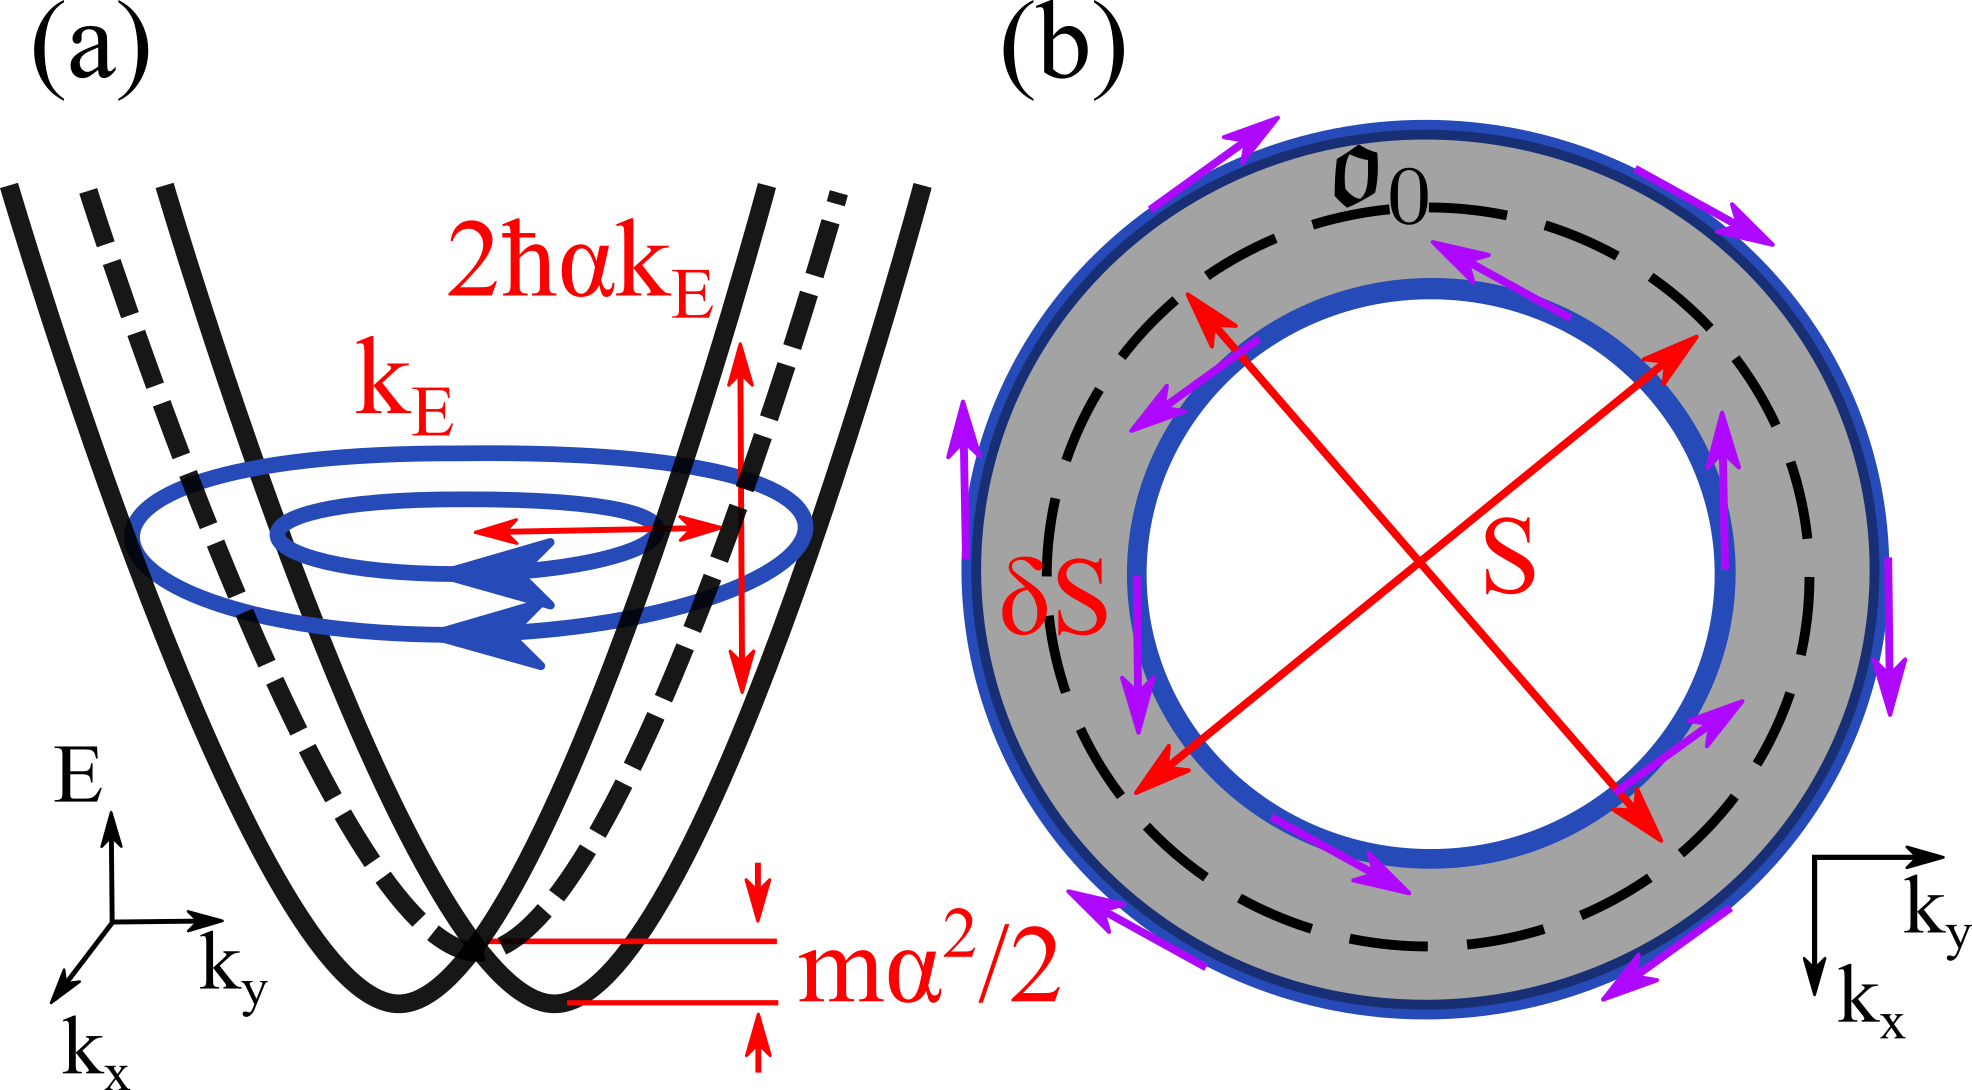
\includegraphics[width=0.9\columnwidth]{orbits.png}
\caption{(a) Solid (resp.\ dashed) lines respectively illustrate the band dispersion of an electron gas with (resp.\ without) Rashba spin-orbit coupling.  The oriented circles illustrate the spin-orit-split orbits for a magnetic field pointing to $-z$ direction. (b) The zeroth-order orbit $\frako_0$ is indicated by a dashed circle with area $S$; $\delta S$ is the differential area  between two spin-orbit-split orbits. The spin texture is indicated by purple arrows.\label{fig:orbits}}
\end{figure}


\subsection{Recovering the Onsager-Lifshitz-Roth quantization rules in two limits}\label{sec:recoveronsager}

It is useful to compare $\delta \var$ with $B\calm$ in the basis of energy-split bands (labelled $\pm$): in the two regimes where one dominates over the other, \qq{eq:rule}{berryconn} reduce to the known Onsager-Lifshitz-Roth rules for (i) two independent, nondegenerate orbits, and for (ii) degenerate orbits.  \\

%\footnote{Though the adiabatic limit does not exist for orbits that exactly intersect at type-II Dirac points, these orbits are nevertheless describable by our quantization rule, as exemplified in the case studies of \s{sec:inplanezeeman} and \s{sec:rotsymmbreakdown}.}}

\noi{i} If $|\var_+{-}\var_-|$ is everywhere (along $\frako_0$) much greater than $B|\calm_{+-}|$, then an electron would undergo adiabatic (band-conserving) dynamics[nenciu] along two independent, nondegenerate orbits. Such an adiabatic regime always exists as $B{\rightarrow} 0$ for quasidegenerate orbits that do not intersect, e.g, at a type-II Dirac point, which is the subject of the case studies in \s{sec:inplanezeeman} and \s{sec:rotsymmbreakdown}.
By  neglecting  $B\calm_{+-}$ in favor of intraband elements,  $\cala$ reduces to a diagonal matrix with  diagonal entries ($e^{i\lambda_{\pm}}$) given by:
\e{\lambda_{\sma{\pm}} = -\int_0^{T_c}\calh_{\sma{\pm\pm}}\f{dt}{\hbar}=\pm \f{1}{2}l^2\delta S - B\int_0^{T_c}\calm_{\sma{\pm\pm}}\f{dt}{\hbar}.  \label{phaseindependentorbit}} 
\q{eq:rule}, combined with \q{phaseindependentorbit}, may be identified as the Onsager-Lifshitz rule[onsager,lifshitz] for  two independent, nondegenerate orbits of areas $S{\pm}\delta S$, and with subleading phase corrections that were first identified by Roth[rothII].\footnote{We remark that \q{phaseindependentorbit} neglects the contribution by band $-$ to the orbital moment of band $+$: $\delta M_z=il^{-2}\epsilon_{\ab}(\delta \var_+-\delta \var_-)\mathfrak{X}^{\alpha}_{+-}\mathfrak{X}^{\beta}_{-+}$. $\mathfrak{X}^{\alpha}_{+-}$, being an off-diagonal matrix element of the position operator, is generically of order a lattice constant $a$. We then estimate $\int_0^{T_c} B\delta M_z dt/\hbar=O(a^2 \delta S )$, which is negligible compared to $l^2\delta S/2$. Note also that the single-band orbital moment simply vanishes in some symmetry classes of orbits.[100page] } The perturbative inclusion of $B\calm_{\sma{+-}}$ results in  a correction to $\lambda_{\pm}$ [cf.\ \q{phaseindependentorbit}] that is expressible as a power series in $B$, with a leading term proportional to $B$; this will be confirmed in a subsequent case study [cf.\ \q{lambdasmallB}] and applied to understand beatings in quantum-oscillatory phenomena in  \s{sec:qo}.    \\




%the hybridization parameter  $(l^2\delta S)^{-1}$ with the interband matrix elements of the generalized Zeeman interaction $\mathbb{Z}_{+-}{:}{=}B\int_0^{T_c}|\calm_{+-}|dt/\hbar$,  where \qq{eq:rule}{eq:H1} reduce to the known Onsager-Lifshitz-Roth rules for (i) two independent, nondegenerate orbits, and for (ii) degenerate orbits.  \\

%\noi{i} Let us consider the zero-hybridization limit ($l^2\delta S{\gg}1$) for two spin-orbit-split orbits that do not exactly intersect (e.g., at a type-II Dirac point\footnote{Though the adiabatic limit does not exist for orbits that exactly intersect at type-II Dirac points, these orbits are nevertheless describable by our quantization rule, as exemplified in the case studies of \s{sec:inplanezeeman} and \s{sec:rotsymmbreakdown}.}). 

\noi{ii} Let us consider the opposite regime where the Zeeman splitting due to $B\calm$ is much greater than $(\delta \var_+{-}\delta\var_-)$. \qq{eq:rule}{berryconn}, with $\calh{\approx}B\calm$, may then be identified with the quantization rule (formulated previously by us [topoferm,100page]) for degenerate orbits of any symmetry.\footnote{An equivalent but less general formulation was proposed earlier in [RothII] and [Mikitik,Sharlai] for centrosymmetric solids with time-reversal symmetry (at zero field). For comparison, it should be emphasized that \qq{eq:rule}{berryconn} applies to solids of any symmetry, including magnetically-ordered solids.}	   


%The competition between $B\calm$ and $\delta \epsilon$ decides 
%whether the spin-orbit-split energy bands are nontrivially hybridized by the magnetic field. More precisely, the competition is between $\delta \epsilon$ and the inter-band matrix elements of $B\calm$; the former (resp.\ latter) is always dominant for sufficiently weak (resp.\ large) field, as  we will illustrate in the case study of \s{sec:Rashba}. 


%This leading dependence originates from $\A$ being generated by $\delta \var T_c {\propto}1/B$ [cf.\ \qq{eq:prop}{eq:H1}]. 

%One motivation for the form of \q{eq:rule} is a separation of scales for different components of 

%Separating the semiclassical phase (acquired by a spinor wavepacket over one cyclotron period) into multiple components [as in \q{eq:rule}] may be motivated as a separation of scales. 
% in absolute magnitude, the rate of variation of $\partial l^2S$ (with respect to $E$ and $B$) is also much greater.


%Such non-analyticities might originate from saddle- or II-Dirac points of the zero-field Hamiltonian \textit{without} spin-orbit coupling. 





%is estimated to be $\sim\epsilon_c E/\Delta$, much larger than cyclotron energy $\epsilon_c$ due to $\Delta\ll E$. Therefore, the dependence of $\lambda_a$ on $E$ is also weak. 

The quantization rule, summarized by \qq{eq:rule}{berryconn}, is the technical accomplishment of this work; the remainder of this work is focused on unpacking its physical implications. We will first demonstrate the utility of our rule in case studies where the adiabatic approximation is invalid, and $\delta \epsilon$ competes with $B\calm$. There are two conceptually different ways in which the adiabatic approximation may fail: (i) if the spin-split orbits are  symmetric under continuous rotations (as they are for the Rashba 2DEG), then adiabaticity may be lost over the entire orbit [cf.\ \s{sec:Rashba}]. (ii) For asymmetric spin-split orbits, adiabaticity may be lost in the vicinity of a single isolated point, where orbits intersect at a type-II Dirac point [cf.\ \s{sec:inplanezeeman}]. 
In \s{sec:llquasideg}, we investigate how many real parameters are required to tune $\lambda_1{=}\lambda_2$ (mod $2\pi$), which would imply a (near) degeneracy of Landau levels.  

%In the absence of symmetry, three real parameters 
%certain symmetries  reduce the number of tuning parameters to one, as  will be investigated in \s{sec:llquasideg}. 



\section{Case study: Rashba 2DEG with arbitrarily-oriented fields}

%We begin with some preliminary remarks that apply to all case studies in this work. Our chosen studies are modeled (in zero field) by $\bk{\cdot}\bp$ Hamiltonians which are expanded (to quadratic order) about a high-symmetry wavevector ($\bk$). Our model Hamiltonians are written in a (pseudo-)spinor basis, i.e., they are two-dimensional at each $\bk$ [as exemplified by \q{eq:Rashba-Hamiltonian}]; this is the minimal dimension needed to model quasidegenerate orbits. 

%Any (pseudo-)spinor Hamiltonian can be  decomposed, at each $\bk$, into traceful ($\var(\bk)$) and traceless ($\delta \var$) components. We operationally identify the traceful component as the zeroth-order band Hamiltonian (with spin $\text{SU}(2)$ symmetry), and the traceless component as the spin-orbit term; the former produces spin-degenerate energy bands, and the latter splits the degeneracy. This identification has a microscopic justification: the Pauli spin-orbit coupling term  (that is derived from the non-relativistic limit of the Dirac equation) is  traceless in any spin-symmetric  (pseudo-)spinor basis.\footnote{The Pauli spin-orbit term is proportional to  $ \bs{\cdot} (\bE {\times} \bp)$. Viewing the spin-orbit coupling as a small parameter in degenerate perturbation theory, the lowest-order splitting of any spin-degenerate energy level is always symmetric about the zeroth-order energy. This follows because the zeroth-order, spin-symmetric wavefunctions (associated to a spin-degenerate level) are tensor products of spin and spatial wavefunctions: $\ket{\Psi_{\pm}}{:}{=}\ket{{\pm}\hat{n}}{\otimes} \ket{\psi}$ with $\hat{n}$ a unit vector and  $\bs{\cdot} \hat{n} \ket{{\pm}\hat{n}}{=}{\pm}\ket{\pm \hat{n}}$. Hence, $\braopket{\Psi_{\pm}}{\bs{\cdot} (\bE {\times} \bp)}{\Psi_{\pm}}{=}{\pm}\hat{n}\cdot\braopket{\psi}{\bE {\times} \bp}{\psi}$. } $H_0$ determines the zeroth-order orbit $\frako_0$ (and associated action $S$ and cyclotron energy $\var_c$). $H_{so}$ is simply identified with $\delta \var$, the spin-orbit term in the effective Hamiltonian $\calh$. One useful implication of this discussion is that $\delta \var$ is traceless.




\subsection{2DEG with Rashba and Dresselhaus spin-orbit interactions}\label{sec:Rashba}

%[ denoted by $\ket{u_{\pm,\bk}}=(1,\pm e^{i\theta_{\bk}})^t$ with $k e^{i\theta_{\bk}}=k_y+ik_x$ ]

%basis of spin-orbit-split energy  bands (defined at zero field), 

We will first apply our rule to the Landau levels of the Rashba model [cf.\ \q{eq:Rashba-Hamiltonian}], for which analytic expressions exist for verification; shortly after we will demonstrate the utility of our quantization rule for the 2DEG with both Rashba and Dresselhaus spin-orbit interactions, for which there exists no known analytic closed-form solution. 

For simplicity, we assume that the Pauli matrices in \q{eq:Rashba-Hamiltonian} correspond to spin: $s_i{=}\hbar \sigma_i/2$. Let us evaluate the effective Hamiltonian $\calh(\bk)$  along the cyclotron trajectory $\frako_0$ with radius $k$. In the  energy basis of the Rashba Hamiltonian $H_R$ [cf.\ \q{eq:Rashba-Hamiltonian}], 
\e{\calh(\bk)=-\alpha k\tau_z{+}\f{g_s}{2}\mu_{\sma{B}}B\tau_x {-} \f{eB\hbar}{2m} (\tau_x-I) \epsilon_{\alpha\beta} k_{\alpha}\nabla_{\beta}\theta,\label{rashbaeffham}}
where $\tau_i$ are a new set of Pauli matrices with $\tau_z{=}{+} 1$ and ${-}1$ corresponding to the outer and inner orbits, respectively. $e^{i\theta_{\bk}}{=}(ik_x{-}k_y)/k$ is the angle of the in-plane spin-splitting field $({-}\alpha k_y,\alpha k_x,0)$ of $H_R$, which winds once over $\frako_0$; the spin of our basis vectors likewise winds, in parallel (or anti-parallel) alignment with this field (see Fig. (\ref{fig:orbits})(b)). Terms proportional to the rate of spin rotation  ($\nabk \theta$) originate from the non-abelian Berry connection. The first term of  $\calh$ corresponds to the spin-orbit-induced splitting of the energy-degenerate bands;
the remaining terms may be interpreted as B-induced deformations of the bands.   It is well-known that the Zeeman term tends to polarize spin in the direction ($\vec{z}$) of $\bB$; remarkably, the non-abelian Berry term   also has a polarizing effect, but with opposite sign. These two effects completely cancel for free electrons ($m{=}m_0$, with $m_0$ being free electron mass.), but not generically in band systems. The orbital moment term $B M_z$, which generally couples the two-band subspace (of interest) to all other bands, is absent in any simplified two-band model.
%Observe that  that $\calh$ is actually time-independent, which originates from a  that is unbroken by the field (aligned with the rotational axis). Consequently, 

Due to the continuous rotational symmetry of $H_R$, $\nabk \theta$ has magnitude $1/k$ and lies tangential to $\frako_0$; consequently, $\calh$ is constant along $\frako_0$, and the propagator simplifies to $\cala{=}e^{{-}i\calh T_c/\hbar}$ without time-ordering, and the phase corrections to the quantization rule are simply the eigenvalues of $\calh$ multiplied by $T_c$:
\begin{equation}
\lambda_{\pm}=\pm\f1{2}\sqrt{({l^2\delta S})^2+\pi^2(g_sm/m_0-2)^2}+\pi. \label{eq:Rashba-lambda}
\end{equation}
This is a function of the differential area $\delta S$ [cf.\ \q{deltaSvsS}] and the effective mass $m$. The standalone $\pi$ term is the single-band Berry phase associated to the winding of $\theta_{\bk}$ by ${\pm}2\pi$. The two quantities under the square root originate from the spin-orbit energy splitting $\delta \var$ and the inter-band matrix elements of $B\calm$ (in the basis of zero-field bands). 

In the weak-hybridization regime: $l^2\delta S  \gg \pi|g_s m/m_0{-}2|$, we may expand \q{eq:Rashba-lambda} as a Laurent series in $B$:
\e{\lambda_{\pm}= \pm \f{l^2\delta S}{2} +\pi \pm \f{\pi^2}{4}\f{(g_sm/m_0-2)^2}{l^2\delta S} + O(B^2). \label{lambdasmallB}}
\q{eq:rule}, combined with the first two terms on the right-hand-side of \q{lambdasmallB}, may alternatively be derived from 
the standard Onsager-Lifshitz rules for two independent orbits, with a common $\pi$ Berry-phase correction for each orbit:\footnote{The intra-band Zeeman and orbital-moment couplings vanish due spacetime-inversion symmetry.[topoferm]} $l^2(S{\pm}\delta S)/2\pi {\in}\Z$. Higher-order terms in \q{lambdasmallB} reflect the field-induced hybridization of the spin-orbit-split orbits. 


In the strong hybridization regime: $l^2\delta S {\ll}\pi(g_sm/m_0{-}2)$, $\lambda_{\pm}{\approx}{\pm}\pi g_sm/2m_0$ mod $2\pi$, which corresponds to the Zeeman splitting of Landau levels by $g_{s}\mu_BB$, in the \textit{absence} of the spin-orbit interaction. 

%In the case of free electrons ($m{=}m_0$), we recover  an elementary result in quantum mechanics -- that all levels (except the lowest) are spin-degenerate due to the equality of cyclotron and Zeeman energies. 

%Eq. (\ref{eq:prop}) interpolates smoothly between the quantization rules for degenerate and independent orbits.

%For $\delta\epsilon=0$, Eq. (\ref{eq:prop}) is exactly the propagator for degenerate bands in Ref. [100p].

%If $\delta\epsilon$ dominates over all other terms in \q{eq:H1}, tunneling matrix elements between energy bands may be neglected. That is to say, the propagator is well-approximated by a diagonal matrix in the basis of energy bands; each diagonal element corresponds to the phase offset for an independent orbit.



%To better appreciate this, 
%$\A$ has the form:
%\begin{equation}
%\A=\overline{\exp}[i\oint_\frako_0\left(\begin{array}{cc}
%-\alpha l^{2}mk_F+\frac{1}{2} & -\frac{1}{2}+\frac{g'_s}{4}\\
%-\frac{1}{2}+\frac{g'_s}{4}& \alpha l^{2}mk_F+\frac{1}{2}
%\end{array}\right)d\theta],\label{eq:Rashba-prop}
%\end{equation}
%where $\theta$ is a polar angle parametrizing the cyclotron orbit, and $g_s'{:}{=}g_{s} m/m_0$ is an effective $g$ factor weighted by the ratio of the effective mass $m$ over the free-electron mass $m_0$. Off-diagonal elements of $\A$ induce inter-band tunneling, and are contributed by the Berry connection (the term $-1/2$) and the Zeeman coupling  ($g_s'/4$). That both terms are $k$-independent originate from the continuous rotational symmetry (in $z$ direction) of the Rashba Hamiltonian. 
%Diagonalizing Eq. (\ref{eq:Rashba-prop}), we obtain subleading order correction to quantization rule as

%The two quantities under the square root reflect a competition between intra- and inter-band matrix elements. The latter reflects a quantum interference between the Zeeman coupling and the non-abelian Berry connection, which is captured by our quasidegenerate quantization rule but absent in the standard Onsager-Lifshitz rules for independent orbits. To appreciate this, suppose we employ the standard rules[roth,100page] and properly account for the Zeeman coupling, the orbital moment, and the single-band Berry phase. The  Zeeman coupling  modifies the zero-field energy bands in two ways: it enlarges the spin-orbit-induced energy gap as $\Delta {\rightarrow} \Delta'{:}{=} \sqrt{(\Delta)^2{+}(g_s\mu_BB)^2}$, and it tilts the spin (along either orbit) out of the xy-plane. For $\Delta'{\gg}\var_c$, we may treat each Zeeman-deformed orbit as independent, and the corresponding Onsager-Lifshitz quantization rules are 
%\e{ l^2S\pm \lambda'_{\pm} = 2n(\pi+1/2), \;\text{with}\;   \lambda'_{\pm}:=\pm 2\pi \Delta'/\var_c{+}\pi.}
%The first component of $\lambda'$ is simply the modification of the WKB phase $l^2\delta S'$ due to both spin-orbit and Zeeman couplings; the second component is  the sum (${=}\pi$)[Fuchs,topoferm] encodes the single-band Berry phase and the orbital moment. A comparison of $\lambda_{\pm}$ with $\lambda'_{\pm}$ shows that the former has an extra $1/2$ under the square root [cf.\ \q{eq:Rashba-lambda}], which originates from the off-diagonal element of the non-abelian Berry connection. In other words, the standard Onsager-Lifshitz rules neglects the aforementioned quantum interference. This interference is completely destructive for free electrons ($m{=}m_0$), but not generically in band systems.

%\footnote{We have further assumed here that basis functions of $\mathcal{H}_R$ are eigenstates of spin operator $s_z$, which also need not be true in band systems. }

Our quantization rule [\q{eq:rule} with \q{eq:Rashba-lambda}] may be compared with the  exact Landau-level spectrum of the Peierls-substituted Hamiltonian $H_R(\bK)$. The exact levels are given implicitly by
\e{
&n_{\pm}=\frac{l^2S}{2\pi}+\frac{l^2\delta S}{16\pi}\f{\delta S}{S}\lin 
&\pm\f1{2}\sqrt{\bigg(\frac{l^2\delta S}{8\pi}\f{\delta S}{S}\bigg)^2+(l^2\delta S)^2+\pi^2(\f{g_sm}{m_0}-2)^2},\label{eq:Rashba-exact}}
with the functional forms of $\delta S(E)$ and $S(E)$ provided in \q{deltaSvsS};  $n_{+}{\ge} 1$ and $n_-{\ge} 0$ here are integer-valued labels for two distinct sets of levels.  In the quasidegenerate regime ($E{\gg}m\alpha^2$), terms involving $\delta S/S$ may be neglected and \q{eq:Rashba-exact} reduces to our quantization rule with $\lambda_{\pm}$ given by \q{eq:Rashba-lambda}.

Our quantization rule equally has utility where no closed-form analytic expression exists for the spectrum. Such is the case when we introduce a Dresselhaus spin-orbit coupling:
\begin{equation}
 H_{RD}(\bk)=\frac{{\hbar^2}k^2}{2m}+\alpha(k_{x}\sigma_{y}-k_{y}\sigma_{x})+\beta(k_{x}\sigma_{x}-k_{y}\sigma_{y}).\label{hamRD}
\end{equation}
In Fig.\ \ref{fig:RD}(b-d), a comparison is made between the Landau levels obtained from exact numerical diagonalization of $H_{RD}(\bK)$ (by standard techniques reviewed in App. \ref{sec:numerical}) and those obtained from the quantization rule. The difference in energies tends to increase with smaller field [compare the left and right panels of   \fig{fig:RD}(b)] and shows a strong positive correlation with $l^2\delta S(\alpha,\beta)^2/S$ [compare \fig{fig:RD}(c) with \fig{fig:RD}(d)] for various choices of the spin-orbit parameters $(\alpha,\beta)$. This correlation may be anticipated from \q{eq:Rashba-exact}, which analytically demonstrates how terms involving $l^2\delta S^2/S$ modifies the quantization rule in the case where $\beta{=}0$. For our chosen parameters,  the difference in energies does not exceed $2\%$ of $\var_c$ as $l^2\delta S^2/S$ varies over $[0,0.75]$.


%Perfect match between quantization rule and exact diagonalization can be observed in the left panel of \fig{fig:RD}(b) while slight deviations are seen for smaller magnetic field. In \fig{fig:RD}(c) we plot the errors in energies for various choices of the spin-orbit parameters $(\alpha,\beta)$, which does not exceed $2\%$ of $\var_c$ in the plot range. Larger errors are positively correlated with 
%$l^2\delta S^2/S$ (with $\delta S$ depending on both $\alpha$ and $\beta$), as shown in Fig. \ref{fig:RD}(d); see also \q{eq:Rashba-exact}, which analytically demonstrates how terms involving $l^2\delta S^2/S$ modifies the quantization rule in the case of $\beta=0$. 

In \s{sec:llquasideg} we will further motivate the study of $H_{RD}$ by investigating the prevalence of Landau-level degeneracies. 


%\red{Equation \ref{eq:Rashba-exact} indicates the error of quantization rule is mainly contributed by high order terms, such as terms proportional to $l^2 \delta S^2/S$. We plot in Fig. \ref{fig:RD}(c) $l^2 \delta S^2/S$, showing a strong positive correlation between $l^2 \delta S^2/S$ and error of quantization rules. 

%For a last numerical comparison, we plotted in Fig. \ref{fig:RD} (b) the Landau-level spectrum at fixed $\alpha$ and $\beta$ 

%For fixed $\alpha$ and $\beta$, Landau fan diagrams are presented in Fig. \ref{fig:RD} (b), showing perfect match at relatively large magnetic field and slight deviation in smaller magnetic field between quantization rule and exact Landau levels. 

%A typical constant energy contour of the band structure is shown in Fig. \ref{fig:errors} (a), where Dresselhaus SOC breaks continous rotational symmetry to two fold rotational symmetry. There are no known analytic closed-form solutions to the magnetic Hamiltonian $H_{RD}(\bK)$ obtained by Peierls subtitution of $H_{RD}(\bk)$; however $H_{RD}(\bK)$ can be numerically diagonalized by standard techniques that are reviewed in App. \ref{sec:numerical}. The difference between $\lambda$ calculated by numerical diagonalization and by Eq. \ref{eq:prop} are shown in Fig. \ref{fig:errors} (c), where good agreement can be observed. $\Delta/\epsilon_c$ of corresponding parameter range is presented in Fig. \ref{fig:errors}(b).

%$\lambda$ extracted from from Eq. (\ref{eq:Rashba-exact}) is consistent with what we have obtained in Eq. (\ref{eq:Rashba-lambda}). 

%It is instructive to consider what we would have obtained if we ignore the tunneling between the quasidegenerate orbits. Without tunneling, the quantization rule gives Eq. (\ref{eq:Rashba-exact}) with $(1/2-g_s'/4)^2$ missing under the square root. This difference is only relevant when $\epsilon_s$ is small enough such that this term dominates the square root, i.e., in the quasidegenerate range.

\begin{figure}
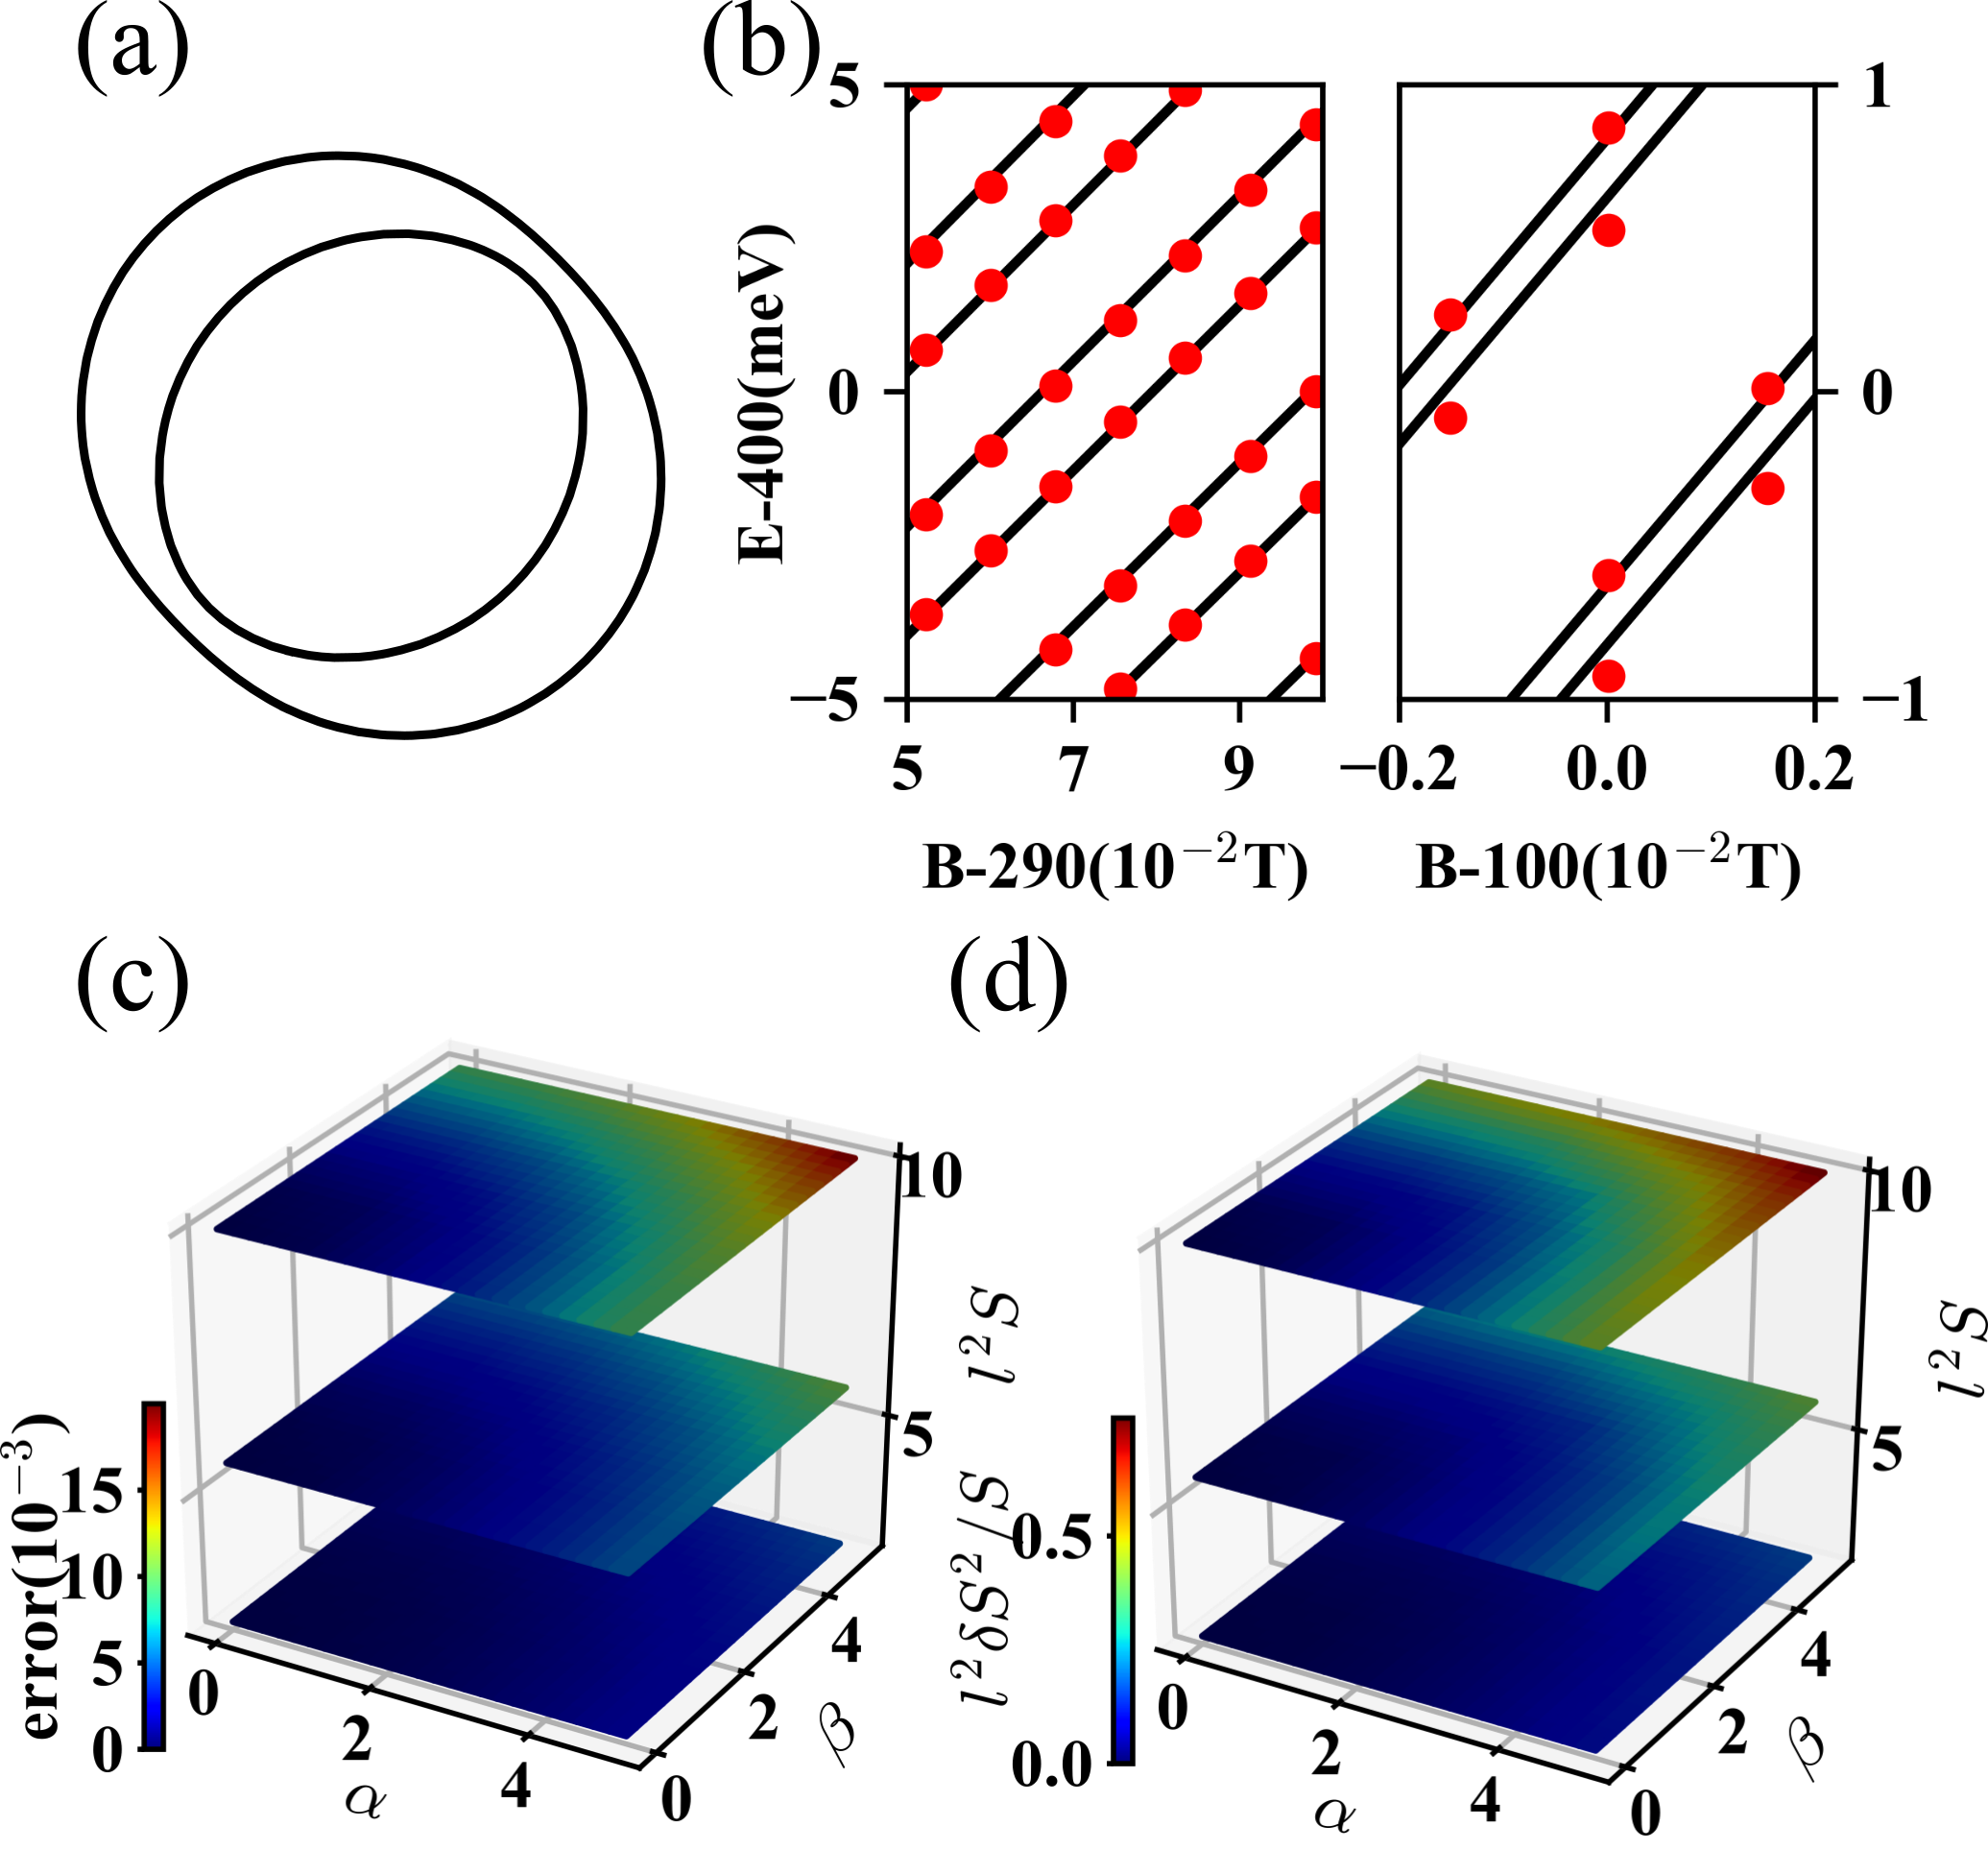
\includegraphics[width=1.0\columnwidth]{RD.png}
% alpha=0.05
% beta=0.02
% m=0.01
\caption{Rashba-Dresselhaus model. (a) Typical cyclotron orbits. (b) Comparison of Landau levels calculated by Eq. (\ref{eq:rule}) (black lines) and numerical diagonalization of the Peierls-Onsager Hamiltonian  $H_{RD}(\bK)$ (red dots). Parameters for (b): $\alpha=7.5$($10^{5}$cm/s$\cdot\hbar$), $m=0.076m_0$, $\beta=3~(6)$($10^{5}$cm/s$\cdot\hbar$) for left (right) panels. (c) For various spin-orbit parameters $(\alpha,\beta)$ of the Rashba-Dresselhaus model and various field strength (satisfying $l^2S(E)\gg 1$), we plot  $\text{error}:=|\epsilon_\text{rule}-\epsilon_\text{exact}|/\var_c$ for a single Landau level that lies closest to energy $E=0.4eV$, where $\epsilon_\text{rule}$ is determined by Eq. (\ref{eq:rule}) and $\epsilon_{\text{exact}}$ is obtained by numerical diagonalization of the Peierls-Onsager Hamiltonian  $H_{RD}(\bK)$. We also plot in (d) $l^2\delta S^2/S$, which has a strong positive relation with error in (c). Parameters for (c-d): $m=0.076m_0$. Units: $\alpha$($1.5\times 10^{5}$cm/s$\cdot\hbar$), $\beta$($1.5\times 10^{5}$cm/s$\cdot\hbar$), $l^2 S$($10^2$).\label{fig:RD}}
\end{figure}

\subsection{Rashba 2DEG with in-plane Zeeman field}\label{sec:inplanezeeman}


Our next case study involves orbits that (nearly) touch at a type-II Dirac point -- an asymmetric variant of the conventional Dirac point (as will be introduced below). Quantum tunneling localized to a type-II Dirac point  (in short, a II-Dirac point) is known to be mathematically equivalent to  Landau-Zener breakdown, with the electric force replaced by the Lorentz force.[Blount, Obrien, AALG] Here, we will demonstrate how  Landau-Zener dynamics emerge from our quantization rule [\qq{eq:rule}{eq:H1}], and explore (for the first time) how these dynamics are modified by the Zeeman effect. In particular, we will show that the perfect Klein tunneling predicted by O'Brien et al [OBrien] is never perfect with a proper account of the Zeeman effect. 

%\alpha(k_{x}\sigma_{y}-k_{y}\sigma_{x})+\zpar\sigma_{y}, 

We begin again with the Rashba model [cf.\ \q{eq:Rashba-Hamiltonian}] of a rotationally-symmetric Dirac cone. To convert this Dirac point to its asymmetric variant, 
let us introduce a Zeeman coupling to an in-plane magnetic field $B_\parallel$ (parallel to the $+y$ direction):
\e{ 
H_{RZ}=\f{{\hbar^2}k^{2}}{2m}+\delta \var; \;\;\;\delta \var=d_x\sigma_x+d_y\sigma_y,\lin
(d_x,d_y):=(-\alpha k_y,\alpha k_x+\zpar),\;\;\;\zpar:= g_s \mu_B B_{\parallel}/2.
\label{eq:RZ-Hamiltonian}}
While this field breaks both time-reversal ($T$) and two-fold rotational ($C_2$) symmetries, the composition $C_2T$ is preserved as $\sigma_x H^*_{RZ}(\bk)\sigma_x{=}H_{RZ}(\bk),$ which constrains spin to lie in-plane at each $\bk$. In this symmetry class, Dirac nodes are irremovable but movable   in two-dimensional $\bk$-space. The in-plane Zeeman field has the dual effect of  moving the Dirac node  to the position:
\begin{eqnarray}
\bar{k}_x & = & -\frac{\zpar}{\alpha},\;\bar{k}_y=0,\;\epsilon_{0}=\frac{{\hbar^2}\zpar^{2}}{2m\alpha^2},\label{whereisdiracpoint}
\end{eqnarray}
and tilting the Dirac cone. To observe this tilt, consider the linearized Hamiltonian in the vicinity of this node: 
\e{
H & =\alpha\left[\left(\sigma_y-\frac{{\hbar^2}\zpar}{m\alpha^2}\right)\delta k_{x}-\delta k_{y}\sigma_{x}\right]+\epsilon_{0}.}
When $|\hbar^2\zpar|>|m\alpha^2|$, the Dirac cone tilts over in the $x$ direction, leading to a Lifshitz transition  of the constant-energy band contours -- from circular to hyperbolic (in the linearized approximation), as illustrated in Fig. \ref{fig:RZ}(c). An over-tilted Dirac cone shall be referred to as type-II. Our case study of a II-Dirac point  connects  two electron-like  pockets [cf.\ \fig{fig:RZ}(a,c)], and  differs from previous case studies [OBrien, AALG] that connect an electron- and hole-like pocket.

\begin{figure}
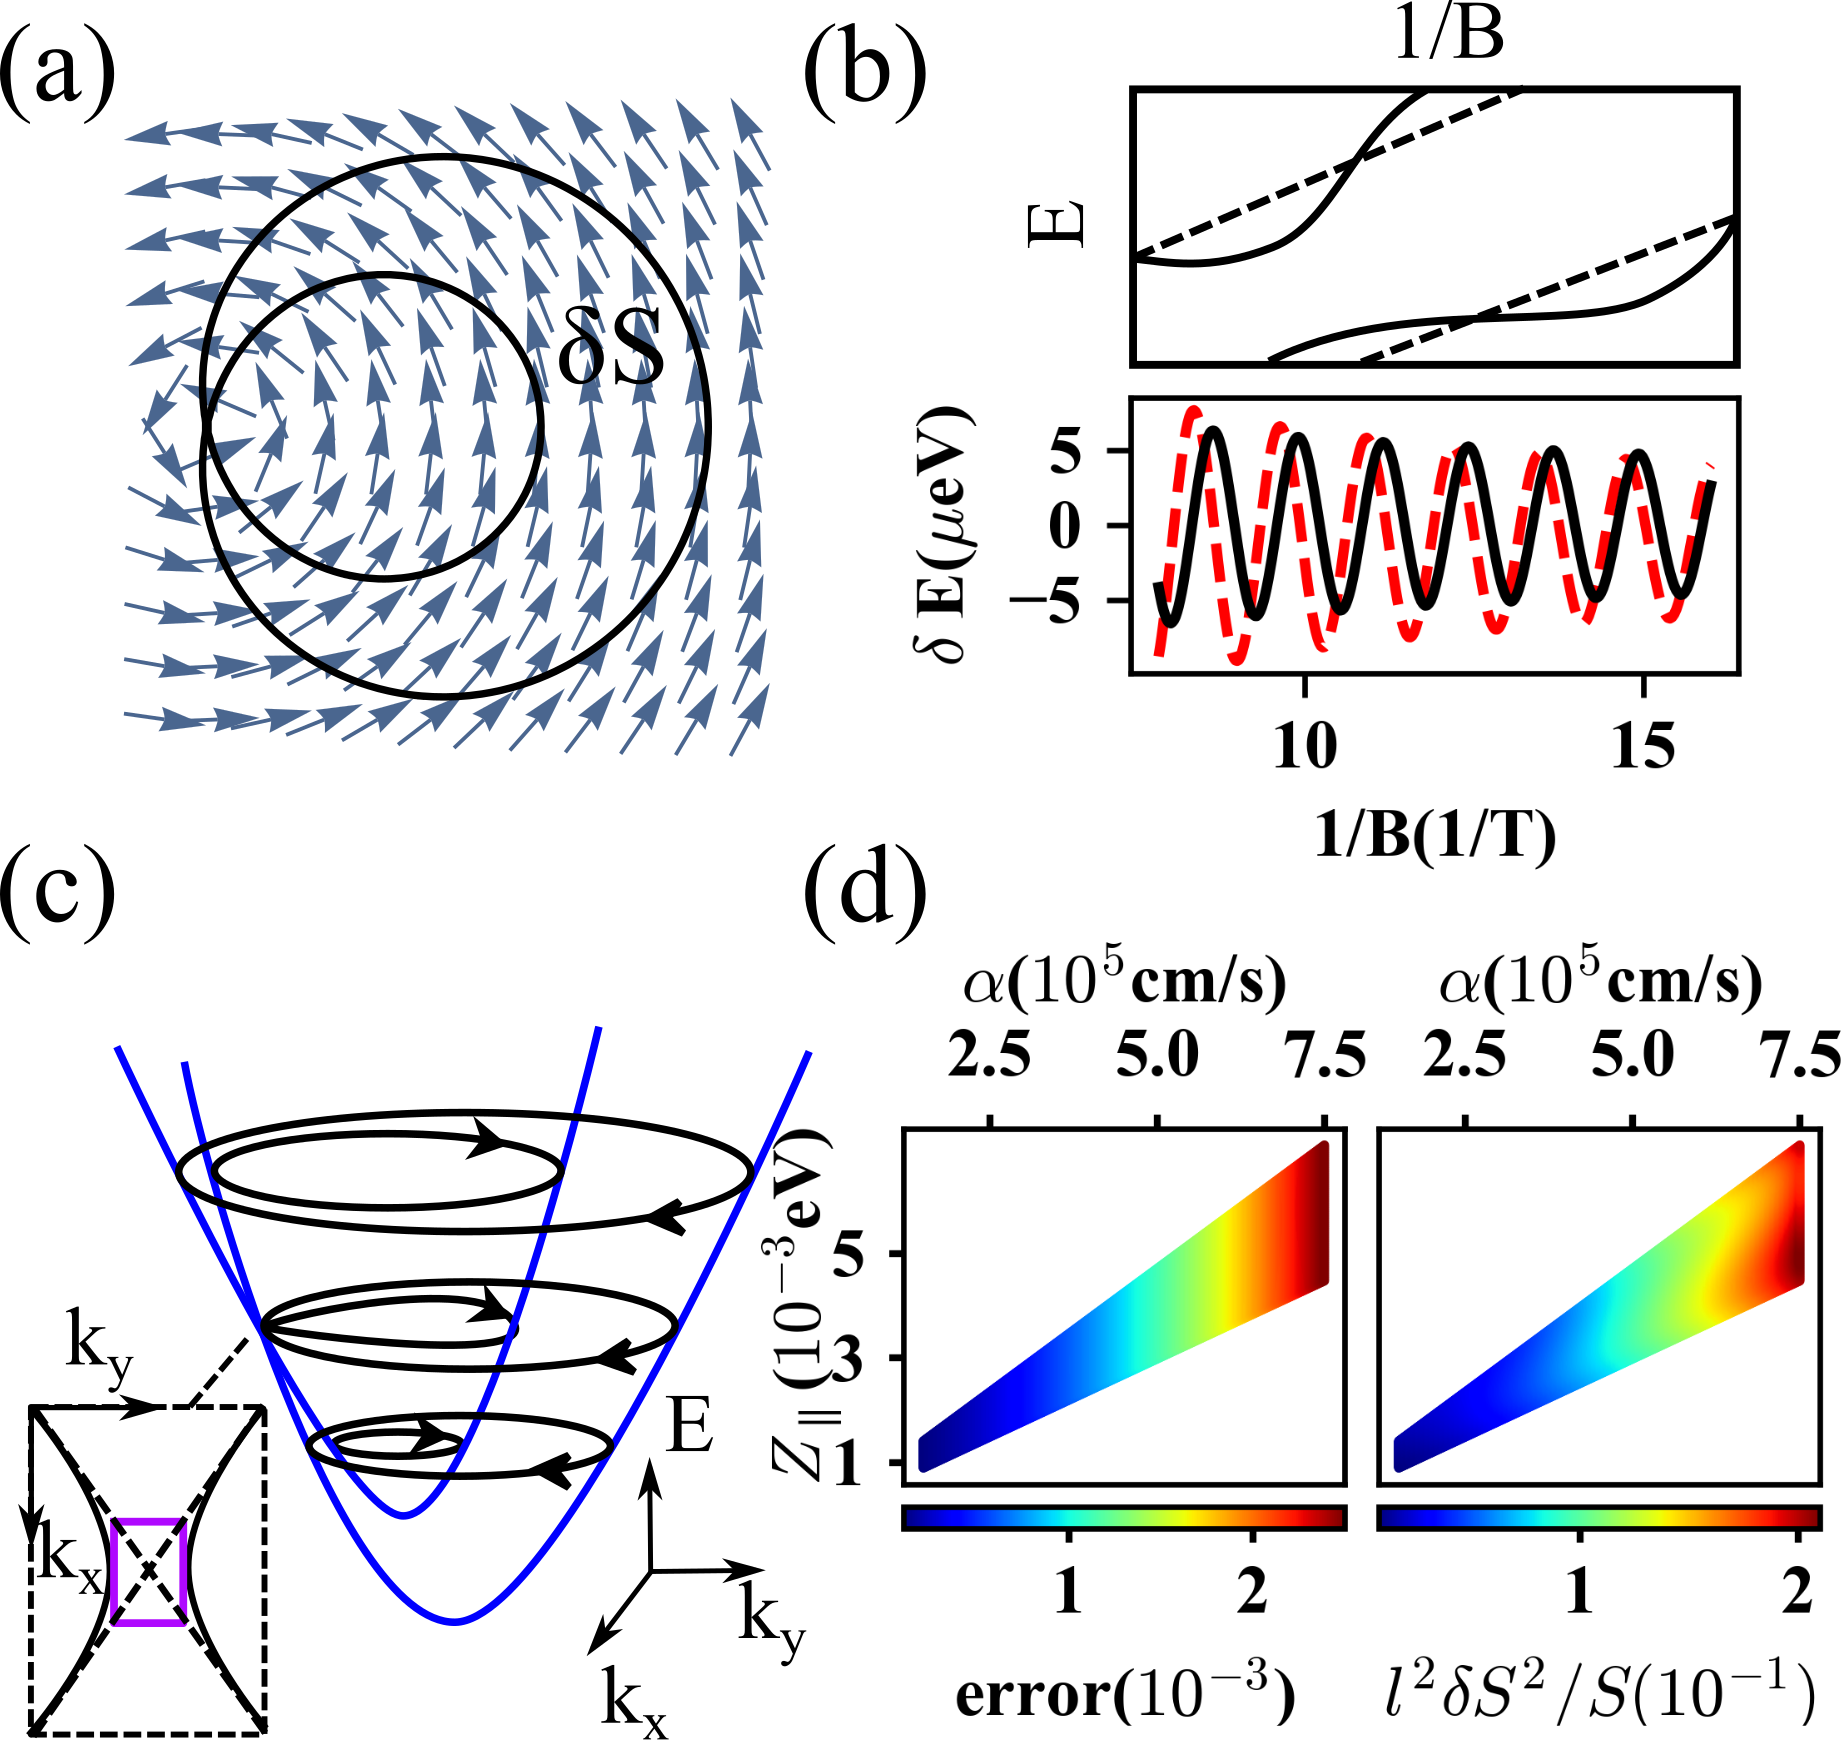
\includegraphics[width=1.0\columnwidth]{RZ.png}
\caption{(a) Trefoille-shaped cyclotron orbit for the Rashba-Zeeman model at the energy of the Dirac point. The orbit is drawn over the  spin-splitting field ($d_x,d_y$) of the degeneracy-lifting Hamiltonian $\delta\var$ [cf.\ \q{eq:RZ-Hamiltonian}]. The wavefunction along the inner (resp.\ outer) component of the trefoille orbit has its pseudospin aligned parallel (resp.\ anti-parallel) to the spin-splitting field. (b) Upper panel: a schematic illustration of Landau levels near the II-Dirac point of the Rashba model (with in-plane Zeeman field, and in the weak- hybridization limit). The solid line represents the Onsager-Lifshitz quantization of the trefoille orbit [cf.\ Eq.\ ({trefoillerule})], and the dashed line incorporates the first-order correction [cf.\ Eq.\ (\ref{RZfirstorderE})] due to tunneling. 
Lower panel: oscillation of $\delta E_n$ [cf. Eq. (\ref{RZfirstorderE})] for even integer $n$ with respect to magnetic field calculated by Eq. (\ref{RZfirstorderE}) (black dashed line) and numerical diagonalization (red solid line). $\delta E$ is extracted at the Landau level closest to 0.45eV and the II-Dirac point is located at 0.5eV. Parameters for lower panel of (b): $m{=}0.076m_0$, $\alpha{=} 1.5(10^{5}$cm/s$\cdot\hbar$), $Z_\parallel {=}$1meV. Out-of-plane Zeeman coupling is negligibly weak for the choice of $m$. (c) A sketch of cyclotron orbits of Rashba Hamiltonian with in-plane magnetic field. Inset: an enlarged view of near II-Dirac point. (d) For various configurations ($\alpha$, $Z_\parallel$) of $H_{RZ}$, we plot in left panel $\text{error}:=|\epsilon_\text{rule}-\epsilon_\text{exact}|/\var_c$ for a single Landau level that is closest to $\epsilon_0$ in Eq. (\ref{whereisdiracpoint}), where $\epsilon_\text{rule}$ is determined by Eq. (\ref{eq:rule}) and $\epsilon_{\text{exact}}$ is obtained by numerical diagonalization of the Peierls-Onsager Hamiltonian $H_{RZ}(\bK)$. Corresponding $l^2 \delta S^2/S$ are plotted in right panel. We only plotted in region where $0.4{<}\epsilon_0{<}1.0$(eV).\cite{RZfignote}, Units: $\alpha$($1.5\times 10^{5}$cm/s$\cdot\hbar$). Parameters for (d): $m=0.076m_0$, $l=100$\AA. \label{fig:RZ}}.
\end{figure}

In addition to the in-plane field, let us also apply an out-of-plane field $B_{\perp}$, with associated magnetic length $\lper{=}\sqrt{\hbar/eB_{\perp}}$, cyclotron energy $\var^{\sma{\perp}}_c{:}{=}\hbar^2/m\lper^2{:}{=}\hbar \omega_c^{\sma{\perp}}{:}{=}h/T_c^{\sma{\perp}}$ and Zeeman coupling to the spin magnetic moment:  $\zper{:}{=}{g_s}\mu_B B_{\perp}/2$. We shall assume  $1/\lper^2S{\ll}1$, where $S$ is the area of the zeroth-order orbit (with effective mass $m$ and radius $k_E{=}\sqrt{2mE}/\hbar$). For energies much greater than $m\alpha^2$ and $\zpar$, the quasidegeneracy condition ($\delta S/S{\ll}1$) is met, where $\delta S$ is the differential area induced by both spin-orbit and in-plane Zeeman couplings [see \fig{fig:RZ}(a)].  The smallness of $1/\lper^2S$ and $\delta S/S$ (with finite ratio $\lper^2\delta S$) justifies our application of the quantization rule [\qq{eq:rule}{eq:H1}],  with the effective Hamiltonian: 
\begin{equation}
\calh(t)=\alpha(k_{x}\sigma_{y}-k_{y}\sigma_{x})+Z_\parallel\sigma_{y}-Z_\perp\sigma_{z}.\label{calHRZ}
\end{equation}
$t$ here is a time variable which parametrizes the zeroth-order orbit:
$\bk(t){=}({-}k_E \cos \omega_c^{\sma{\perp}} t, k_E \sin \omega_c^{\sma{\perp}} t )$. In the momentum-independent spin basis of \q{calHRZ}, the non-Abelian Berry connection vanishes, hence the generalized Zeeman interaction $B_{\sma{\perp}}\calm$ simply reduces to the Zeeman interaction with the spin  moment: $Z_\perp\sigma_{z}$.

As alluded to in \s{sec:qtznrules}, the adiabatic limit of two independent orbits does not exist if the two spin-orbit-split orbits exactly intersect at a II-Dirac point. To investigate this failure of adiabaticity, let us study the Landau levels at energies close to the II-Dirac point ($\epsilon_0$). We focus first on the regime where, on average (over $\frako_0$), the energy splitting $|\delta \var_+{-}\delta \var_-|$ [cf.\ \q{eq:RZ-Hamiltonian}] is much greater than $B_\perp|\calm_{\sma{+-}}|$. Equivalently, we are in the regime where $\alpha k_{\sma{E}}{\gg}\var_c^\perp$.\footnote{The orbit-averaged energy splitting is of order $\alpha k_{\sma{E}}$ for energies near the Dirac point. $B_\perp|\calm_{\sma{+-}}|$ is simply the Berry contribution to the Zeeman interaction, and has the form of the right-most term in \q{rashbaeffham}; this term is of order $\var_c$.} This implies that the split orbits do not appreciably hybridize -- except in the vicinity of the II-Dirac point where orbits (nearly) touch.  Near this touching point (where $t{=}0$), the dynamics of a spinor electron is described by linearizing $\H$ [cf.\ \q{calHRZ}] with respect to $t$:
\e{
\calh = -\alpha k_{E}\omega^{\sma{\perp}}_c t\,\sigma_x+(Z_\parallel-\alpha k_{E})\sigma_y-Z_\perp\sigma_z,\label{effhamIIDirac}
}
The eigenbasis of $\sigma_x$ corresponds to two diabatic levels with characteristic slope $v_d{:}{=}\alpha k_E\omega^{\sma{\perp}}_c$; near $t{=}0$, the diabatic levels anticross  due to the hybridization terms proportional to $\sigma_{y,z}$. Generally, the probability of tunneling across the hybridization-induced barrier is  $\rho^2{=}\exp(-2\pi\barmu)$, with $\barmu{=}{E_g}^2/{2v_d \hbar}$ and $E_g$ the energy gap at the center of the anticrossing;[Landau and lifshitz, Wittig] in this context,
\e{\barmu=\frac{Z_\perp^2+(Z_\parallel-\alpha k_{E})^2}{2\alpha k_{E}\var^{\sma{\perp}}_c}, \label{mu1}}
with $2\alpha k_E$ the spin-orbit splitting at energy $E$ [cf.\ \fig{fig:orbits}(a)]. In the absence of the out-of-plane Zeeman coupling ($Z_\perp{=}0$), $\bar{\mu}$ would vanish at the energy of the II-Dirac point -- leading to unit-probability Klein tunneling, as was first proposed by [Obrien] in a different model of the II-Dirac point. However, with a proper account of $Z_\perp$, we find instead that $\bar{\mu}$ has a nonvanishing minimum: $\bar{\mu}_{\sma{\text{min}}}{:}{=} ( m/m_0)(Z_\perp/4\alpha k_{E})$, which is a product of the dimensionless effective mass and the ratio of the out-of-plane Zeeman splitting over the spin-orbit splitting. This minimum is practically negligible for  semiconductor heterostructures with $m{\ll}m_0$, but may be relevant in heavy-fermion systems. 

To determine the Landau levels, one needs not just the probability for tunneling but also the phase of the probability amplitude. The full information is encoded in a scattering matrix [AALG]
\e{\mathbb{S}=\matrixtwo{\tau e^{i\barphi}}{-\rho}{\rho}{\tau e^{-i\barphi}},\;\rho=e^{-\pi\barmu},\;\tau=\sqrt{1-\rho^{2}}\label{scattmat}}
which is a connection formula that matches the two-component semiclassical (WKB) wavefunction across the Dirac point. This formula  has been expressed in the basis of Zeeman-modified energy bands [i.e., eigenvectors of Eq.\ (\ref{calHRZ})]; diagonal (resp.\ off-diagonal) elements of $\mathbb{S}$ are amplitudes for intraband transmission (resp.\ interband tunneling). The phase of the intraband amplitude is $\barphi{:}{=}\barmu{-}\barmu\ln\barmu{+}\text{arg}[\Gamma(i\barmu)]{+}\pi/4$ with $\Gamma$ the gamma function.

Away from the II-Dirac point, an electron undergoes adiabatic (band-conserving) dynamics. The time-ordered, coherent process of Landau-Zener tunneling/transmission and adiabatic dynamics is described by the propagator:
\e{{\A}= \matrixtwo{\tau e^{i\bar{\varphi}}}{-\rho}{\rho}{\tau e^{-i\bar{\varphi}}} \diagmatrix{e^{i\tilde{\lambda}_-}}{e^{i\tilde{\lambda}_+}}. \label{propinplanezeeman}}
The adiabatic phase $\tilde{\lambda}_{\pm}$ is the sum of a dynamical phase ${\pm} l^2 \delta S/2$ and  the single-band Berry phase $\phi^B_\pm$, for the outer ($+$) and inner ($-$) orbit respectively. At energies far above the Dirac point ($|E{-}\epsilon_0|{\gg}|Z_{\perp}|$) where the Zeeman interaction is negligible, both orbits encircle the Dirac point and hence $\phi_{\pm}^B{\approx}{\pm}\pi$; far below the Dirac point, neither orbit encircles the Dirac point, leading to $\phi_{\pm}^B{\approx}0$. At intermediate energies, $\phi_{+}^B$ (resp.\ $\phi_{-}^B$) is a continuous and decreasing (resp.\ increasing) function of energy, as supported by the Bloch-sphere argument in Fig. \ref{fig:blochsphere}.


%consist of two parts: dynamical phase $\lper^2 \delta S$ with $\delta S'$ now accounting for both spin-split and Zeeman-split area corrections,

%{=}\int_{\sma{0}}^{\sma{T_c}}\calh_{jj}dt/\hbar$ is the cyclotron integral of the corresponding diagonal element of the effective Hamiltonian (in the energy-band basis). $\delta \Omega_{\pm}{=}{\pm}l^2\delta S/2$ plus a field-independent geometric phase (equal to the angle swept by the in-plane spin-orbit field $(\bk^2/2m_2{-}\mu,wk_x,0)$ along the spin-split trajectory; cf.\ discussion in \s{sec:Rashba}).  

\begin{figure}
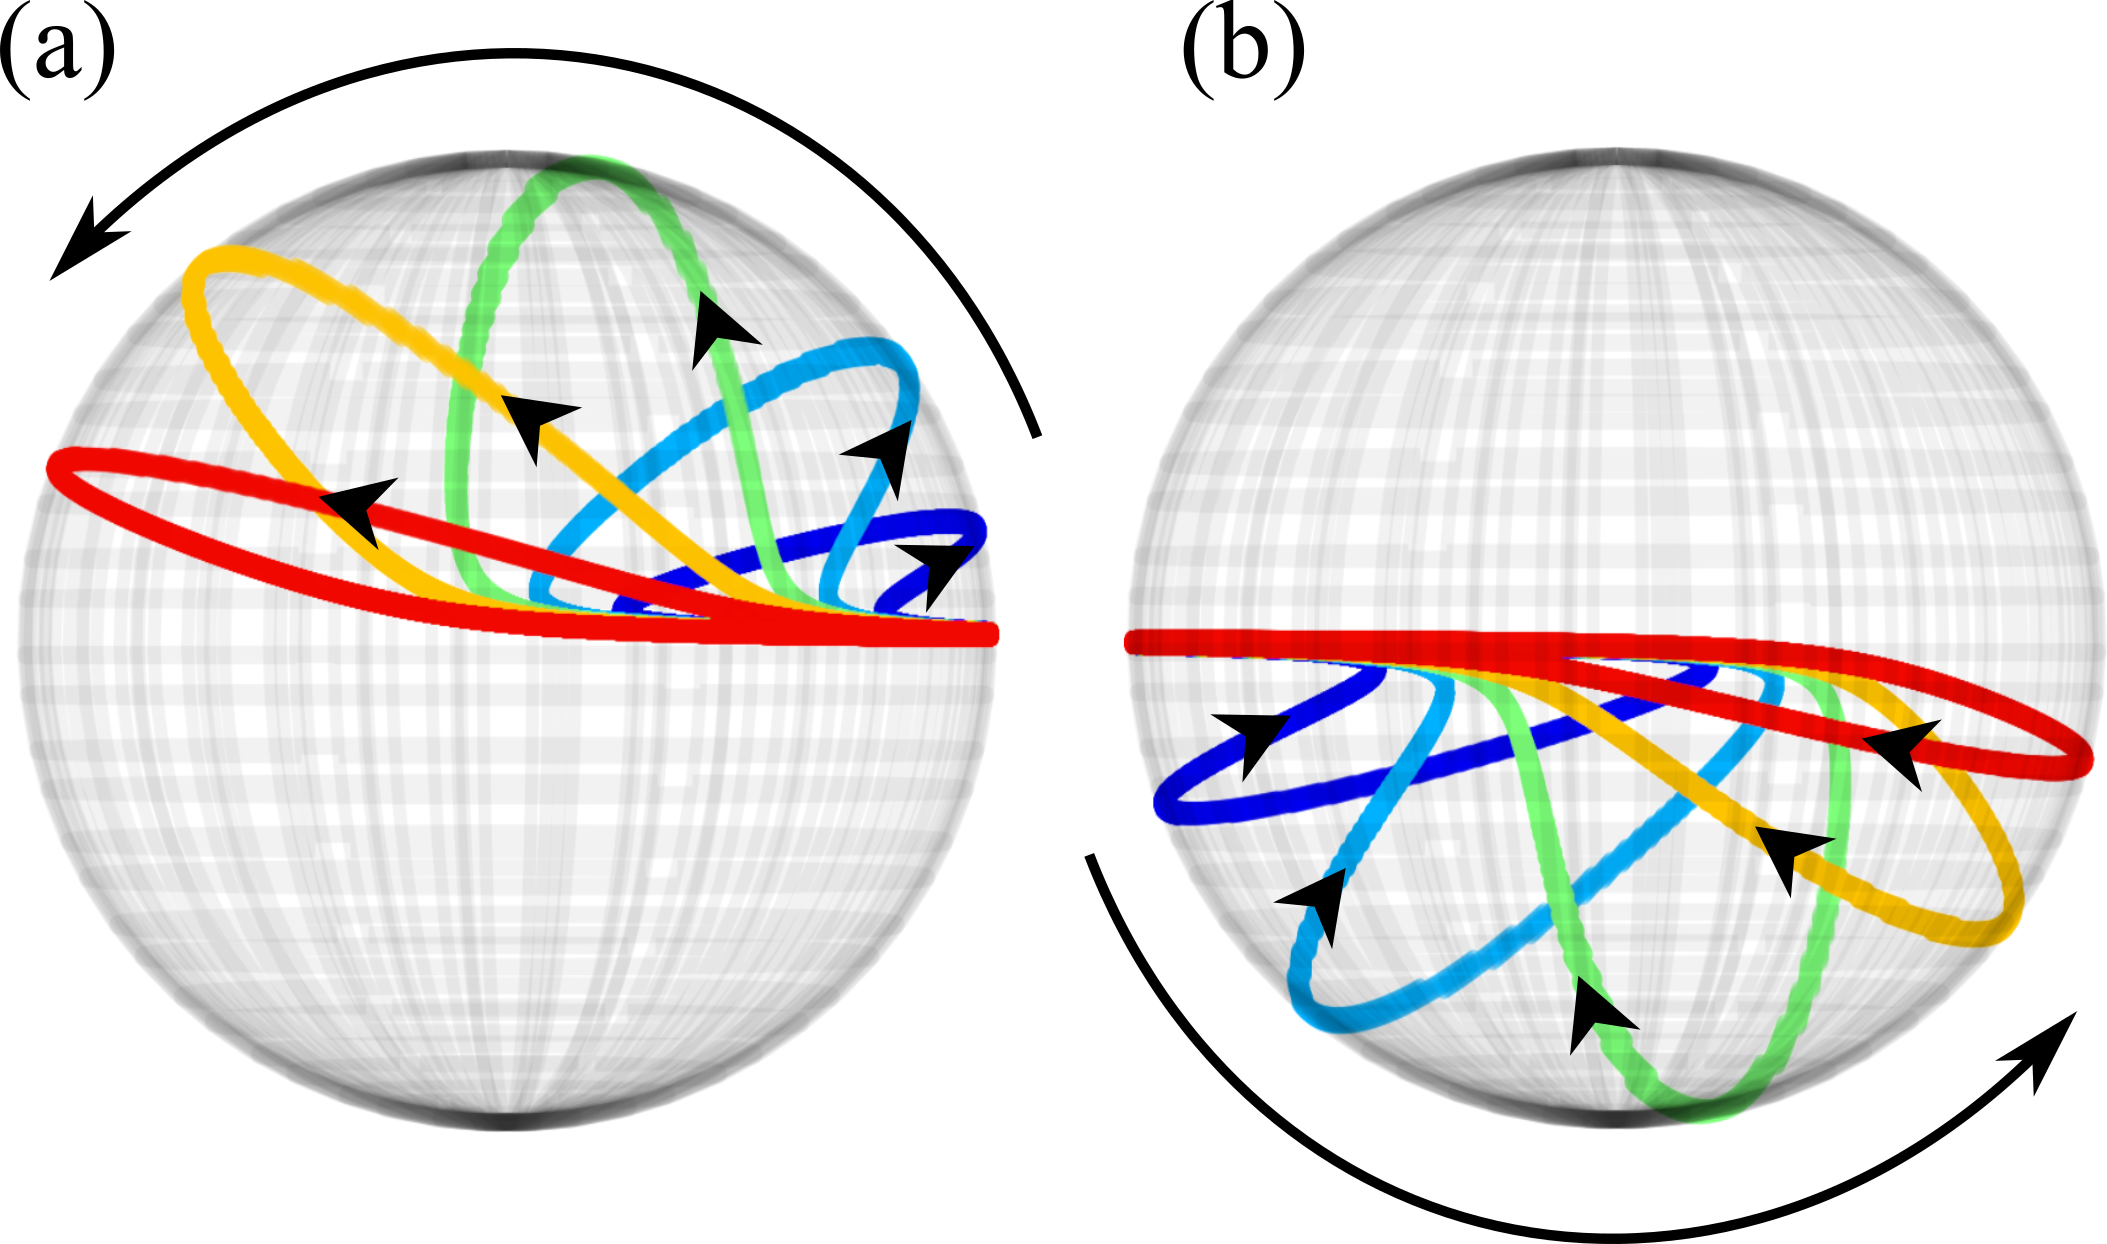
\includegraphics[width=1.0\columnwidth]{blochsphere.png}
\caption{Solid-angle representation of  the single-band Berry phase $\phi_{\pm}^B$ for inner (subscript $-$, upper panel) and outer ($+$, lower panel) orbit, at various energies close to the Dirac point $\epsilon_0$ [cf.\ Eq. (\ref{whereisdiracpoint})]. The decomposition of the effective Hamiltonian [cf.\ Eq. (\ref{calHRZ})] into  Pauli matrices ($\calh{=}\sum_j\calh_j\sigma_j$) defines a three-vector $\boldsymbol{\calh}{=}({-}\alpha k_y$,$Z_\parallel{+}\alpha k_x,{-}Z_\perp$). $\phi_{\pm}^B$ equals half the solid angle subtended by   ${\mp} \boldsymbol{\calh}(\bk)$ [solid blue line] as $\bk$ is varied along the outer/inner orbit;[Berry] the orientation of the solid angle is indicated by blue dotted lines. The out-of-plane Zeeman interaction lifts $\boldsymbol{\calh}$ out of the x-y plane, but this occurs at most over a fraction ${\sim}(\bar{\mu}_{\sma{\text{min}}}m_0/m{\ll}1)$ of the cyclotron period. \label{fig:blochsphere}}
\end{figure}

Our quantization rule [\qq{eq:rule}{eq:H1}], with $\A$ having the form of \q{propinplanezeeman}, may be equivalently expressed as
\e{
\text{cos}\left[\frac{\Omega_{-}+\Omega_{+}}{2}\right]=\tau\,\text{cos}\left[\frac{\Omega_{-}-\Omega_{+}}{2}+\bar{\varphi}\right], \lin
\ins{with}\;\Omega_{\pm}=l^2 (S\pm \delta S/2)+\phi_{\pm}^B +\gamma_{\pm}, \label{coscos}
}
$\Omega_{\pm}$ are phases acquired by an electron in adiabatically traversing the orbits labelled $\pm$, respectively; the quantum Maslov correction $\gamma_{\pm}{=}\pi$ for circular orbits.  A quantization rule analogous to \q{coscos} was previously derived by us for a II-Dirac point that intermediates an electron- and hole-like orbit [AALG]. 

%Let us first investigate the minimal- and maximal-tunneling limits for \q{coscos}. At energies away from the Dirac point ($E{\neq}\epsilon_0$) and in the limit $B{\rightarrow}0$, Landau-Zener tunneling is negligible ($\tau{\rightarrow}1,\bar{\varphi}{\rightarrow}0$), and \q{coscos} simplifies to the Onsager-Lifshitz-Roth rules ($\Omega_{\pm}/2\pi{\in}\Z$) for  two independent orbits. 

In the limit $\bar{\mu}{\rightarrow} \infty$, Landau-Zener tunneling is negligible ($\tau{\rightarrow}1,\bar{\varphi}{\rightarrow}0$), and \q{coscos} simplifies to the Onsager-Lifshitz-Roth rules ($\Omega_{\pm}/2\pi{\in}\Z$) for  two independent orbits.

For any nonzero field, $0{<}\tau{<}1$ implies that the two incommensurate harmonics $(\Omega_+{\pm}\Omega_-)$ in \q{coscos} compete to produce a quasirandom Landau-level spectrum [kaganovslutskin]. That is to say, the spectrum is disordered on the scale of nearest-neighbor level spacings but has longer-ranged correlations. To appreciate this, let us analyze the Landau levels (near the Dirac point) perturbatively in the small parameter $\tau$. To zeroth order, \q{coscos} reduces to
\e{2l^2S(E_n^0)+\pi = 2\pi n \rightarrow \{E_n^0(B)\}_{n\in\Z}.\label{trefoillerule}}
To derive the above equation, we have utilized $\phi^B_-{+}\phi^B_+{=}0$, which is valid for any two-band model in the quasidegenerate regime\footnote{For two band models, Berry phases of the two bands sum up to 0 on arbitrary path}; in \fig{fig:blochsphere} this is reflected in the sum of solid angles (at fixed energy) equalling $4\pi$. \q{trefoillerule} may be interpreted as a quantization rule for a trefoille-shaped orbit with net area $2S{=}4\pi m E{/\hbar^2}$; the corresponding Landau levels (sketched by solid lines in the upper panel of Fig. \ref{fig:RZ}(b)) are periodic in $E{\rightarrow}E{+}\pi/l^2(\partial S/\partial E)$ and in $l^2{\rightarrow}l^2{+}\pi/S$. Both periods are approximately half that of either disconnected  orbit, in the assumed quasidegenerate regime $\delta S{\ll}S$. The $\pi$ correction in \q{trefoillerule} is the Berry phase associated to a $2\pi$ rotation of the wavefunction spin over a single trefoille orbit, as illustrated in Fig. \ref{fig:RZ}(a). The Maslov phase, which is generally equal to $\pi$ times the rotation number of an orbit, is trivially $2\pi$ for the trefoille orbit.

To recapitulate, $E_n^0(B)$ [cf.\ \q{trefoillerule}] exhibits a periodicity on short scales associated to the large area of the trefoille orbit. This short-scale periodicity is lost due to  finite-$\tau$ corrections, yet a longer-range correlation (associated to the smaller differential area $\delta S$ between spin-split orbits) persists, as shown by the first-order-in-$\tau$ correction:\footnote{The general form of this perturbative calculation can be found in Sec. IX-E of [100page].} 
\e{&\delta E_n(B) = \f{(-1)^n}{2\pi} \tau \var_c^\perp \cos\bigg(\f{l^2\delta S}{{2}}+\f{\phi_+^B-\phi_-^B}{2}-\bar{\varphi}\bigg) \lin
    &\approx \f{(-1)^{n+1}m\alpha^2(E-\epsilon_0)(\var_c^{\perp})^{1/2}}{2\sqrt{\pi}\hbar^2
    Z_{\parallel}^{3/2}}\cos\bigg(\f{l^2\delta S}{{2}}-\bar{\varphi}\bigg),\label{RZfirstorderE}}
with the right-hand side (of each line) evaluated at $E{=}E_n^0(B)$. The second line is an approximation for $Z_{\perp}{\rightarrow}0$, and has greater utility where $m{\ll}m_0$. $E_n^{(0)}+\delta E_n$ are sketched in the upper panel of Fig. \ref{fig:RZ}(b) as dashed lines. The validity of Eq. (\ref{RZfirstorderE}) is confirmed by a comparison between $\delta E_n$ in Eq. (\ref{RZfirstorderE}) and $\delta E_n$ extracted from numerical diagonalization in the lower panel of Fig. \ref{fig:RZ}(b).

If the quasidegenerate orbits are appreciably hybridized ($\alpha k_{\sma{E}}{\lesssim}\var_c$), our quantization rule \qq{eq:rule}{eq:H1} remains valid but the propagator $\cala$ no longer has the closed analytic form of \q{propinplanezeeman}. We may anyway diagonalize $\cala$ numerically, and compare the resultant semiclassical Landau levels with the exact diagonalization of $H_{RZ}(\boldsymbol{K})$; to our knowledge, there exists no analytic solution of $H_{RZ}(\boldsymbol{K})$ for generic values of $\alpha,\zpar$ and $B_{\perp}$. For fixed  $B_{\perp}$ and a range of $(\alpha,\zpar)$ wherein  $l^2\delta S^2/S$ varies over $[0,0.2]$, the difference between semiclassical and exact Landau levels never exceeds  0.3\% of the cyclotron energy $\var_c$; this difference shows a strong positive correlation with $l^2\delta S^2/S$ [compare the left and right panels of Fig.\ \ref{fig:RZ} (d)], just like in the Rashba-Dresselhaus model. 

\section{Tuning the spin-degeneracy of Landau Levels}\label{sec:llquasideg}

We have argued in \s{sec:qtznrules} that the subleading corrections ($\lambda_{1,2}$) to the quantization rule [cf.\ \q{eq:rule}] generically lift the spin-degeneracy of Landau levels -- the level splitting is approximately $\var_c\delta \lambda/2\pi$ with $\delta \lambda=|\lambda_1-\lambda_2|$. Conversely, Landau levels are approximately spin-degenerate if $\lambda_1{=}\lambda_2$ (mod $2\pi$) -- this degeneracy condition for the eigenvalues of $\A$ may require fine-tuning of the Peierls-Onsager Hamiltonian.  

In \s{sec:relatedegeneracies}, we will describe the precise relation between eigenvalue-degeneracies of  $\A$ and (near) degeneracies of Landau levels. We then ask how many tunable real parameters are needed to attain an eigenvalue-degeneracy of $\A$. Our answer is  $3$ in the absence of symmetry, as discussed in \s{sec:introducecodimension}; the answer may reduce to $0,1$ or $2$ depending on the symmetry class of the orbit, as will be explained in \s{sec:tenfold}. Before this general symmetry classification,  we will first develop physical intuition by studying two rotationally-symmetric models [cf.\ \s{sec:singleparameterrashba} and \ref{sec:rotsymmbreakdown}] where only one tunable parameter is needed -- this can be the $B$ field itself.

%Finally, the experimental implications of single- and double-parameter tuning of Landau-level degeneracies are discussed in \s{sec:qo}.

\subsection{Relating the eigenvalue-degeneracy of $\A$ to the quasidegeneracy of Landau levels}\label{sec:relatedegeneracies}

Suppose the propagator $\A$ were degenerate at $(\bar{E},\bar{B})$, i.e., $\lambda_1(\bar{E},\bar{B})=\lambda_2(\bar{E},\bar{B})$ mod $2\pi$. Generically, $(\bar{E},\bar{B})$ is not \emph{simultaneously} a solution of the quantization rule in \q{eq:rule}. That is to say, $\bar{E}$ is not generically the energy of a Landau level at field $\bar{B}$. To obtain a Landau level, we may tune either $E$ or $B$   away from $(\bar{E},\bar{B})$, and  utilize that  $\lambda_{\pm}$ are slowly-varying functions of $(E,B)$ compared to $l^2S(E)$:
\e{l^2\left|\p{S}{E}\right| \gg \left|\p{\lambda_a}{E}\right|,\, \left|S\right| \gg \left|\p{\lambda_a}{l^2}\right|;} 
these inequalities are guaranteed by the quasidegeneracy condition ($\delta S{\ll}S$) and the smoothness of $S(E)$, as shown in \app{sec:slowvariation}.  For fixed $\bar{B}$, we are therefore guaranteed to find a number (of order one) of paired Landau levels  in close proximity to $\bar{E}$, with each pair having an energetic splitting of order:
\e{\bigg|\f{E_{1}-E_2}{\var_c}\bigg|_{B=\bar{B}} = \order\left( \f{\partial \lambda_a/\partial E}{\bar{l}^2\partial  S/\partial E}  \right)\ll 1,\label{llquasideg}}
with $\bar{l}$ the magnetic length associated to $\bar{B}$. Alternatively, we may fix $\bar{E}$ and investigate how Landau levels disperse as a function of $B$; the analog of \q{llquasideg}  is the existence of paired Landau levels in close proximity to $\bar{l}^2$, with a splitting of order:
\e{\bigg|\f{l^2_{+}-l^2_-}{T_{{l^2}}}\bigg|_{E=\bar{E}} = O\left( \f{1}{S}\p{\lambda_a}{l^2} \right)\ll 1,\;\; T_{{l^2}}:=\f{2\pi}{S(\bar{E})}.\label{llquasidegB} }
$\partial \lambda_a/\partial l^2$ is estimated in \app{sec:slowvariation}, and
$T_{l^2}$ above is the period (in $l^2$) of quantum oscillations -- in the absence of spin-orbit coupling. To recapitulate, for every exact degeneracy of $\cala$, there must exist, in close proximity, a number of paired Landau levels which are exactly degenerate, or nearly degenerate in the sense of \qq{llquasideg}{llquasidegB}. Each such pair of Landau levels will be called \textit{quasidegenerate}.

\subsection{Codimension analysis without symmetry, and with band-conservation symmetry}\label{sec:introducecodimension}


In the absence of symmetry,  eigenvalue-degeneracies of the unitary propagator $\A$ [cf. \q{eq:prop}] are attainable by tuning three real parameters. Analogously, it is well known (as the non-crossing rule in quantum theory[von Neumann,wigner]) that eigenvalue-degeneracies of complex, finite-dimensional matrix Hamiltonians are also attainable by tuning three real parameters.
 To prove the non-crossing rule for two-by-two unitaries, we begin by decomposing any such matrix as $\A{=}e^{i\phi}{\cal \bar{A}}$, with  ${\cal \bar{A}}{\in}\text{SU}(2)$. Then the necessary and sufficient condition for an eigenvalue-degeneracy of $\A$ is that ${\cal \bar{A}}{=}{\pm}I$. In the canonical parametrization of $\text{SU}(2)$ over the three-sphere $S^3$: 
\e{{\cal \bar{A}}{=}\matrixtwo{r_1{+}ir_2}{r_3{+}ir_4}{{-}r_3{+}ir_4}{r_1{-}ir_2},\;\; \sum_{j=1}^4r_j^2{=}1,\;\; r_j\in \mathbb{R},  \label{s3}}
${\cal \bar{A}}{=}{\pm}I$ lie on distinct points of $S^3$, and are attainable by tuning three real parameters: $r_2{=}r_3{=}r_4{=}0$. The conclusion that three parameters need be tuned remains valid for any  non-singular parametrization of SU$(2)$.


%If special unitaries were uniformly distributed over $S^3$, then encountering a spectral degeneracy for a randomly-selected special unitary would be an exceedingly rare event -- three parameters need be tuned to find either pole on $S^3$,  i.e., the codimension of degeneracy manifold is three. If only one  or two  parameters (in $\{r_1,\ldots,r_4\}$)  can be tuned, then in general we should not expect a degeneracy. 
 
 
 To generalize the above discussion, let us parametrize ${\cal \bar{A}}$ by $d$ independent real numbers  $\{r_1,\ldots,r_{d}\}{:}{=}\br $;  ${\cal \bar{A}}(\br){=}{\pm}I$ defines a set of submanifolds in $\br$-space which we refer to as degeneracy manifolds; in the above example, these manifolds comprise two points on $S^3$. The codimension of the degeneracy manifold  is defined as $d$ minus the dimension of said manifold; alternatively stated, the codimension is the number of linearly-independent parameters needed to fine-tune a degeneracy. Here and henceforth, we adopt the shorthand that  \textit{parameters} will always refer to real parameters, and \textit{codimension} always refers to a codimension of a degeneracy manifold. 

%, which may be viewed as imposing a $U(1){\times}U(1)$ symmetry.\footnote{$\cala$ commutes with any diagonal unitary matrix, with diagonal entries equal to two arbitrary $U(1)$ phase factors.} T

It is well-known that symmetry may reduce the codimension of Hamiltonians, e.g., an antiunitary symmetry may restrict complex Hamiltonians to real Hamiltonians, thus reducing codimension from three to two.[wigner,von neumann] In our context, an analog would be the symmetry of band conservation in the adiabatic regime (cf.\ \s{sec:qtznrules}), which restricts $\cala$ to have diagonal form  ($r_3{=}r_4{=}0$) in the basis of energy bands [cf.\ \q{phaseindependentorbit}]. The phase of $r_1{\pm}ir_2$ equals ${\pm} l^2\delta S/2$ plus field-independent corrections. Since this  phase alone  can be  tuned to attain $\cala{=}{\pm}I$, the codimension is unity. As a function of $l^2$, we deduce that Landau-level quasi-crossings occur  with a periodicity of $2\pi/\delta S$. This periodicity  has a dual interpretation  in real space -- as a periodic increment of a single flux quantum for  the differential magnetic flux (between the two split orbits).


We may ask if these quasi-crossings (based on band-conservation symmetry) persist at stronger fields where adiabaticity breaks down. If no symmetry remains, then the codimension is three [cf.\ \q{s3}], hence Landau-level quasi-crossings should not generically be found by varying $B$ alone. One of our main results is that  rotational symmetry (with rotational axis parallel to the field) results in degeneracy manifolds with unit codimension. This will be demonstrated by two  case studies: the Rashba 2DEG in \s{sec:singleparameterrashba}, and a model with II-Dirac points in \ref{sec:rotsymmbreakdown}. 



%The indicators defined above classifies symmetry operations into ten and only ten classes, presented in Tab.\ \ref{table:codimension}.



%In contrast,  $T\mathfrak{r}_x$ results in manifolds with codimension two. The latter result, in addition to a comprehensive codimension analysis for all symmetry classes, is presented in \s{sec:tenfold}. 


%The first study describes a Rashba-Dresselhaus 2DEG where the adiabatic approximation breaks down at all points along the semiclassical orbit; in the second study, the adiabatic approximation breaks down only in the vicinity of type-II Dirac points. 

%owing to a spacetime-inversion symmetry that simultaneous inverts space and time: $(\br,t){\rightarrow}({-}\br,{-}t)$, the zero-field Bloch Hamiltonian is Kramers-degenerate at each wavevector. However, this same symmetry is broken in the presence of a magnetic field, and therefore does \textit{not} reduce codimension in the Landau-level problem. 


\subsection{Codimension reduction for the Rashba 2DEG}\label{sec:singleparameterrashba}


In this and the subsequent section (\s{sec:rotsymmbreakdown}), we will demonstrate how rotational symmetry reduces codimension in the Landau-level problem. Before delving into this, it is instructive to consider the conceptually-simplest analog in differential geometry: if we parametrize the 2D plane by Cartesian coordinates $(x,y){\in}\R^2$, it is apparent that two parameters must be tuned to arrive at the origin. If however the origin is the center of a rotation symmetry, we may instead utilize polar coordinates and tune a single parameter (the radial coordinate) to arrive at $x{=}y{=}0$. We see that rotational symmetry reduces the codimension of the origin from two to one. Here, and in the  Landau-level problem, we define codimension with respect to a \textit{symmetrically-chosen coordinates} (if symmetry exists); such symmetric coordinates need not be well-defined at isolated high-symmetry points, just as the polar coordinates are not well-defined at the rotational center.


\subsubsection{With continuous rotational symmetry}\label{sec:ctsrot}

To understand why rotational symmetry reduces codimension in the Landau-level problem, we return to the Rashba model [cf. \ \q{eq:Rashba-Hamiltonian}] without in-plane Zeeman field. This model has a continuous rotational symmetry (denoted $\mathfrak{c}_{\infty}$), which manifests as the constancy of $\calh(\bk){:}{=}\sum_{j=1}^3r_j\tau_j$ over the circular zeroth-order orbit [cf.\ \q{rashbaeffham}]; here, $\br{=}(r_1,r_2,r_3)$ is a real three-vector and $\{\tau_j\}$ a set of Pauli matrices. Consequently, the propagator [cf.\ \q{eq:prop}] simplifies to the exponential form:
\e{\A{=}-\exp(-2\pi i\sum_{j}r_j\tau_j),\label{expform}}
where
\e{\br{=}\bigg(\f{g_sm}{4m_0}{-}\f1{2},0,-\f{\alpha k_{\sma{E}}}{\var_c}\bigg).}
Any $\text{SU}(2)$ matrix can be expressed in the exponential form [cf.\ \q{expform}] for some (possibly non-unique) $\br$, with $r_2$ not necessarily zero. We will demonstrate codimension reduction for the general form of $\A$ (having any $\br$), with the Rashba model as a particular realization.

All eigenvalue degeneracies of $\A$ occur on spheres in $\br$-space with radii $|\br|{=}\sqrt{r_1^2{+}r_2^2{+}r_3^2}$ equal to an integer ($j$)  multiple of $1/2$;  ${j}$ is odd (resp. even) for  $\A{=}I$ (resp.\ $\A{=}{-}I$).  This condition $|\br|{=}j/2$ (for any nonzero $j$) may be attained by tuning a single parameter. In other words,
all nonzero-radius spheres are unit-codimensional surfaces (known as hypersurfaces), whose stability rely on $\mathfrak{c}_{\infty}$ symmetry. These hypersurfaces separate $\br$-space into infinitely-many, distinct connected components, i.e., the zeroth homotopy group $\pi_0$ comprises an infinite set. Each hypersurface may thus be viewed as a symmetry-protected, topological defect, which separates domains (in $\br$-space) where Landau levels are non-quasidegenerate. By varying $B$ alone (at fixed energy), one then transits between different domains; each penetration of a hypersurface is accompanied by a Landau-level quasi-crossing. For the exactly-soluble Rashba model ($r_2{=}0$), these $\mathfrak{c}_{\infty}$-protected quasi-crossings  are consistent with (and partially explain)  the abundance of \textit{exact} level crossings in the spectrum of $H_R(\bK)$ [cf.\ \q{eq:Rashba-exact}], which would otherwise seem mysterious in face of  the Wigner-von Neuman non-crossing rule[wigner neumann].


The zero-radius sphere (i.e., a point) has codimension three, as would be expected if symmetry were absent [cf.\ \s{sec:introducecodimension}].    This point degeneracy can be understood from an elementary result in quantum mechanics: taking $\alpha{=}r_2{=}0$ \textit{and} $m{=}m_0$, we recover the Zeeman-split Landau levels of a free electron gas without spin-orbit coupling; all levels (except the lowest) are spin-degenerate owing to the equality of the Zeeman and cyclotron energies.[LandauLifshitzstatphysI]

The above discussion is reminiscent of topological (semi)metals which host Dirac-Weyl points and/or line nodes (of Bloch-Hamiltonian degeneracies). Both Dirac points (in 2D $\bk$-space, e.g., graphene) and  line nodes (in 3D $\bk$-space) are attainable by tuning two wavenumbers; the stability of such codimension-two manifolds
 relies on crystallographic point-group symmetries. On the other hand,  Weyl points in 3D $\bk$-space have codimension three and do not require any  point-group symmetry for their stability. Just like Weyl points, the point degeneracy of $\A$ is associated with a nontrivial Chern number (defined as an integral of the Berry curvature\footnote{The curvature is defined with respect to a line bundle formed from the nondegenerate eigenvector of $\cala$.} over a Gaussian surface surrounding the point). 


\begin{figure}
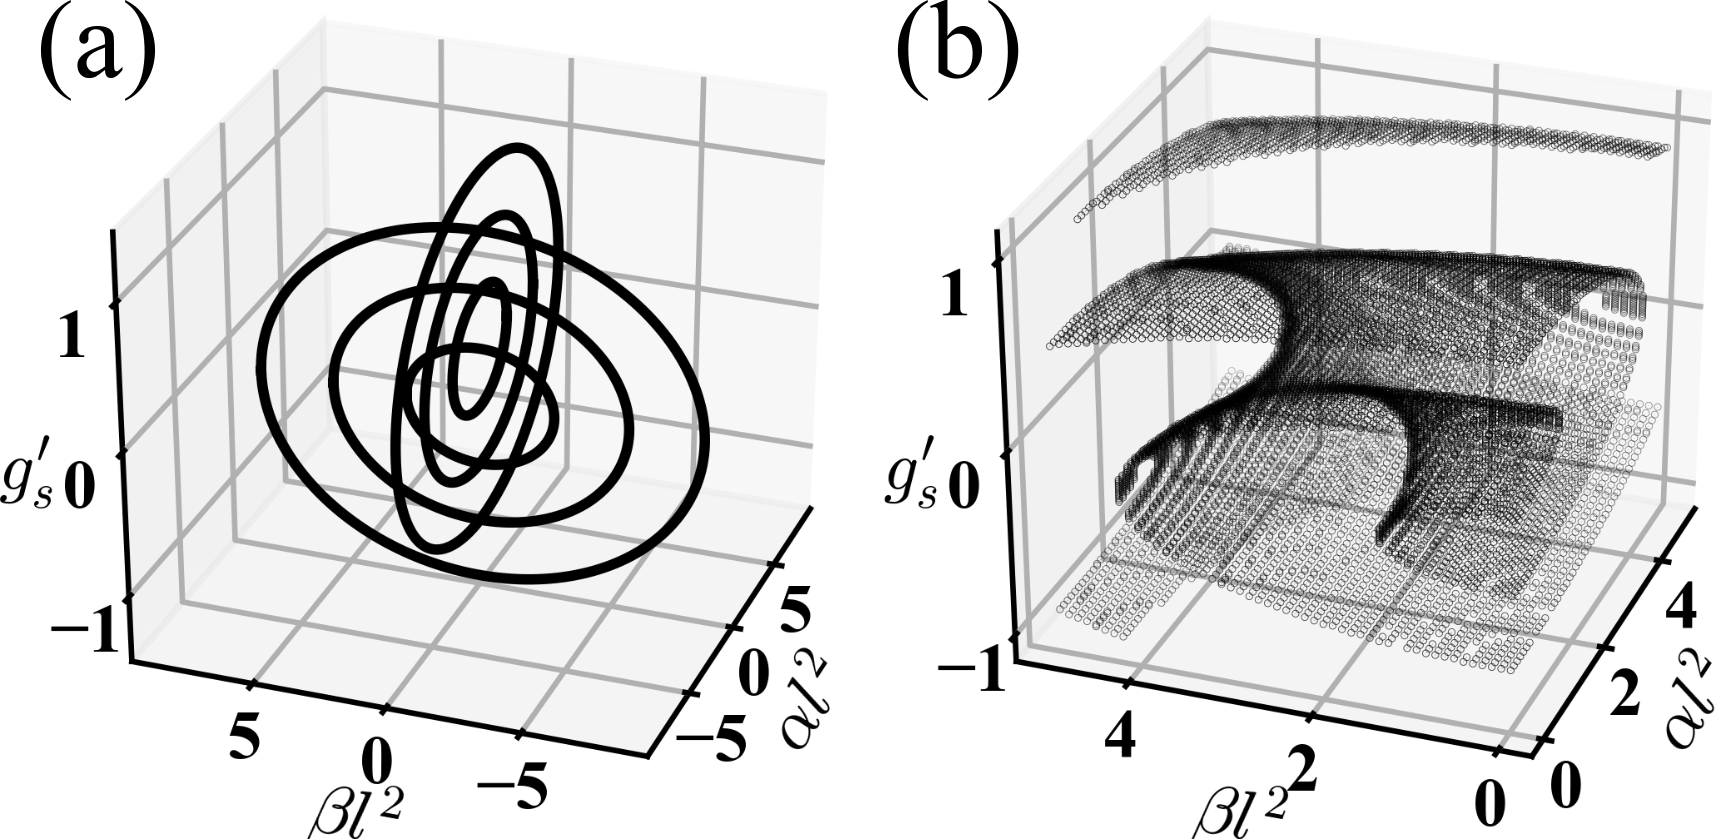
\includegraphics[width=1.0\columnwidth]{dgn.png}
\caption{Degeneracy manifolds of the Rashba-Dresselhaus model. (a) The degeneracy manifold of $\A{=}I$ is a path-connected hypersurface. Points in $\alpha=0$ or $\beta=0$ planes are colored in red. (b) illustrates the degeneracy manifold of $\A=-I$, which lie confined to  the $\alpha{=}0$ and $\beta{=}0$ planes (blue translucent planes). Each $\mathfrak{c}_{\infty}$-symmetric plane contains an infinite set of concentric, circular line degeneracies. Every circle (except for the smallest in either plane)  intersects two other circles in an orthogonal plane, such that the entire line node is path-connected. \label{fig:dgn}}
\end{figure}

\subsubsection{With discrete rotational symmetry}\label{sec:disrot}


The Rashba model suffers from an oversimplification -- continuous rotational symmetry is not a symmetry in any crystallographic space group. It is possible for $\mathfrak{c}_{\infty}$-symmetric $\bk{\cdot}\bp$ models to approximate Bloch Hamiltonians (defined over the Brillouin torus) with a discrete, order-$N$ rotational symmetry (denoted $\mathfrak{c}_N$). How robust are the above-mentioned Landau-level quasi-crossings  (over the $B$ axis) when $\mathfrak{c}_{\infty}$ symmetry is perturbatively reduced to $\mathfrak{c}_N$? For any  integer $N{\geq}2$, we find that $N{-}1$ of every $N$ quasi-crossings  are perturbatively stable. This general statement is proven in App. \ref{app:codimension}, and here we illustrate it for a specific model of $N{=}2$ -- we will reduce the $\mathfrak{c}_{\infty}$ symmetry of the Rashba model [cf.\ \q{hamRD}] to  $\mathfrak{c}_2$  by adding the Dresselhaus spin-orbit term (${\propto} \beta$).  

Since $\A$ depends on $\alpha,~\beta,~l,~E,~m$ only through $\alpha k_E /\var_c$, $\beta k_E /\var_c$ and $g_sm/m_0$, let us consider the three-dimensional parameter space $(\alpha k_{\sma{E}}/\var_c,\beta k_{\sma{E}}/\var_c,g_sm/m_0){\in} \mathbb{R}^3$.  $\A(\alpha k_{\sma{E}}/\var_c,\beta k_{\sma{E}}/\var_c,g_sm/m_0){=}{\pm} I$ determines a set of concentric circles in the $\beta{=}0$ plane, as per the $\mathfrak{c}_{\infty}$-symmetric case study in \s{sec:ctsrot}. Moving off this plane, we find that $\A{=}I$ is satisfied in a  neighborhood of $\beta{=}0$, i.e., $\A{=}I$ defines a hypersurface in $\mathbb{R}^3$ that is illustrated in \fig{fig:dgn}(a). On the other hand, $\A{=}{-}I$ is not satisfied in the neighborhood of $\beta{=}0$, hence the circles associated to $\A{=}{-}I$ remain isolated as line nodes, as illustrated in \fig{fig:dgn}(b). To recapitulate, we have found that one of every two Landau-level crossings (those labelled by odd $j$) destabilize due to the symmetry reduction.

\textbf{[Bonus content:consider the Berry phase of the eigenstate of A. Is it quantized for a symmetrically chosen loop in r space?]}
%If a line node (in the $\beta{=}0$ plane) were perturbatively stable to finite $\beta$, then it would be embedded in a two-dimensional degeneracy hypersurface of $\mathbb{R}^3$; if the planar line node were unstable, this embedding does not happen, i.e., the planar line node is simply a line node in $\mathbb{R}^3$. Our numerical study shows that half the planar line nodes (corresponding to $\A{=}I$) are stable, while the other half ($\A{=}{-}I$) destabilizes. In $\mathbb{R}^3$, we then have pairs of line nodes and hypersurfaces enclosed by increasingly larger pairs of line nodes and hypersurfaces, as illustrated in Fig. \ref{fig:dgn}. 

To demonstrate how the $\A{=}I$ hypersurface derives from $\mathfrak{c}_2$ symmetry, consider  the effective Hamiltonian $\calh$ 
\e{\calh=\alpha (k_{x}\sigma_{y}{-}k_{y}\sigma_{x})+\beta (k_{x}\sigma_{x}{-}k_{y}\sigma_{y})-\f{g_s}{2}\mu_{B}B\sigma_z,}
in a momentum-independent basis where the Pauli matrices correspond to spin operators. The two-fold rotational symmetry 
\e{\calh(\bk)=\sigma_z\calh(-\bk)\sigma_z, \;\: \bk(t)=-\bk\big(t+\f{T_c}{2}\big)\in \frako_0,}
implies that the propagator over the time interval $[T_c/2,0]$ is symmetry-related to that over $[T_c,T_c/2]$:
\e{\A=\A_{T_c\leftarrow T_c/2}\A_{T_c/2\leftarrow 0}=\sigma_z{\A}_{T_c/2\leftarrow 0}\sigma_z {\A}_{T_c/2\leftarrow 0}.\label{eq:sigmazconstraint}}
The tracelessness of $\calh$ (at each $\bk$) implies that  ${\A}_{\sma{T_c/2\leftarrow 0}}$  has unit determinant. 
Utilizing the canonical parametrization for this $\text{SU}(2)$ matrix [Eq. (\ref{s3}) with ${\cal \bar{A}}$ replaced by ${\A}_{\sma{T_c/2\leftarrow 0}}$], we derive 
\e{
{\A}={\cal \bar{A}}=\matrixtwo{1{-}2r_2(r_2{-}ir_1)}{2ir_2(r_3{+}ir_4)}{{-}2ir_2(r_3{-}ir_4)}{1{-}2r_2(r_2{+}ir_1)} \label{proprashba}
}
with $\sum_{j=1}^4r_j^2{=}1$. It follows that $r_2{=}0$ is a necessary and sufficient condition for $\bar{\A}{=}I$. The corresponding degeneracy manifold is a path-connected hypersurface, which separates $\br=(r_1,r_2,r_3,r_4)$-space into two distinct connected components. Generally, degenerate manifold of $\A$ of $\mathfrak{c}_N$ symmetric Hamiltonian separates $\br$-space (parametrizing $1/N$ of $\A$) into $N$ distinct connected components. \fig{fig:dgn}(a) illustrates the $\A=-I$ degenerate manifold in distinct coordinates: $(\alpha k_{\sma{E}}/\var_c,\beta k_{\sma{E}}/\var_c,g_sm/m_0)$. On the other hand, ${\cal \bar{A}}{=}{-}I$ occurs if and only if $\br{=}(0,\pm 1,0,0)$. These two points are mapped to a path-connected line node confined to the $\alpha{=}0$ and $\beta{=}0$ planes [cf.\ \fig{fig:dgn}(b)]; the difference in codimension originates from the  $\mathfrak{c}_{\infty}$ symmetry within these two planes [cf.\ \s{sec:ctsrot}], which was not accounted for in the $\mathfrak{c}_2$-symmetric analysis of \q{proprashba}. 

%If $C_2$ were the only symmetry, then three parameters would be needed to tune ${\cal \bar{A}}{=}{-}I$. Generally, additional symmetry further constrains $\bR$, which may effectively reduce the number of tuning parameters.  This explains why the ${\cal \bar{A}}{=}{-}I$ manifolds, as plotted in \fig{fig:dgn}(a)], are line nodes instead of point nodes: these line nodes lie in either the $\alpha{=}0$ or the $\beta{=}0$ plane, both of which are $\mathfrak{c}_{\infty}$-symmetric.\footnote{To complete the explanation, \textbf{speculative:} the space of $C_{\infty}$-symmetric unitaries lie on lines in $\bR$-space that intersect $\bR{=}(0,1,0,0)$ [the point node]. A singular coordinate transformation to $\br$-space maps these $C_{inf}$-symmetric lines to $\mathfrak{c}_{inf}$-symmetric planes, and the point node to a line node.}


\subsection{Codimension reduction for 2DEG with distinct, symmetry-related II-Dirac points}\label{sec:rotsymmbreakdown}

\begin{figure}
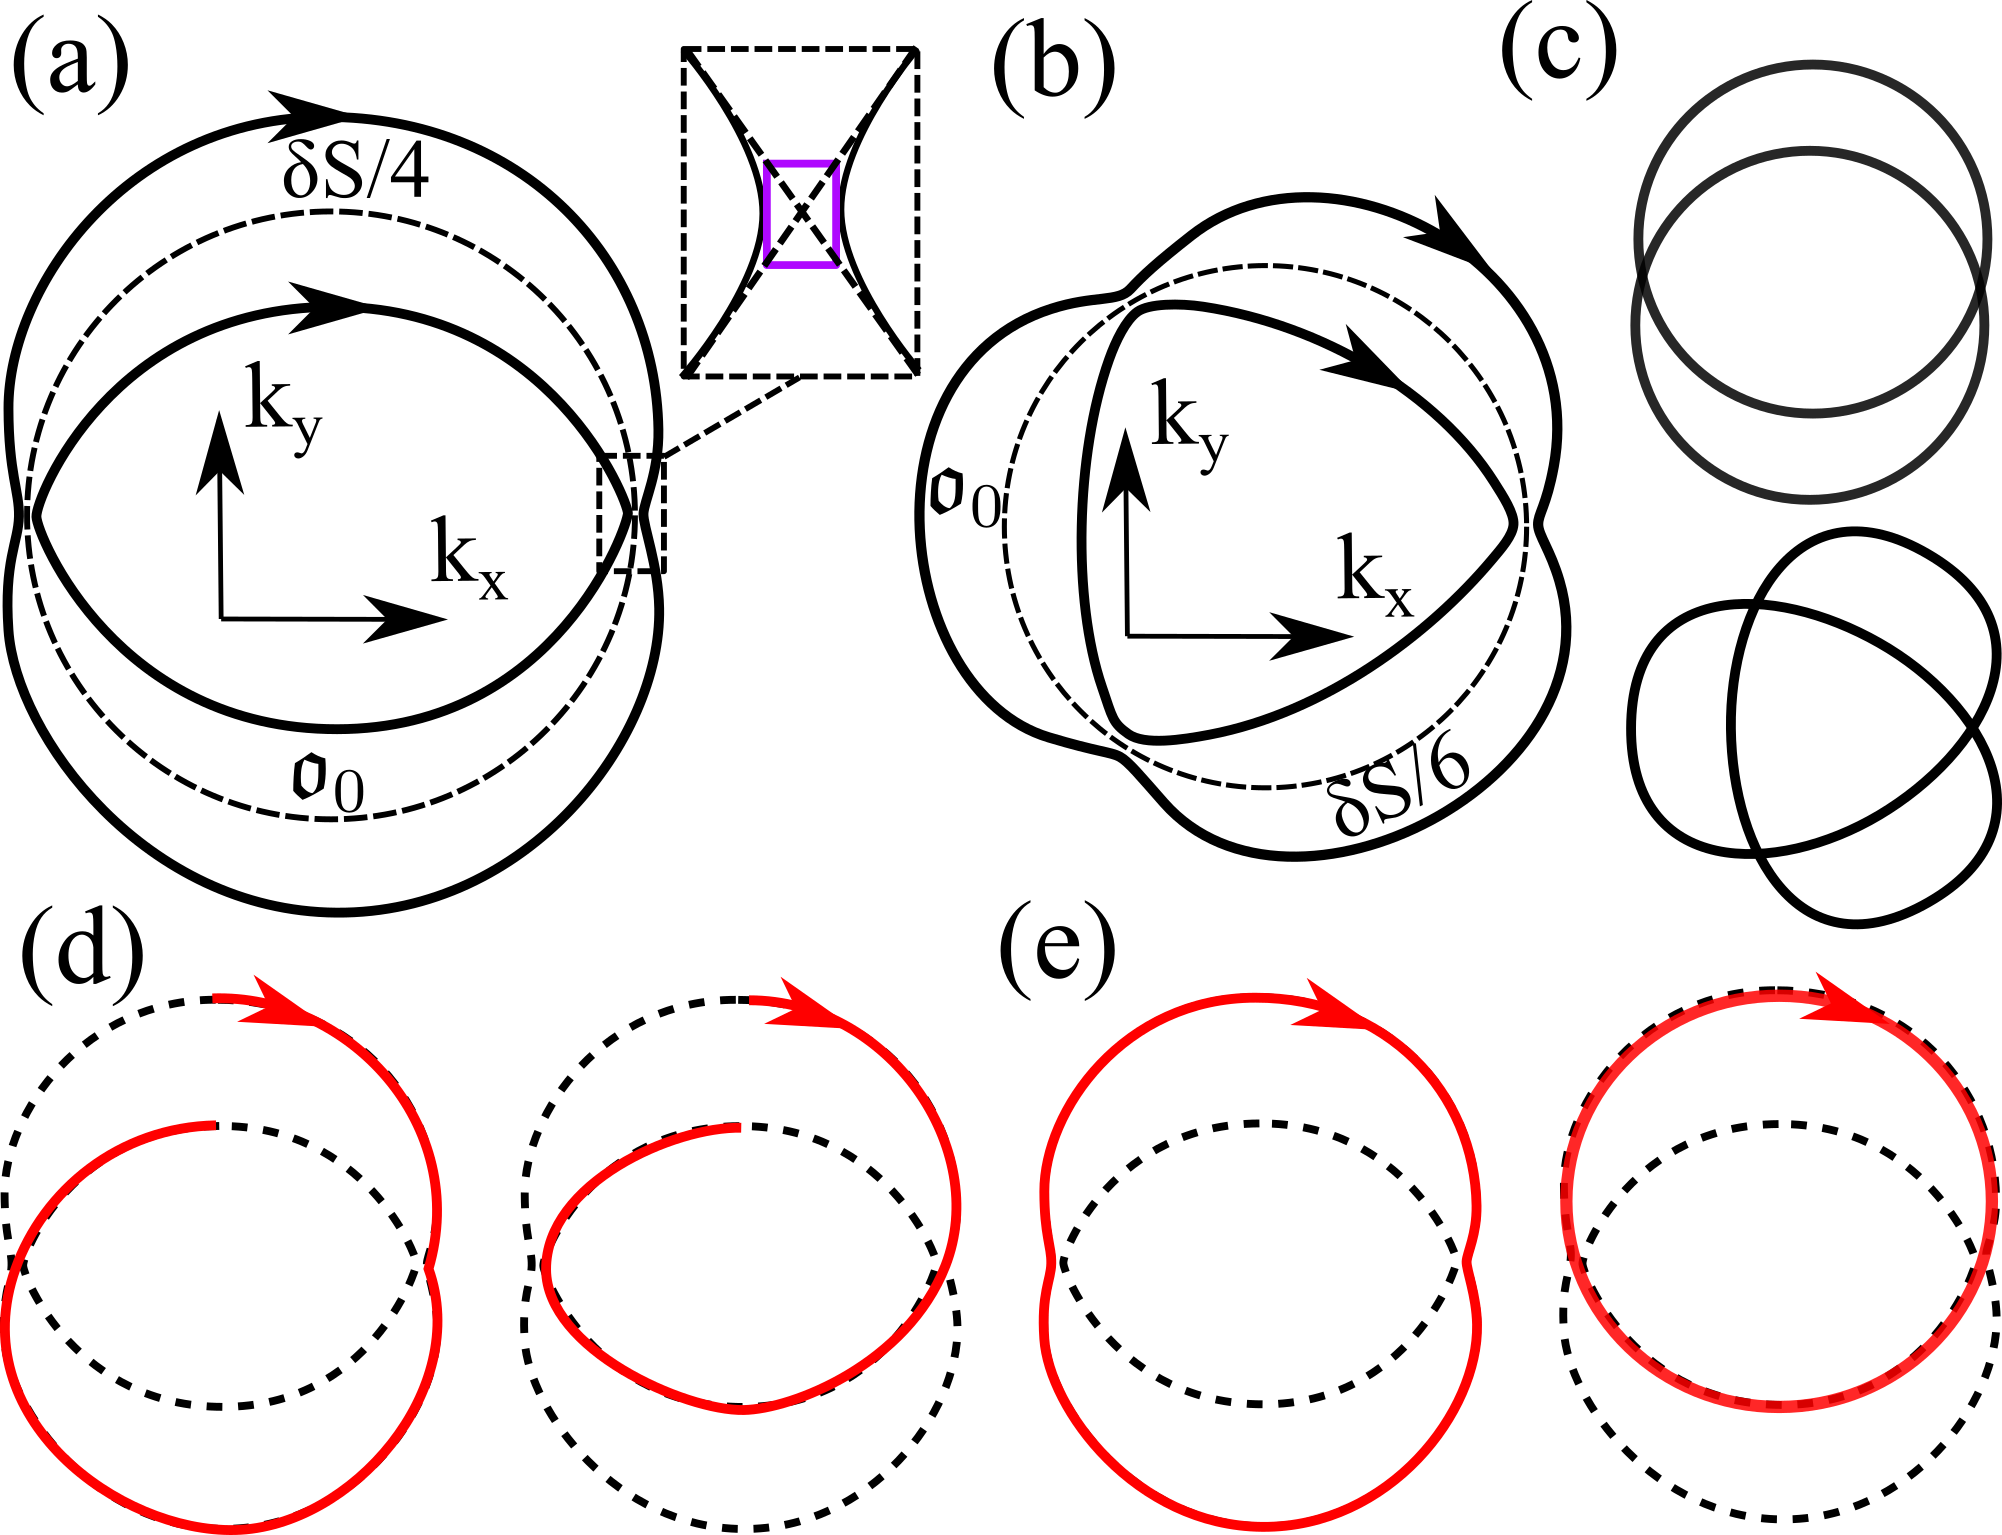
\includegraphics[width=1.0\columnwidth]{Cn-breakdown.png}
\caption{Cyclotron orbits for $\mathfrak{c}_2$-symmetric [(a)] and $\mathfrak{c}_3$-symmetric [(b)] breakdown. Top right inset of (a) presents an enlarged view of the breakdown junction, where the purple rectangle has area $S_{\sma{\square}}$. (c) Klein tunneling limit of $\mathfrak{c}_2$-symmetric (upper) and $\mathfrak{c}_3$-symmetric (lower) breakdown cyclotron orbits. (d) Two Feynman paths that switch to the other band by one tunneling event. (e) Two Feynman paths that returns to the same band by zero or two tunneling events. \label{fig:Cn-breakdown}}
\end{figure}


In the adiabatic limit of two quasidegenerate orbits, we have found [in \s{sec:introducecodimension}] that the codimension for $\cala{=}{\pm} I$ is unity. Here we investigate how this result changes as adiabaticity is relaxed by Landau-Zener tunneling -- that respects a discrete $N$-fold rotational symmetry ($\mathfrak{c}_N$). Since a II-Dirac cone is tilted in a special direction, a II-Dirac point cannot be the center of a rotational symmetry; the minimal model with $\mathfrak{c}_N$ symmetry thus requires $N$ distinct but symmetry-related II-Dirac points. For $N{=}2$, we will demonstrate that the codimension for $\cala{=}I$ (but not for $\cala{=}{-}I$) remains unity, in accordance with the symmetric-coordinate analysis of \q{proprashba}; the persistence of  Landau-level quasidegeneracies  (at finite tunneling probability) will be demystified in terms of the destructive interference of tunneling Feynman paths. For $N{=}3$, we will find that two of three Landau-level quasi-crossings are perturbatively stable against tunneling, but even these will destabilize beyond a critical tunneling strength.


%Quasidegenerate orbits feature tunneling everywhere along the cyclotron orbit and therefore demand a quantization rule that incorporates both tunneling and single band evolution of wave packets. Sometimes, the coherent evolution of wave packets and tunneling can be decoupled in the quantization rule in weak field limit, as exemplified by magnetic breakdown in Rashba-Zeeman model in Sec. \ref{sec:inplanezeeman}. Let us further explore single-parameter tunability of Landau-level quasidegeneracies in this limit by introducing a rotational symmetric Hamiltonian with isolated breakdown junctions at several isolated $\bk$ points. Besides being an interesting toy model, this Hamiltonian provides some insights of stability of Landau-level quasidegeneracies by perturbing from two otherwise independent orbits.

%For simplicity, we interpret the Pauli matrices as  spin operators, and the two right-most terms of  \q{modelC2breakdown} as a spin-orbit coupling.

We begin with a minimal, $\mathfrak{c}_2$-symmetric model:
\e{H=\f{{\hbar^2}k^2}{2m_1}+ \bigg(\f{{\hbar^2}k^2}{2m_2}-\mu\bigg)\sigma_z +wk_y\sigma_x,\label{modelC2breakdown}}
with $0{<}m_1{\ll}m_2$ and positive $\mu$.  The $\mathfrak{c}_2$ symmetry manifests as $\sigma_z H(\bk)\sigma_z{=}H({-}\bk)$, and relates 
two Dirac points at
\e{\bar{k}_x = \pm\sqrt{2m_2\mu}/{\hbar},\;\bar{k}_y=0,\;\epsilon_{0}=\frac{m_2}{m_1}\mu.}
In the vicinity of either point, the  Hamiltonian has the linearized form 
\e{H_{\pm} =\pm {\hbar}\sqrt{\f{2\mu}{m_2}}\bigg(\frac{m_2}{m_1}+\sz\bigg)\delta k_x+w\delta k_{y}\sx+\epsilon_0, \label{linearHam2}}
from which we deduce that both Dirac points are  type-II if $m_1{<}m_2$; we further assume $m_1{\ll}m_2$ so that the quasidegeneracy condition ($\delta S/S{\ll}1$) is satisfied. 

%this condition is henceforth assumed.\footnote{Actually we will impose the stronger condition $m_1{\ll}m_2$, to ensure that the relative change in band velocity (due to the spin-orbit coupling) is small. This is a consistency requirement of our WKB theory, as explained in \app{app:quantizationruleproof}.} 

%; near each point the orbits are well approximated by two hyperbolic arms
%$\phi_j{=}\int_{\sma{0}}^{\sma{T_c}}\calh_{jj}dt/\hbar$ is simply the cyclotron integral of the corresponding diagonal element of the effective Hamiltonian. 

% In the weak-field regime where $\var_c{=}{\hbar^2}/m_1l^2{\ll}\Delta$,




At energies close to the Dirac point ($E{-}\epsilon_0 {\ll} wm_2(2\epsilon_0/m_1)^{\sma{1/2}}$), there are two concentric orbits which (nearly) touch at both Dirac points, as illustrated in Fig. \ref{fig:Cn-breakdown} (a). For sufficiently weak field, interband tunneling is localized near either II-Dirac point, and occurs with the Landau-Zener probability:
\e{\rho^2=e^{-2\pi\bar{\mu}}, \; \bar{\mu}=\f{\big(Z_{\perp}^2+(m_1/m_2)^2(E-\epsilon_0)^2\big)l^2}{2w\sqrt{2E/m_1}}. \label{landauzenerc2}}
Equivalently, $\bar{\mu}{=}S_{\sma{\square}}l^2/8$, with $S_{\sma{\square}}$ the area of rectangle inscribed between the two hyperbolic arms [cf.\  Fig\ref{fig:Cn-breakdown}(a)]. Elsewhere, an electron undergoes adiabatic (band-conserving) dynamics. Due to $\mathfrak{c}_2$ symmetry, the time-evolution propagator over the full cyclotron period is simply the square of the propagator for half the period: 
\e{\A=\left(\matrixtwo{\tau e^{i\bar{\varphi}}}{-\rho}{\rho}{\tau e^{-i\bar{\varphi}}}{\diagmatrix{e^{i\tilde{\lambda}_-}}{e^{i\tilde{\lambda}_+}}} \right)^2. \label{propC2breakdown}}
The half-period propagator may be taken from \qq{scattmat}{propinplanezeeman}, with  $\bar{\mu}$ here given by \q{landauzenerc2}, and  $\tilde{\lambda}_{\pm}{=}{\pm}l^2\delta S/4$ plus a field-independent geometric phase.
 


%For the upper half ($k_y{>}0$) of Fig. \ref{fig:Cn-breakdown}(a), this adiabatic evolution is described by a diagonal unitary matrix in the basis of energy bands; the phase of the diagonal entry $\tilde{\lambda}_{\pm}{=}{\pm}l^2\delta S/4$ plus a field-independent geometric phase.  The time-evolution propagator  describes the time-ordered, coherent process of Landau-Zener tunneling/transmission (as described by the scattering matrix of \q{scattmat}) and adiabatic dynamics:

%The two scattering matrices for both Dirac points are identical by $\mathfrak{c}_2$ symmetry; so are the two diagonal propagators corresponding to the left and right halves of the adiabatic dynamics. 

% \footnote{due to this field-independent phase, it is not necessary that $\delta\lambda_+=-\delta\lambda_-$}


The necessary and sufficient condition for a degeneracy of $\cala$ is 
\begin{align}
\Delta:= \tilde{\lambda}_-{-}\tilde{\lambda}_{+}{+}2\bar{\varphi},\;\;
\tau\cos\f{\Delta}{2}= \begin{cases} 0, & {\A}=+I \\
                 \pm 1, & \A =-I\end{cases}.\label{c2breakdowndgncondition}
\end{align}
$\Delta$ is the differential phase between two Feynman paths  that involve a single tunneling event  over one cyclotron period, as illustrated in Fig. \ref{fig:Cn-breakdown}(d).
The adiabatic limit is given by $\tau{=}1$ and $\bar{\varphi}{=}0$, which leads to the satisfaction of \q{c2breakdowndgncondition} for $l^2$ equal to an integer multiple of $2\pi/\delta S$ up to a field indepedent offset. As noted in \s{sec:introducecodimension}, such a periodicity corresponds to a differential increment of a single, magnetic flux quantum. 

Deviating from the adiabatic limit, we deduce from \q{c2breakdowndgncondition} that  $\A{=}I$ remains attainable by varying $B$, but $\A{=}{-}I$ is unattainable because $\tau{<}1$; this is consistent with the codimension analysis of \q{proprashba}. The conditions $\A{=}I$ and $\rho{>}0$ are interpreted as the destructive interference of  two, single-tunneling Feynman path (cf. Fig. \ref{fig:Cn-breakdown}(d)). Concurrently, there is constructive interference of the Feynman loops involving zero and two tunneling events (cf. Fig. \ref{fig:Cn-breakdown}(e)). The differential phase between outer and inner zero-tunneling (band-conserving) loops is simply 0 (mod $2\pi$), hence Landau levels are quasidegenerate. Such quasidegeneracies recur as $\Delta$ advances by $2\pi$, corresponding to a periodicity in $l^2$ of $4\pi/\delta S$ (or two flux quanta). This periodicity is not affected by the additional phase $2\bar{\phi}$ in $\Delta$, because $\bar{\phi}$ varies on the scale  $2\pi/S_{\sma{\square}}$,\footnote{For $\bar{\varphi}(\bar{\mu})$ to vary  $\sim 1$, the Landau-Zener parameter $\bar{\mu}$ must vary by $\sim 1$ [cf.\  Fig.\ 10 in 100page]. Moreover, $2\pi\barmu{:}{=} (2\pi/8) l^2S_{\sma{\square}}$.[AALG]} which is much larger than $4\pi/\delta S$. To recapitulate, half the Landau-level quasi-crossings (over the $B$ axis) are destabilized  by tunneling; the robustness of the other half relies on $\mathfrak{c}_2$ symmetry. There exists a complementary argument for the existence of Landau-level quasi-crossings in the Klein-tunneling limit $(\tau{=}0)$: the two independent orbits are related by $\mathfrak{c}_2$ symmetry, leading to exactly-degenerate Landau levels.  


%The degeneracies alternate between $\cala{=}I$ and ${-}I$ on the B axis, hence the subset of degeneracies corresponding to $\cala{=}I$ (or ${-}I$) occur with a period of  $4\pi/\delta S$ (or two flux quanta).  

%occurs if and only if $\rho{=}0$ and  $\exp[i(\delta \lambda_+{+}\bar{\varphi})]$ is real, while 


%Let us investigate the fate of these degeneracies as $\rho$ increases. While asymmetric interband tunneling generically destabilizes all degeneracies, we will demonstrate that two-fold-symmetric interband tunneling destabilizes only half of them. Indeed, 


%for $\rho{>}0$, only 0 in Eq. (\ref{c2breakdowndgncondition}) is possible, destabilizing half of the degeneracies. \footnote{Notice cosine function reaches 0 twice in a period}

%Eq. (\ref{c2breakdowndgncondition}) with $0$ on the right hand side is the condition for destructive interference of the two Feynman paths that contribute to interband tunneling (as illustrated in \red{[Fig]}); this occurs with a period  of   $4\pi /\delta S$ (or two flux quanta). 


%$2\pi\bar{\mu}{\sim}l^2 S_{\sma{\square}}/8$ where $S_{\sma{\square}}$ is much smaller than $\delta S$ [see inset of Fig. \ref{fig:Cn-breakdown}(a)].





%The periodicity (in $l^2$) of the destructive interference has a dual interpretation  in real space -- as a periodic increment of \textit{two} flux quanta for  the differential magnetic flux (between the two spin-split orbits).\footnote{To clarify, band-conserving orbits do not generically describe the dynamics -- except at fine-tuned fields associated to destructive interference of interband tunneling.} 


%This  provides yet another  illustration of the general statement proposed in \s{sec:singleparameterrashba}: due to two-fold rotational symmetry, half the degeneracies have unit codimension, and the other half has codimension two. 


For our last illustration, we consider a II-Dirac model with $\mathfrak{c}_3$  symmetry, as   illustrated in Fig. \ref{fig:Cn-breakdown}(b). In the adiabatic regime ($\tau{\approx}1$), Landau-level quasidegeneracies occur with a periodicity of one flux quantum; however, in the Klein-tunneling regime ($\tau{\approx}0$), there exists only one dominant orbit shaped like a three-fold-symmetric trefoil knot --  all Landau levels are nondegenerate with spacing determined by the effective mass of the trefoil; this property generalizes to $\mathfrak{c}_N$-symmetric II-Dirac models with odd $N$.   

To resolve this tension (for $N{=}3$), consider that the propagator $\A$ has a form analogous to \q{propC2breakdown} -- but with $(\cdot)^2$ replaced by $(\cdot)^3$, and with $\tilde{\lambda}_\pm{=}{\pm} l^2\delta S/4$ replaced by $\pm l^2\delta S/6$ (plus a field-independent geometric correction). The degeneracy condition is modified to $\tau\cos[(\tilde{\lambda}_+{-}\tilde{\lambda}_-)/2{+}\bar{\varphi}]{=}{\pm} 1,{\pm} 1/2$. With nonzero tunneling ($1/2{<}\tau {<}1$), only $\pm 1/2$ is attainable -- this implies that of every three degeneracies that exist in the adiabatic limit, only two are perturbatively stable. Beyond a critical field  (defined by $\tau{=}1/2$), all degeneracies coalesce pairwise (on the $B$ axis) and annihilate. 

We conclude this section with a general result that is valid for any integer $N{\geq}2$: of every $N$ quasi-crossings that exist in the adiabatic limit, $N{-}1$ of them are perturbatively stable against tunneling that respects  $\mathfrak{c}_N$ symmetry. We prove this in App. \ref{app:codimension}.

\textbf{[Bonus: A different realization of two-fold symmetric breakdown: angular magnetoresistance oscillations.]}

\subsection{The ten-fold table for symmetry constrained codimensions}\label{sec:tenfold}

\begin{table*}
\begin{tabular*}{\textwidth}{c@{\extracolsep{\fill}}ccccccc}
\hlineB{2.0}
             class number & action on orbit & action on $\bk$ & $u$ & $s$ & quasidegenerate & $g$ & codimension\\
\hline
\multirow{2}{*}{1} & \multirow{10}{*}{$|g\circ \frako_0| = |\frako_0|$} & \multirow{4}{*}{$\forall \bk \in \frako_0$, $g\circ \bk=\bk$} & \multirow{2}{*}{0} & \multirow{2}{*}{0} & \multirow{2}{*}{$\surd$} & $\breve{g}\propto I$ & 3  \\
 & & & & & & $\breve{g}\not\propto I$ & 1 \\
 \cline{4-8}
\multirow{2}{*}{2} & & & \multirow{2}{*}{0} & \multirow{2}{*}{1} & & $g^2=1$ & 1  \\
 & & &  &  & & $g^2=-1$ & 3  \\
 \cline{3-8}
3 & & \multirow{6}{*}{$\exists \bk \in \frako_0, g\circ \bk\ne\bk$} & 0 & 0 & $\surd$ & - & 1   \\
\cline{4-8}
4 & & & 0 & 1 & & - & 1   \\
\cline{4-8}
\multirow{2}{*}{5} & & & \multirow{2}{*}{1} & \multirow{2}{*}{0} & & $\breve{g} \propto \sigma_z$ & 2  \\
 & & & &  & & $\breve{g} \not\propto \sigma_z$ & 0  \\
\cline{4-8}
\multirow{2}{*}{6} & & & \multirow{2}{*}{1} & \multirow{2}{*}{1} & \multirow{2}{*}{$\surd$} & $g^2=1$ & 2  \\
& & & &  & & $g^2=-1$ & 0  \\
\hline
7 & \multirow{4}{*}{$|g\circ \frako_0| \ne |\frako_0|$} & \multirow{4}{*}{-} & 0 & 0 & $\surd$ & - & 3 \\
\cline{4-8}
8 &  &  & 0 & 1 & & - & 3 \\
\cline{4-8}
9 &  &  & 1 & 0 & & - & 3 \\
\cline{4-8}
10 &  &  & 1 & 1 & $\surd$ & - & 3 \\
\hlineB{2.0}
\end{tabular*}
\caption{Symmetry-constrained codimensions for the two-by-two propagator $\A$. The first column numbers the symmetry class of $\A$. The second and third column defines how the symmetry acts on the cyclotron orbit. The next two columns  inform us if the mapping $\bk{\rightarrow}g{\circ}\bk$ [cf.\ \q{gmapk}]  preserves ($u{=}0$) or inverts ($u{=}0$) the orientation of the orbit, and if $g$ preserves ($s{=}0$) or inverts ($s{=}1$) the arrow of time. The sixth column indicates whether this  class is potentially a symmetry of quasidegenerate orbits. The seventh column specifies additional conditions (on the representation of $g$) which must be imposed to uniquely determine the codimension. $\breve{g}$ is defined as the diagonalized, unitary matrix representation of $g$ in the degenerate subspace of $\hat{H}_0$. In class 5, $\breve g$ is evaluated at $g$-invariant $\bk$ ($g\circ\bk=\bk$). For the reader's convenience, we present some commonly-used matrix representations for exactly degenerate bands in Tab.\ \ref{table:sewing-matrix}. The last column presents codimensions of the degeneracy manifold. For exactly-degenerate orbits in class 2, 4 and 5, $\A$ satisfies $\text{det}(\A){=}1$,[topofermi] with the assumption that spin-orbit coupling can be turned off continuously without changing the degeneracy of the orbit. 
 \label{table:codimension}}
\end{table*}

Generalizing our rotational-symmetric case studies in
Sec.\ \ref{sec:singleparameterrashba}-\ref{sec:rotsymmbreakdown}, we now present the symmetry-constrained codimensions for all ten[topoferm] symmetry classes of orbits. Depending on the class, the codimension is either $0,1,2$ or $3$. We begin by briefly reviewing the ten-fold symmetry classification of orbits in \s{sec:reviewtenfold}. We then study in Sec. \ref{sec:codimquasideg} five of the classes which is relevant to quasidegenerate orbits. The remaining five classes are relevant to exactly degenerate orbits, which we study in Sec. \ref{sec:codimexactdeg}.

\subsubsection{Ten-fold classification of orbits}\label{sec:reviewtenfold}

%%We restrict our attention to the subset of $g$ (in the space group) that preserves all field-orthogonal $\bk$-planes, where  orbits  are confined.\textbf{[might say something different about 2DEG]}


Any symmetry $g$ of a field-independent, translation-invariant Hamiltonian $\hat{H}$ acts on space-time as
\begin{align}
&g: \vectwo{\br}{t} \rightarrow \matrixtwo{\check{g}}{0}{0}{ (-1)^{s(g)}}\vectwo{\br}{t}+\vectwo{\bdelta}{0}, \label{definesg}
\end{align}
with $s(g){=}0$ (resp.\ $1$) if $g$ preserves (resp.\  reverses) the arrow of time. $\check{g}$ is the matrix representation of $g$ in real space, and the corresponding action of  $g$ on the crystal wavevector is  
\e{\bk \rightarrow g\circ\bk := (-1)^{s(g)}\check{g}\bk. \label{gmapk}}
Given $\hat{H}$ and the orientation of the magnetic field, electrons follow orbits (denoted $\frako$) that are confined to field-orthogonal $\bk$-planes.  Given an orbit $\frako$, we restrict our attention to the subgroup of $\hat{H}$ that maps the orbit to itself (denoted as $|g\circ\frako|{=}|\frako|$) or to a distinct orbit ($|g\circ\frako|{\ne}|\frako|$). In the former mapping, we may further distinguish two cases: (a)  $g$ maps every $\bk$ on the orbit to itself, as exemplified by the composition $T\inv$ of time reversal ($T$) and spatial inversion ($\inv$)  symmetries. (b) There exists at least one $\bk$ on the orbit that is mapped to a distinct wavevector, e.g., time-reversal symmetry relates two wavevectors ($\bk$ and ${-}\bk$) on an orbit that encircles a time-reversal-invariant point. 

Lastly, we distinguish  between mappings [\q{gmapk}] that preserve  ($u(g){=}0$) or invert ($u(g){=}1$) the orientation of the orbit. For example, a rotation with axis parallel to the field is orientation-preserving, while a reflection with axis orthogonal to the field is orientation-inverting. The combination of all distinguishing criteria leads to   a ten-fold classification of orbits $\frako_0$ with $g$ symmetry, as was first presented in [topoferm] and is summarized by the ten numbered rows in \tab{table:codimension}.
 
 

%In the latter case there exists no self-constraint on the propagator $\A$ [cf.\ \q{eq:prop}] due to $g$ alone, hence the codimension 


% preserves  ($u(g)=0$) or inverts ($u(g)=1$) the orientation of the orbit. In the latter case ($|g\circ\frako_0|\ne|\frako_0|$), no constraint exists between $\A$ and itself
 

\subsubsection{Symmetry-constrained codimension for quasidegenerate orbits}\label{sec:codimquasideg}


In the particular context of quasidegenerate bands, $\hat{H}{=}\hat{H}_0{+}\delta \hat{H}$ is the sum of a zeroth-order Hamiltonian (with spin-degenerate bands) and a symmetry-lowering perturbation.  Given a zeroth-order orbit $\frako_0$ of $\hat{H}_0$, we  are interested in the subgroup of $\hat{H}$ that  maps $\frako_0$ to itself or to a distinct zeroth-order orbit. 

Of the ten classes described in \s{sec:reviewtenfold}, only five   are relevant to quasidegenerate orbits (which are split with differential area  $\delta S$ that is much less than the area of $\frako_0$).
To identify this five, recall that the subleading corrections to our quantization rule are determined by the propagator $\A$ [cf.\ \q{eq:prop}], which is a time-ordered exponential of an effective Hamiltonian $\H{=}\delta\epsilon{+}B \mathcal{M}$ [cf.\ \q{eq:H1}]; $\H$ perturbatively encodes $\delta H$ and the Zeeman interaction, for an electron travelling over  $\frako_0$. Since $g$ is  a symmetry of  $\delta \hat{H}$, $\delta\epsilon$ is invariant under action of $g$. On the other hand, $\mathcal{M}$ is the field-parallel component of a pseudovector that is odd under time reversal,[sakurai] hence changes under $g$ to  $(-1)^{u+s}\mathcal{M}$  (plus a gauge-dependent term[100page] which is not essential to the present argument). Only with $u{+}s{=}0$ or $2$ would both terms in $\H$ transform consistently (invariantly) under $g$ -- this identifies the five ticked classes in Tab.\ \ref{table:codimension}.


%\textit{quasidegenerate} orbits; such orbits are split with differential area  $\delta S$ that is much less than the area of the zeroth-order orbit $\frako_0$. We remind the reader that $\frako_0$ is determined from the field orientation and the spin-degenerate bands of $\hat{H}_0$, while $\delta S$ is further determined by a symmetry-lowering perturbation: $\hat{H}{=}\hat{H}_0{+}\delta \hat{H}$.  

%To recapitulate the discussion in \s{sec:reviewtenfold}, we are interested in $g$ belonging to the subgroup of $\hat{H}$ that 
% maps $\frako_0$ to itself or to a distinct zeroth-order orbit. In the less-general context of quasidegenerate orbits, we shall impose additional restrictions that restrict $g$ to five of ten classes. 



For these five classes (labelled 1, 3, 6, 7 and 10 according to the first column of Tab.\ \ref{table:codimension}), we list their corresponding \textit{symmetry-constrained codimensions} in the right-most column of Tab.\ \ref{table:codimension}; these numbers are derived in  App.\ \ref{app:codimension}. To clarify, we define the $g$-constrained codimension as the minimal codimension -- among all degeneracy manifolds -- as enforced by $g$ symmetry. To motivate `minimal' in this definition, we have found that two-fold rotational symmetry reduces the codimension of the $\A{=}{+}I$ manifold (to unity), but not the codimension of the $\A{=}{-}I$ manifold [cf.\ \q{proprashba}]; the rotation-constrained codimension is then unity. Generally, it is only in class 3 and 4 that different  degeneracy manifolds may have different codimensions. Each entry in the right-most column of Tab.\ \ref{table:codimension} equals the $g$-constrained codimension for any $g$ in that class (and possibly satisfying an additional constraint on the representation of $g$, as specified by the second-to-last column).

Of the five classes only three (1, 3 and 6) potentially have symmetry-constrained codimensions that are reduced from three: these three have in common that  $|g\circ\frako_0|{=}|\frako_0|$, and therefore the propagator $\A$ [cf.\ \q{eq:prop}] is self-constrained. To clarify, a self-constraint relates  the propagator $\A$ [cf.\ \q{eq:prop}] to itself or to its inverse $\A^{-1}$, depending respectively on whether $u{=}0$ or $1$.  

%To uniquely determine the codimension in some classes,  conditions for the symmetry representation of $g$ must be specified: in class 1 for unitary $g$ that preserves the arrow of time ($s{=}0$),  

Class 1 groups together  spatial symmetries that preserve the arrow of time and map every $\bk$ on $\frako_0$ to itself. The simplest example is of $g$  a reflection symmetry with axis parallel to the field, and of  $\frako_0$ that is confined to a $g$-invariant $\bk$-plane. To uniquely determine the symmetry-constrained codimension in class 1, one must specify if the quasi-degenerate bands belong to identical or distinct representations of $g$.  The symmetry-constrained codimension is reduced to unity in the latter (and only the latter) case, due to the absence of level repulsion between distinct representations of $g$ -- the corresponding quasidegeneracies of Landau levels would then be exact degeneracies, rather than the near degeneracies described by \qq{llquasideg}{llquasidegB}.   

%we specify certain conditions on  $\breve{g}$, the \emph{diagonalized}, two-by-two matrix representation  of $g$; 

Class 3 corresponds to spatial symmetries that preserve the arrow of time and the orientation of $\frako_0$, as exemplified by rotational symmetry with rotational axis parallel to the field. The symmetry-constrained codimension here is unity, as has been modelled in Sec.\ \ref{sec:singleparameterrashba}-\ref{sec:rotsymmbreakdown}.

Symmetries in class 6 reverse both the arrow of time and the orientation of the orbit. The symmetry-constrained codimension is $2$ or $0$, depending respectively on whether the antiunitary representation of $g$ squares to $+1$ or $-1$. The former is exemplified by the composition $T\mathfrak{r}_{y=-x}$ of time reversal with a reflection symmetry (with reflection axis orthogonal to the field); this is a symmetry of the Rashba-Dresselhaus Hamiltonian [cf.\ \q{hamRD}]:
\e{ g H_{RD}(k_x,k_y)g^{-1} = H(k_y,k_x),\;\; g = e^{i\sigma_z\pi/4}K,}
with $K$ implementing complex conjugation. A consequence of this symmetry is that the degeneracy line node in Fig. \ref{fig:dgn}(b) is robust -- a property we had previously (and consistently) deduced from continuous rotational symmetry. An example of $g^2{=}-1$ is given by
the composition $T\mathfrak{r}_{x,\boldsymbol{c}/2}$ of time reversal with a glide symmetry; $\mathfrak{r}_{x,\boldsymbol{c}/2}$ is itself the composition of a reflection (with axis orthogonal to the field) and half a lattice translation (parallel to the field). The propagator for an orbit in the Brillouin-zone boundary ($k_z{=}\pi$ plane) would then be Kramers-degenerate -- the symmetry-constrained codimension vanishes.

%In the latter case, the codimension vanishes due to Kramers degeneracy. In the former case, the codimension is calculated to be 2, which is exemplified by $H_{RD}$ respecting $T\mathfrak{r}_{y=-x}$, with $\mathfrak{r}_{y=-x}$ being reflection transforming $x$ to $y$ and $z$ to $z$. 

%Therefore, codimension 2 in table \ref{table:codimension} instructs the degeneracy manifold in Fig. \ref{fig:dgn}(b) should be one dimensional, providing an alternative explanation of the line node in Fig. \ref{fig:dgn}(b).


%Extensively studied in Sec. \ref{sec:singleparameterrashba}-\ref{sec:rotsymmbreakdown} is class-3 (3rd row in the table), where rotational symmetry guarantees Landau level quasidegeneracy can be expected by tuning $B$ alone. Class-1 presents another example of codimension 1. Unitary symmetry in class-1 with $\breve{g}\not\propto I$ assigns different symmetry eigenvalues to the two degenerate bands (of $\hat{H}_0$) on $\frako_0$ and forbids hybridization between them. Therefore, $\A$ assumes a diagonal form and admits only one free variable. Class-1 symmetries with $\breve{g}\propto I$, acting effectively as identity operator, impose no constraints on $\A$ and thus no reduction in codimension.

%Codimension 0 is exemplified by class-6 with $g^2=-1$, where any eigenvector of $\A$ here is paired with another one due to Kramer's degeneracy. 





%\red{In our definition, $g$ is called a symmetry if $\hat{g}$ commutes with both $\hat{H}_0$ and $\delta \hat{H}$. Therefore, $\delta \epsilon$ is invariant under the action of $g$. For $\cal H$ to transform consistently under $g$, $g$ must preserve the magnetic moment $\mathcal{M}$. The magnetic moment is odd under time reversal, and behaves as a pseudovector under spatial transformations.[sakurai] Therefore, either (i) $g$ preserves the direction of time and is a proper transformation of space, or (ii) $g$ inverts the direction of time and is an improper transformation of space.} (i) is exemplified by a rotational symmetry with the rotational axis aligned parallel to the field, and (ii) by the composition  of time reversal $T$ and a spatial reflection $\mathfrak{r}_x$ (with reflection axis perpendicular to $\vec{B}$). 
%As discussed at the end of \s{sec:introducecodimension}, these classes either respect $u+s=0$ or $u+s=2$. \red{[These discussions moved to Sec. IV B]}





%$T\mathfrak{r}_{x,\boldsymbol{c}/2}$ ($\mathfrak{r}_{x,\boldsymbol{c}/2}$ is glide plane translating in $z$ direction for half a lattice vector after flipping $x$ direction) at $k_z=\pi$ is an example of codimension 0, corresponding to class-6 (the 6th class in the table)  with condition $g^2=-1$. Due to similar reasons as Kramer's degeneracy, Landau-level quasidegeneracy are guaranteed for arbitrary parameter choice. Rotational symmetry belonging to class-3 has codimension 1, as confirmed by numerical study and arguments in Sec. \ref{sec:singleparameterrashba} and \ref{sec:rotsymmbreakdown}. Codimension 2 is exemplified by $T\mathfrak{r}_x$ ($\mathfrak{r}_x$ is reflection in $x$ direction) belong to class-6 with $g^2=1$. Class-1 symmetries with $\breve{g}\propto I$, acting effectively as identity operator, imposes no constraints on $\A$ and thus no reduction in codimension.

%\red{[need to define stable or robust]} Codimension 1 does not imply every degeneracy is robust, which is a stronger statement than degeneracy manifold can be found by tuning a parameter. If degeneracy manifold contains distinct components of different codimension, every degeneracy being robust implies all these components having codimension 1, which is generally not the case, as exemplified by rotational symmetry discussed in Sec. \ref{sec:singleparameterrashba} and \ref{sec:rotsymmbreakdown}. Table \ref{table:codimension} only lists the smallest codimension, which is the number of parameters needed to find a degeneracy. 

%We end this section by a general discussion of free parameters that is most tunable in experiments. In transport experiments, magnetic field $B$ is generally tunable; in tunneling spectroscopy experiments, both $B$ and bias voltage $E$ is tunable. If codimension of degeneracy is 1, as constrained by two types of symmetries in Table \ref{table:codimension}, Landau level degeneracies can be found by tuning either $B$ or $E$. We have argued in Sec. \ref{sec:qtznrules} that $\lambda_a$ varies slowly with respect to $B$ and $E$. Hence an \textit{aperiodic} beating pattern is expected by tuning either $B$ or $E$.

\subsubsection{Symmetry-constrained codimension for exactly-degenerate orbits}\label{sec:codimexactdeg}

This work has mainly focused on the Landau quantization of quasidegenerate bands, which are eigenstates of the field-independent Hamiltonian $\hat{H}_0{+}\delta \hat{H}$. In this section we focus on higher-symmetry solids where the degeneracy-lifting perturbation $\delta \hat{H}$ is disallowed. $\hat{H}_0$ may or may not include spin-orbit coupling; in the former case, a crystalline point-group symmetry (e.g., $T\inv$ symmetry) is required for energy bands to be  two-fold degenerate at zero field.

Given $\hat{H}_0$ and the orientation of the field, electrons of opposite spin follow exactly-overlapping orbits (denoted $\frako_0$) which are confined to field-orthogonal $\bk$-planes. Such overlapping orbits will be referred to as \textit{exactly-degenerate}, in contrast with quasidegenerate orbits that are split on the $\bk$-plane. Despite the exact degeneracy of orbits, the corresponding Landau levels are generically split by the Zeeman interaction $B\calm$. We may therefore ask, in complete analogy: how many tunable parameters are required to attain a Landau-level (quasi)degeneracy for exactly-degenerate orbits? 


%The preceding codimension analysis may be straighforwardly extended to  energy bands that are exactly $D$-fold degenerate (at every wavevector) in the absence of the field. For simplicity we focus on $D{=}2$ spin degeneracy, which may arise in solids with negligibl\e spin-orbit coupling, and also in spin-orbit-coupled solids with certain crystallographic point-group symmetries (e.g., $T\inv$ symmetry).   


We answer this question in nearly the same vein as for quasidegenerate orbits: the quantization rule for exactly-degenerate orbits[topoferm] has the same form as \qq{eq:rule}{berryconn} with $\delta \var{=}\delta S{=}0.$ An eigenvalue-degeneracy of $\A$ would also imply a Landau-level quasidegeneracy, since the analysis of \s{sec:relatedegeneracies} applies to the special case $\delta S{=}0$. 

There is, however, a difference in the possible symmetry classes that apply to exactly-degenerate vs quasidegenerate orbits.  In \s{sec:codimquasideg}, we restricted ourselves to symmetries  that map the magnetic moment  $\calm$ to itself (plus a gauge-dependent term[100page]), so that both terms in $\calh{=}\delta \var{+}B\calm$ transform consistently as scalars. In the present context, this restriction is void because $\delta\var{=}0$, hence we \textit{also} allow for symmetries that invert the sign of $\calm$. 

Some $\calm$-inverting symmetries also exhibit reduced symmetry-constrained codimensions, as listed in the five \textit{unticked} classes of \tab{table:codimension}. As a case in point, class-2 symmetries invert time and $\calm$, and map  every wavevector (in $\frako_0$) to itself. The corresponding codimension is three (resp.\ one) if $g$ squares to $-1$ (resp.\ $+1$). The former is exemplified by $T\inv$ symmetry, and the latter by $T\rot_{2z}$ (the composition of time reversal with a two-fold rotation about the field direction). For an exactly-degenerate orbit $\frako$ confined to a $\rot_{2z}$-invariant plane, the associated propagator $\A$ is unitarily equivalent to a special orthogonal matrix [AA,100page] with a single, tunable angle of rotation -- this provides an intuitive explanation for the unit codimension.

%the angle of rotation associated to any SO(2) matrix then provides the single tuning parameter.

The simplest example of codimension reduction by a $\calm$-preserving symmetry is that of continuous spin-rotation. This is a symmetry of any solid with negligible spin-orbit coupling, and results in the absence of Landau-level repulsion between different spin species [cf.\ unit symmetry-constrained codimension in class I, with non-identical symmetry eigenvalues]. In this case the Landau-level degeneracy is exact.  

The detailed modelling of all ten classes of exactly-degenerate orbits is left to future work. We conclude this section by commenting on the tunable experimental parameters that are relevant to exactly-degenerate orbits. The absence of $\delta\var$  implies that the eigenvalues of $\cala$ are independent of the magnitude of $B$ [cf.\ \q{lambdasmallB} with $\delta S{=}0$]. However, the generic anisotropy of $\calm$ (viewed as a pseudovector) suggests that we may sweep the orientation of $B$; the generic energy-dependence of $\calm$ suggests that we may tune the bias voltage in tunneling spectroscopy.

%As derived in App.\ \ref{app:codimension}, 

%Absent this restriction, all ten symmetry classes may potentially apply to exactly-degenerate orbits, but only six of ten (with $|g\circ\frako_0|{=}|\frako_0|$) may have a symmetry-reduced codimension. The codimensions for three of these six classes have been explained in \s{sec:codimquasideg}, so here we focus on the other three.

%Landau level quasidegeneracy is not limited to quasidegenerate bands. For degenerate bands, a similar definition is applicable: \red{[need to check]}
%\e{ \f{E_{1}-E_2}{\var_c}\bigg|_{\bar{B}} = O\left(\f{\var_c}{E} \right). } 

%Landau levels of degenerate bands are characterized by a propagator $\A'$ similar to Eq. (\ref{eq:prop}) [100p]. Codimension analysis can be carried out similarly and the results are presented in table \ref{table:codimension}. 

%Unlike $\A$, all ten classes of symmetries impose constraints on $\A'$ and thus entries not applicable to $\A$ are useful for $\A'$.



%We have assumed in the above sections that the two-fold quasidegeneracy is due to small SOC. More generally, two-fold degenerate bands can be perturbed into quasidegenerate bands by symmetry breaking. From this viewpoint, our previous assumption of small SOC breaks continuous spin rotational symmetry which protects the degeneracy of spin up and spin down states. Other common symmetry operations capable of protecting two fold degeneracy are $T\mathfrak{i}$ and $T\mathfrak{c}_{2z,\boldsymbol{c}/2}$ at $k_z=\pi$, where $T$ is time reversal symmetry; $\mathfrak{i}$ is inversion symmetry and $\mathfrak{c}_{2z,\boldsymbol{c}/2}$ is two-fold screw rotation in $z$ direction. Table \ref{table:codimension} is applicable to quasidegenerate bands ($\A$) perturbed from degenerate bands protected by all the three symmetries and degenerate bands ($\A'$) due to $T\mathfrak{i}$ or $T\mathfrak{c}_{2z,\boldsymbol{c}/2}$. For degenerate bands protected by continuous spin rotation, codimension is at most 1 since $\A'$ is diagonal in spin basis. Codimension analysis without assumption of degenerate bands being protected by the three symmetries are presented in App. \ref{app:codimension}, where codimensions of Landau level quasidegeneracy for possibly fine tuned degenerate/quasidegenerate bands can be found.

\begin{table}
\begin{tabular*}{\columnwidth}{c@{\extracolsep{\fill}}ccc}
\hlineB{2.0}
class No. & symmetry  & origin of degeneracy & $\breve{g}\propto$ \\
\hline 
\multirow{2}{*}{1} & \multirow{2}{*}{$\mathfrak{r}_z$, $\mathfrak{r}_{z,\boldsymbol{a(b)}/2}$} & $T\mathfrak{i}$, spin SU(2) & $\sigma_z$ \\
\cline{3-4}
 & & $T\mathfrak{c}_{2z,\boldsymbol{c}/2}$ & $I$ \\
\hline
\multirow{3}{*}{5} & $\mathfrak{r}_{x(y),\boldsymbol{c}/2}$ & $T\mathfrak{i}$, spin SU(2), $T\mathfrak{c}_{2z,\boldsymbol{c}/2}$ & $\sigma_z$ \\
\cline{2-4}
& $\mathfrak{r}_{x(y)}$,$\mathfrak{r}_{x(y),\boldsymbol{b(a)}/2}$, & $T\mathfrak{i}$, spin SU(2) & $\sigma_z$ \\
\cline{3-4}
& $\mathfrak{c}_{2x(y)}$, $\mathfrak{c}_{2x(y),\boldsymbol{b(a)}/2}$ & $T\mathfrak{c}_{2z,\boldsymbol{c}/2}$ & $I$\\
\hlineB{2.0}
\end{tabular*}
\caption{Matrix representations of reflections (e.g., $\mathfrak{r}_x$) and rotations (e.g. $\mathfrak{c}_{2y}$) followed by possible half a lattice translations in $x,~y,~z$ directions (labeled by $\boldsymbol{a,~b,~c}$ respectively). This table is relevant for magnetic field in $\pm z$ direction. The two-fold exact degeneracy are assumed to be protected by either spatial-time inversion symmetry ($T\mathfrak{i}$), composition of time reversal and nonsymmorphic two fold rotation symmetry ($T\mathfrak{c}_{2z,\boldsymbol{c}/2}$) at $k_z=\pi$ or spin SU(2) (i.e., negligible SOC). \label{table:sewing-matrix}}
\end{table}


\section{Quantum-oscillatory phenomena for exactly- and quasi-degenerate orbits}\label{sec:qo}

In \s{sec:qtznrules} we have presented a quantization rule [\qq{eq:rule}{berryconn}] that is applicable to both quasidegenerate ($0{<}\delta S{<}S$) orbits and exactly-degenerate ($\delta S{=}0$) orbits. This section explores the implication of this rule for quantum-oscillatory phenomena of the Schubnikov-de Haas (SdH) [SdH] and de Haas-van Alphen (dHvA) [dhva] types. In \s{sec:quantosc_equidis}, we present a generalized Lifshitz-Kosevich formula that inputs our rule and outputs quantum oscillations. Applying this formula in the high-temperature regime, we will prove that  destructive interference of the fundamental quantum-oscillatory harmonic may  be tuned by at most one parameter in any symmetry class; this parameter may be the magnitude ($B$) of the magnetic field for quasidegenerate orbits, but not for exactly-degenerate orbits. \s{sec:quantosc_quasideg} focuses on the low-temperature SdH effect for quasidegenerate orbits in symmetry classes 1 to 4 [cf.\ \tab{table:codimension}], wherein we predict a smooth crossover from period-doubled to -undoubled oscillations upon variation of $B$ (at fixed particle density).




%In We have demonstrated for certain symmetry classes that Landau-level quasidegeneracies can be attained by tuning only the magnitude ($B$) of the magnetic field. This manifests in the Schubnikov-de Haas effect  as an aperiodic beating of the minima of conductivity (at fixed particle density), as described in \s{sec:quantosc_quasideg}. Analogously, it is also possible to attain quasi-equidistant Landau levels by tuning $B$; this manifests as an aperiodic, destructive interference of the fundamental quantum-oscillatory harmonic (at fixed chemical potential).


\subsection{Single-parameter tunability for the destructive interference of the fundamental harmonic}\label{sec:quantosc_equidis}

%and in the presence of magnetic breakdown [Kaganov, lifshitz];

Lifshitz-Kosevich formulae[lifshitzkosevich] allow for a harmonic analysis of quantum oscillations, and have previously been derived for  exactly-degenerate orbits in symmetry class 1[rothII], with the generalization to all ten symmetry classes in Ref. [topoferm]. A simple generalization of the derivation in [topoferm] extend the utility of these existing formulae to quasi-degenerate orbits of any symmetry. For example, the oscillatory component of the magnetization of 2D metals has the form
\begin{equation}
\delta M=-\frac{1}{2\pi}\frac{k_BT}{BS^{-1}}\sum_{a=1}^2\sum_{r=1}^{\infty}e^{-\f{r\pi}{\omega_c\tau_{\sma{D}}}} \frac{\text{sin}[r(l^2S{+}\lambda_a{+}\gamma)]}{\text{sinh}(2\pi^2rk_BT/\var_c)},\label{eq:LK}
\end{equation}
where the argument of the sine function involve quantities from our  quantization rule [\qq{eq:rule}{berryconn}]; $T$ is temperature and $\tau_{\sma{D}}$  the Dingle scattering lifetime. All the quantities on the right handside of Eq.\ (\ref{eq:LK}) are evaluated at the chemical potential. \q{eq:LK} corrects the analogous formula in Ref. [topoferm] by a factor of half. 

%For 3D metals, the oscillLifshitz-Kosevich formula is in a similar form, presented in Ref. [topoferm]. 

At high temperature ($kT{\gg}\var_c$) and/or with strong disorder ($\omega_c\tau_{\sma{D}}{\ll}1$), the dominant contribution to $\delta M$ is from the fundamental harmonic ($r{=}1$), which sums two sine functions with generically distinct phase offsets $\lambda_{1,2}$. This summation (or interference) is constructive if $\delta \lambda{=}|\lambda_1{-}\lambda_2|{\equiv}0$, and destructive if $\delta \lambda{\equiv}\pi$  ($\equiv$ denotes an equivalence modulo $2\pi$). In the latter case, only even-$r$ harmonics remain. 

%The former is associated to Landau-level quasidegeneracies, and the latter to quasi-equidistant Landau levels with spacing ${\approx}\var_c/2$.

We have shown in \s{sec:llquasideg} that  the number of tunable parameters required to attain  $\delta \lambda{\equiv}0$ ranges from $0$ to $3$; this number is a symmetry-dependent measure of Landau-level repulsion [cf.\ \tab{table:codimension}]. As illustrated in the right-most panel of Fig 7(b), $\delta \lambda{\equiv}\pi$ is the condition  for Landau levels to be quasi-equidistant  with spacing ${\approx}\var_c/2$; since no level repulsion need be overcome,
we expect $\delta \lambda{\equiv}\pi$ is attainable with at most one tunable parameter (in any symmetry class). To prove this, we return to the canonical parametrization of the SU(2) component (${\cal \bar{A}}$) of $\A$ [cf.\ \q{s3}]. The necessary and sufficient condition for $\delta \lambda{\equiv}\pi$ is that ${\cal \bar{A}}(r_1,r_2,r_3,r_4)$ has eigenvalues $+i$ and $-i$; the latter condition is equivalent to setting $r_1{=}0$ in \q{s3} -- a condition on a single parameter.\footnote{For an alternative proof,   $\delta \lambda{\equiv}\pi$ is equivalent to ${ \bar{\cal A}}{=}Ve^{i\sigma_z\pi/2}V^{-1}$ for some unitary $V\in U(2)$. The manifold associated to $\delta \lambda{\equiv}\pi$ is then the space of unitary matrices  that do not commute with $e^{i\sigma_z\pi/2}$.  The dimension of this manifold is the number of linearly-independent Hermitian generators (two) for unitaries that do not commute with $e^{i\sigma_z\pi/2}$. The codimension is then obtained from deducting two from the total number (three)  of linearly-independent Hermitian generators  for U(2). This approach of determining codimension is similar to that in [JHNR].} 

For exactly-degenerate orbits, the single parameter to attain destructive interference might be the chemical potential (as illustrated for the quantum oscillations of Na$_3$Bi in [topoferm]) or the orientation of the magnetic field; however $\lambda_a$ is independent of the field magnitude ($B$), as explained in \s{sec:codimexactdeg}. In principle, one may account for linear-in-$B$ corrections to $\lambda_a$ at stronger fields, however a quantitative theory for such corrections only exists (thus far) for non-degenerate orbits.[rothII,fischbeck,niu,fuchs] 

For quasidegenerate orbits,  $\lambda_a$ is expandable as a Laurent series in $B$ with leading term $1/B$ [cf.\ \q{lambdasmallB}], hence $B$ can be tuned to attain destructive interference. The slow variation of $\lambda_a$ compared to the action $l^2S$ [cf.\ \app{sec:slowvariation}] implies a beating pattern for the fundamental harmonic. In the weak-field, adiabatic regime, the antinodes of this pattern occur with period $2\pi/\delta S$ in $l^2$ [cf.\ \s{sec:introducecodimension}]; in the non-adiabatic regime, the antinodes are generically aperiodic [cf.\ \q{lambdasmallB}]. Such beatings have been observed for semiconductor heterostructures[das,several more]. Our contribution is the first semiclassical theory  [summarized by the quantization rule of \qq{eq:rule}{berryconn} and the Lifshitz-Kosevich formula of \q{eq:LK}] from which one can calculate the beating pattern; in particular, one may extract the intervals (in $1/B$) between antinodes  for the Rashba 2DEG [by imposing $\delta \lambda{\equiv}\pi$ in \q{eq:Rashba-lambda}] and for the Rashba-Dresselhaus 2DEG [see the next \s{sec:quantosc_quasideg}]. 

\begin{figure}
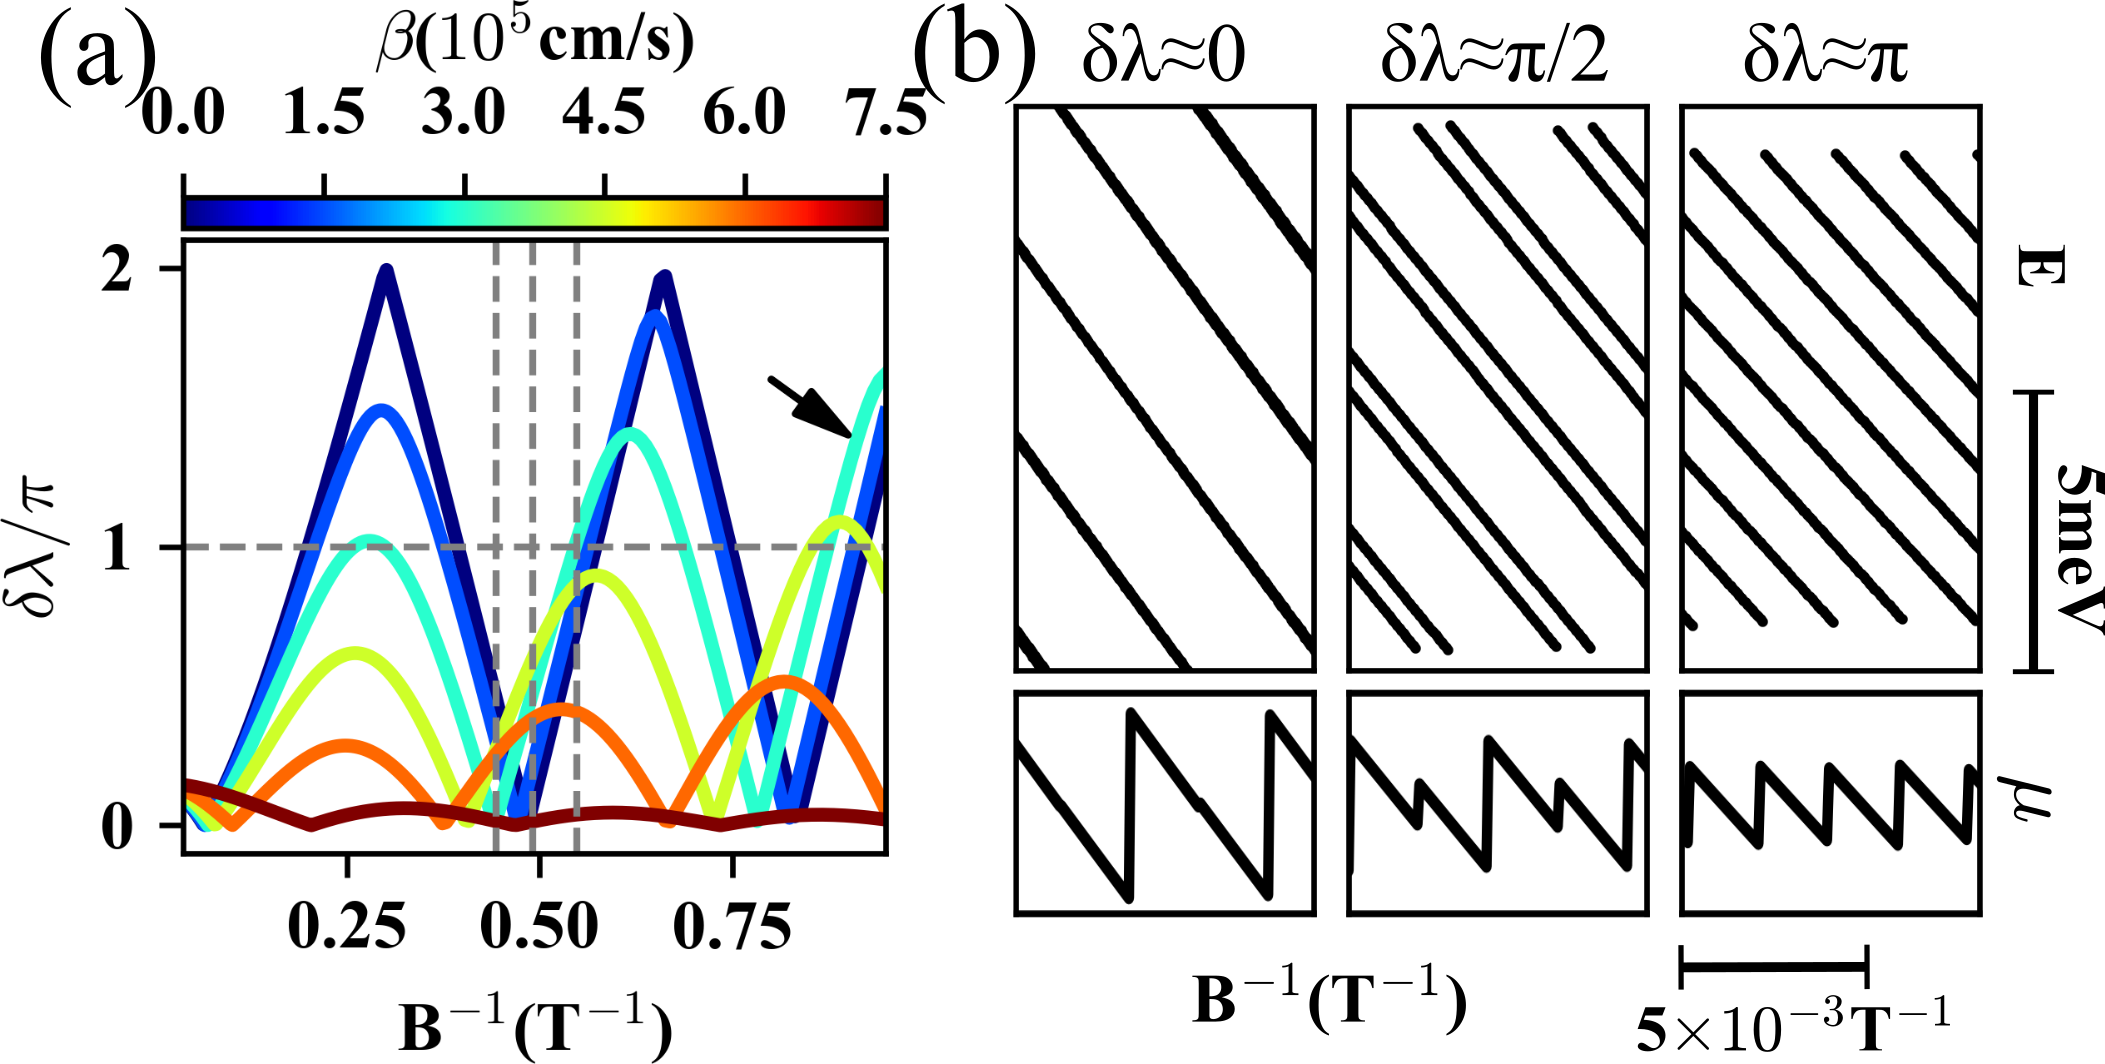
\includegraphics[width=1.0\columnwidth]{qo.png}
\caption{Quantum oscillations in the Rashba-Dresselhaus 2DEG. (a) Evolution of $\delta\lambda$ with respect to the inverse field for different values of $\beta$. The horizontal dashed line indicates $\delta\lambda=\pi$. For $\beta=3.0(10^{5}$cm/s$\cdot\hbar$), we have plotted -- in the upper panel of (b) -- the Landau levels at three $B$ values, as indicated by the vertical dashed lines in (a). The evolution of $\delta \lambda$ for  $\beta=3.0(10^{5}$cm/s$\cdot\hbar$) is given by a cyan-colored line indicated by a black arrow in (a); the three chosen $B$ values correspond approximately to  $\delta\lambda{=}0$, $\delta\lambda{=}\pi/2$ and $\delta\lambda{=}\pi$ respectively. Lower panel of (b) illustrates the saw-tooth oscillation of the chemical potential (at fixed electron density) corresponding to the upper panel. Other parameters chosen in (b): $m{=}0.076m_0$, $\alpha{=}7.5(10^{5}$cm/s$\cdot\hbar$) and $E=0.4$eV.
\label{fig:qo}}
\end{figure}


%For quasidegenerate orbits, the single parameter might be the magnitude ($B$) of the field.
%Generically, $\delta \lambda$ nonlinearly depends on $l^2$, leading to an \textit{aperiodic} beating in the dHvA oscillation; in figure \ref{fig:qo} (a), Whenever $\delta\lambda$ reaches $\pi$ (resp. $0$), a beating node (resp. antinode) is expected. 

\subsection{Schubnikov-de Haas effect for quasidegenerate orbits in symmetry class 1-4}\label{sec:quantosc_quasideg}

Let us focus on quasidegenerate orbits for which a single parameter ($B$) can be tuned to attain $\delta \lambda{\equiv}0$ (equivalently, to attain a Landau-level quasidegeneracy). These orbits lie in symmetry classes 1 to 4; in classes 1 and 2 further assumptions must be made about the symmetry representation, as explained in \s{sec:codimquasideg} and summarized in \tab{table:codimension}.

We propose a signature for tunable quasidegeneracies in the  Schubnikov-de Haas effect at fixed particle density $n_e$, low temperature ($k_BT{\ll}\var_c$) and weak disorder ($\omega_c\tau_{\sma{D}}{\gg}1$).
In this regime, it is known that minima of the longitudinal conductivity occur at discrete fields (denoted $B_{\nu}$)  where the filling is integer-valued;[vinter] the period of quantum oscillations is determined by the total density $n_e$ through $1/B_j{-}1/B_{j+1}{=}e/n_eh$. As $B$ increases through $B_j$, a Landau level is completely depopulated, leading to a periodic drop in the chemical potential ($\mu$) by the energy gap  between Landau levels, as illustrated in \fig{fig:qo}(b). Where $\delta\lambda{\equiv}\pi$, Landau levels are  quasi-equidistant, hence adjacent minima (of conductivity) should be identically low. Where $\delta\lambda{\equiv}0$, every consecutive gap is small compared to $k_BT$ and $h/\tau_{\sma{D}}$, hence every other  minimum (of conductivity) vanishes.[rashba] $0{\leq}\delta\lambda{\leq}{\pi}$ thus characterizes a smooth crossover between period-doubled and -undoubled oscillations, as representatively illustrated in \fig{fig:qo}(b).

%This contrasts with the high-temperature, low-disorder beating discussed in  \s{sec:quantosc_equidis}, where the antinodes occur as $\delta \lambda{\equiv}\pi$.

Our contribution is the exhaustive  identification of symmetry classes (1 to 4) for which such a crossover will occur. In particular, we are proposing that the crossover occurs for the Rashba-Dresselhaus 2DEG [cf.\ \q{hamRD}], whose quasidegenerate orbits fall into class 3. For this model,  Fig.\ \ref{fig:qo}(a) plots $\delta \lambda$ vs $1/B$ for various choices of the Dresselhaus coupling $\beta$. As expected from the codimension analysis of \s{sec:disrot}, half of the degeneracies ($\delta\lambda {\equiv}0{\equiv}2\pi$) are lifted by introducing nonzero $\beta$. 

%\textbf{please see if any information in paragraph below is worth merging into text above}
%Fig. \ref{fig:qo}(b) lower panel presents chemical potential oscillation with respect to $1/B$ under the assumption of zero energy and zero Landau level broadening where $\delta\lambda{\approx}2\pi$, $\delta\lambda{\approx}3\pi/2$, $\delta\lambda{\approx}\pi$ respectively; the corresponding Landau-level dispersions are obtained from exact diagonalization and plotted in upper panel of Fig. \ref{fig:qo}(b). As expected, close to Landau level quasidegeneracy ($\delta\lambda\approx 0$), half of the oscillations are smeared out and the oscillation period has effectively doubled. This behavior is further confirmed by the oscillation of chemical potential plotted in lower left plot of Fig. \ref{fig:qo}(b). As a contrast, middle column of Fig \ref{fig:qo}(b) shows Landau levels and chemical potential oscillation for $\delta\lambda\approx 3\pi/2$, when quantum oscillation are expected to exhibit large and small oscillations. For $\delta\lambda\approx\pi$, the two sets of Landau levels are equally spaced and quantum oscillation are expected to reveal the particle density of the system. Generally, with hybridization between cyclotron orbits, we cannot expect the beating to be periodic. Therefore, for 2D fixed particle density systems, both oscillation period and oscillation magnitude are beating \textit{aperiodically} with respect to magnetic field.\textbf{[to say that a period is beating aperiodically is perhaps like referring to a snake as a lion, then complaining that the lion isn't snakelike]}



%While the previous subsection has made no assumptions about the 
%For spin-degenerate Landau levels, the period of quantum oscillation is solely determined by the (assumed constant) particle number density $n_e$ as $e/n_eh$ [Vinter]. Minima of longitudinal conductivity occur at discrete fields (denoted $B_{\nu}$)  where the filling is even-integer-valued; as $B$ increases beyond $B_{\nu}$, the complete depopulation of spin-degenerate Landau levels is accompanied by a sudden drop in the chemical potential at zero temperature. 

%However, these minima may be smeared out by temperature or disorder. Whether the minimums are vulnerable to smearing depends on the Landau level gap, i.e., the magnitude of the jump of chemical potential. Larger Landau level gap prevents the conduction minimum from being smeared out and thus corresponds to oscillation of larger magnitude. This Landau level gap is governed by $\delta\lambda$. 



%surface states of 3D solids (insulators and metals, of both trivial and topological categories), as well as (ii) 2DEG in semiconductor heterostructures or 2D materials on substrates. Quantum oscillations of the chemical potential are generically negligible in case (i),

% \footnote{Suppose $\mu$ is the field-dependent chemical potential of a 3D solid with surface states. Since $\mu$ is an intensive quantity, it may be approximated by the chemical potential $\mu'$ corresponding to the same 3D solid but with periodic boundary conditions in three independent directions. If said solid is an insulator, $\mu'$ would depend smoothly on $B$; if said solid is a metal, the quantum oscillations of $\mu'$ have negligible amplitude so long as the Fermi surface is not highly anisotropic.[lifshitz,kosevich] } and non-negligible in case (ii).

%Traditionally, quantum oscillations of thermodynamic and transport quantities are best understood for nondegenerate orbits in the absence of breakdown; they originate from the periodic (in $1/B$) depopulation of discrete Landau levels as $B$ is ramped up. For spin-degenerate orbits in the absence of breakdown, it is the depopulation of every second Landau level that is periodic. With magnetic breakdown at isolated points, the harmonic content of quantum oscillations generically includes multiple periods corresponding to distinct orbits. A distinctive feature of spin-split bands is that quantum oscillations are generically aperiodic. 


%It is well known that quantum oscillations from two independent cyclotron orbits (but with similar area in reciprocal space) may also exhibit periodic beatings. This is due to Landau levels corresponding to the two orbits may also cross approximately (with a splitting $\sim e^{-c/B}$). Such crossings are not so surprising, and should be attributed to band conserving symmetry introduced in Sec. \ref{sec:introducecodimension}. In contrast, for weakly spin-split bands, the two orbits are strongly hybridized; nevertheless crossings exist and are tunable by $B$. The hybridization of the two sets of Landau levels destroy the periodic nature of approximate crossings and is reflected in an \emph{aperiodic} beating pattern.
%merely reflect that distinct orbits are essentially uncoupled; this is very much analogous to the crossing of levels having different symmetry eigenvalues. In contrast, for weakly spin-split bands, the two orbits are strongly coupled by tunneling, hence there are no obvious `symmetry eigenvalues'; nevertheless crossings exist and are tunable by $B$. The hybridization of the two sets of Landau levels destroy the periodic nature of approximate crossings and is reflected in an \emph{aperiodic} beating pattern.


% Another distinction: for localized breakdown, crossings occur only at $B\approx 0$, while for nonlocal breakdown they recur aperiodically  at fields denoted $B_n$. The recurrence interval for $1/B_n$ is much larger than the period of quantum oscillations, leading to an aperiodic beating effect in the quantum oscillations.


\section{Discussion and outlook}\label{sec:discussion}

\textbf{[work in progress]}
Summary: We have extended the semiclassical theory to describe  quasidegenerate orbits. A nontrivial implication of our theory is the determination of symmetry constrained codimension, summarized in tab I. The codimension is the number of tunable real parameters needed to attain a Landau-level quasidegeneracy. Tunable parameters: B, orientation of B, bias voltage. The first is not applicable to exactly-degenerate orbits.
For spin-split bands, $\lambda$ depends strongly on the $B$ field for quasidegenerate orbits; for degenerate orbits, the $B$-dependence of $\lambda$ is relatively weaker, i.e., of higher power in the small parameter $B$ [Roth, Niu, Fuchs]. A more useful tuning parameter in the latter case would be the bias voltage in tunneling spectroscopy experiments. 

Application to $D>4$. Not uncommon to find spin-degenerate bands (in centrosymmetric solids) which are quasi-four-fold degenerate. \red{[I introduced in the first paragraph of App. B how D=4 is useful]}

\red{[Maybe talk about codimension for $D>2$. However, I have no idea what that may be. I don't even find a good parametrization of SU(3).]}

Phase offset of quantum oscillations. Is it quantized for quasidegenerate orbits? \red{[$\det \A$=1 means two opposite offsets, not quantized offset.]}

Wilson loop.


% Our conclusion that spin-degenerate Landau levels may be obtained by tuning a single parameter  may seem to contradict a theorem by Wigner and von Neumann that states the codimension of degeneracies of a complex Hermitian matrix is three; in our context this matrix is the Peierls-Onsager Hamiltonian whose spectrum corresponds to Landau levels. This theorem leads to the famous ``no-crossing rule" in physics, which states that generically there are no crossings of energy levels of Hamiltonians defined over  one- or two-dimensional parameter spaces. To reconcile our findings with this theorem, one should recognize that any energy level obtained from a semiclassical quantization rule is only asymptotically accurate (in powers of $B$, and the spin-orbit coupling). A degeneracy obtained from this approximation scheme may in principle be split on a scale of order $\var_c^2/E$ or $\var_c\var_s/E$; in principle, the approximation can be improved order by order. This distinction between asymptotically-accurate and exact degeneracies  affords a reconciliation with the Wigner-von Neumann theorem, but should  not typically be resolvable in experiments  due to the broadening effects of  temperature and disorder-induced scattering. 


%In summary, we have developed a theory to calculate landau levels in the case of quasidegenerate orbits. This theory is asymtotically correct with small $k$ space splitting and works equally well if there are band touchings between the two quasidegenerate orbits. Aperiodic beating pattern in quantum oscillation is predicted to be observed in such systems.


\begin{acknowledgments}

We are grateful to Nicholas Read and Judith H\"oller for clarifying notions related to codimensions of matrix degeneracies. 
We acknowledge support by  the Yale Postdoctoral Prize Fellowship (AA), NSF DMR Grant No.\ 1603243 (LG),  the Ministry of Science and Technology of China, Grant No.\ 2016YFA0301001 (CW and WD), the National Natural Science Foundation of China, Grants No.\ 11674188 and 11334006 (CW and WD) and the Beijing Advanced Innovation Center for Future Chip (ICFC, CW and WD). This work was performed in part at Aspen Center for Physics, which is supported by National Science Foundation grant PHY-1607611. This work was supported in part by the Gordon and Betty Moore Foundation EPiQS Initiative through Grant No. GBMF4305 at the University of Illinois.
\end{acknowledgments}

\bibliography{paper}

%\part{Supplementary Material}

\appendix

\section{Review of effective Hamiltonian}\label{app:revieweffham}

Effective Hamiltonian lies in the heart of semiclassical theory. The leading order term (with respect to $B$) of effective Hamiltonian in momentum representation can be obtained by Peierls substitution of crystal momentum $\boldsymbol{k}$: $\boldsymbol{k}\to\boldsymbol{K}=\boldsymbol{k}+(e/\hbar)\boldsymbol{A}(i\nabla_{\boldsymbol{k}})$ in zero field band structure $\mathfrak{H}_{0}(\boldsymbol{K}):=\epsilon(\boldsymbol{k})$, where $\boldsymbol{A}$ is vector potential. Components of $\boldsymbol{K}$ do not commute with each other, thus substituting $\boldsymbol{k}$ to $\boldsymbol{K}$ is performed in a Weyl-symmetric manner that can be formally done using Fourier transformation. For a single band, the wave function in reciprocal space are expanded as $\phi=\sum_{\boldsymbol{k}}f_{\boldsymbol{k}}\psi_{\boldsymbol{k}}$, where $\psi_{\boldsymbol{k}}$ is modified Bloch wave function whose specific form is presented in Ref. [Roth]. The effective Hamiltonian then acts on $f_{\boldsymbol{k}}$, changing Shr\"odinger equation to:
\begin{equation}
(\mathfrak{H}(\boldsymbol{K})-E)f_{\boldsymbol{k}}=0.\label{eq:schrodinger}
\end{equation}
Subleading order term of effective Hamiltonian $\mathfrak{H}_{1}(\boldsymbol{K})$ is also obtained by substituting $\boldsymbol{k}$ to $\boldsymbol{K}$ in $\mathfrak{H}_{1}(\boldsymbol{k})$, where $\mathfrak{H}_{1}(\boldsymbol{k})$ encodes information of Berry connection, orbital moment and Zeeman energy. Assuming a magnetic field $B$ in $-z$ direction,
\begin{equation}
\mathfrak{H}_{1}(\boldsymbol{k})=BM_{z}-g_s\mu_{B}Bs_z/\hbar+eB\epsilon_{\alpha\beta}\mathfrak{X}_{\beta}v_{\alpha}.
\end{equation}

Eq. (\ref{eq:schrodinger}) can be solved by WKB approximation. To the leading order (i.e., with $\mathfrak{H}_0(\bK)$ only), solutions of Eq. (\ref{eq:schrodinger}) are Zil'berman functions
\begin{equation}
g_{\bk}^\nu=\frac{1}{\sqrt{|v_x^\nu|}}e^{il^2k_x^0k_y}e^{-il^{2}\int k_x^\nu dk_y}\delta_{k_x^0 k_x},
\end{equation}
$k_x^\nu$ is a function of $k_y$ satisfying $\epsilon(k_x^\nu,k_y)=0$ and quantities with a superscript $\nu$ should be evaluated at $\bk = (k_x^\nu, k_y)$. Generally, $\epsilon(k_x^\nu,k_y)=0$ have several solutions of $k_x$ for a given $k_y$ and these solutions are indexed by $\nu$. $g_\bk$ above is expressed in Landau gauge, where $k_x=k_x^0$ is a constant of motion. Quantization rule for cyclotron motion may be obtained by solving boundary condition equations of $f_{\bk} = \sum_\nu g_{\bk}^\nu$ at turning points.

\section{Proof of quasidegenerate quantization rule\label{app:quantizationruleproof}}

In this appendix, we prove the quantization rule introduced in the main text in the framework of effective Hamiltonian (cf. App. \ref{app:revieweffham}). This proof is applicable to $D$-fold quasidegenerate bands, with $D>1$. Although less common than $D=2$, $D>2$ is relevant in some materials. For example, bands at $k_z=\pi$ plane of $T\mathfrak{c}_{2z,\boldsymbol{c}/2}$-symmetric material with negligible SOC are four fold (quasi)degenerate.

As stated in the main text, our start point is a decomposition of the Hamiltonian $\hat{H}$ into $\hat{H_0}$ and a perturbation $\delta\hat{H}=\eta\hat{H}_1$, with $\eta$ a dimensionless small parameter. The quasidegeneracy originates from $\zeta\hat{H}$ breaking the exactly $D$-fold degenerate bands of $\hat{H_0}$. For 2-fold quasidegeneracy, $\eta$ can be chosen as $\delta S/S$ in the main text.

The effective Hamiltonian $\effH$ is now governed by two small parameters: one is $1/l^2S$ due to the smallness of the field; one is $\eta$ due to the assumption of quasidegeneracy. The zeroth order (in the sense of both small parameters) Hamiltonian is now $\effH_0=\epsilon_0(\bK)$, with $\epsilon_0(\bK)$ band structure of $\hat{H}_0$. The first order term of $\effH$ in $1/l^2S$ and $\eta$ is 
\begin{equation}
\effH_1(\bk) = \eta\epsilon_1(\bk)+B(M_{z}-g_s\mu_{B}s_{z}/\hbar+e\epsilon_{\alpha\beta}\mathfrak{X}_{\beta}v_{\alpha}). \label{effham1}
\end{equation}
$M_z$, $s_z$, $\mathfrak{X}$ and $v$ in Eq. (\ref{effham1}) should be evaluated in the band structure of $\hat{H_0}$. $\epsilon_1(\bk)$ is the projection of $\hat{H}_1$ to the D-fold degenerate bands of $\hat{H}_0$. In the main text, $\effH_1(\bk)$ is written as $\H(\bk)$.

Similar to what is done in Ref. [100page], we seek the solution to the Schr\"odinger equation using the following multicomponent wave function ansatz
\begin{equation}
\boldsymbol{f}^\nu=\A^\nu\boldsymbol{g}^\nu,
\end{equation}
where 
\begin{equation}
g_a^\nu=c_{a}^\nu\frac{1}{\sqrt{|v_x^\nu|}}e^{ik^{0}_{x}k_{y}l^{2}}e^{-il^{2}\int k_{x}^\nu dk_{y}}\delta_{k^{0}_{x}k_{x}},~a\in{1..D}
\end{equation}
and $c_a^\nu$ is $\bk$ independent. $\A^\nu$ is a $k_y$ dependent square matrix with the assumption $\A_{ab}^\nu$ is of order $\order(1, \eta l^2)$, with $\order(a, b)$ big-O notation indicating order of magnitude of either $a$ or $b$ (whichever is larger). Following section V A 2 of Ref. [100page],:
\e{
[\effH_{0}(\boldsymbol{K})]_{ab}\A_{bc}^\nu g_{c}^\nu=&\A_{ac}^\nu\epsilon_0(\bK)g_{c}^\nu+i\hbar l^{-2} v_{x}^\nu(\partial_{y}\A_{ac}^\nu)g_{c}^\nu\nonumber\\
&+\text{o}(l^{-2}, \eta),
}
and
\begin{equation}
[\effH_{1}(\bK)]_{ab}\A_{bc}^\nu g_{c}^\nu=[\effH_{1}]_{ab}\A_{bc}^\nu g_{c}^\nu+\text{o}(l^{-2}, \eta),\label{effH1onA}
\end{equation}
where $\text{o}$ is small-o notation. One term omitted in Eq. (\ref{effH1onA}) in $\text{o}(l^{-2},\eta)$ is $i l^{-2}(\partial_{y}A_{ac}^\nu)g_{c}^\nu d\effH_1/dk_x$. This omission can be justified if terms in Eq. ({\ref{effham1}}), including the change of velocity due to $\delta\hat{H}$, are not anomalously large.

Sch\"rodinger equation then reads 
\begin{equation}
i\hbar l^{-2} v_{x}^\nu (\partial_{y}\A_{ac}^\nu)  g_{c}^\nu+[\effH_{1}]_{ab}\A_{bc}^\nu g_{c}^\nu=\text{o}(l^{-2}, \eta).
\end{equation}
For the above equation to hold for any $\mathbf{c}$,
\begin{equation}
\hbar\partial_{y}\A_{ac}^\nu=il^{2}[v_{x}^\nu]^{-1}[\effH_{1}]_{ab}\A_{bc}^\nu.
\end{equation}
Therefore,
\begin{equation}
\A^\nu=\overline{\exp}[il^{2}\int\frac{\effH_{1}}{\hbar v_{x}^\nu}dk_{y}],
\end{equation}
Eq. ({\ref{eq:prop}}) can be obtained by solving boundary conditions at turning points.

\section{Consistency conditions for the quasidegenerate quantization rule}\label{sec:slowvariation}

The following are consistency conditions for the quasidegenerate quantization rule:
\e{ |l^2S| \gg |\lambda_a|,\, \left|l^2\p{S}{E}\right| \gg \left|\p{\lambda_a}{E}\right|,\, \left|S\right| \gg \left|\p{\lambda_a}{l^2}\right|.} 
Due to the latter two inequalities, we shall refer to $\lambda_{a}$ as \textit{slowly-varying} (with respect to $E$ and $B$), in comparison with the rapidly-varying $l^2S$. To appreciate the difference in scales, consider that for $\lambda_a$ to change by $2\pi$ due to a variation $l^2$ (at fixed energy), we estimate [in the weak-field regime; cf.\ \q{phaseindependentorbit}] that $l^2$ must change on the scale of $2\pi/\delta S$; this scale is much greater than the period of quantum oscillations ($T_{1/B}{:}{=}2\pi/ S$), by our assumption of quasidegeneracy. Analogously, for $\lambda_a$ to vary by $2\pi$ due to a variation of $E$ (at fixed field) by $\delta E$, we estimate [from \q{phaseindependentorbit}] that $\delta E {\sim} 2\pi/l^2 (\partial \delta S/\partial E)$, which is generically much larger than the cyclotron energy $\epsilon_c{=}2\pi/l^2 (\partial  S/\partial E)$. In the strong-field regime (where $\delta \var$ may be neglected from \q{eq:H1}), $\lambda_a$ is independent of $B$ (to the accuracy of semiclassical theory), and depends on $E$ solely through the slow variation of $\calm$.  In the absence of symmetry, we estimate 
\e{\p{\lambda_{a}}{E}=\order\left(\f{g_s}{m_0}\p{m}{E},\f{\partial^2S/\partial E^2}{\partial S/\partial E} \right)\ll \f{2\pi}{\var_c}, \la{dlambdadE}} 
where $m_0$ is the free-electron mass, and $m{=}\hbar^2(\partial S/\partial E)/2\pi$ the effective mass. The first argument of $\order$ originates from the energy dependence of the effective $g$-factor; the second argument accounts for possible non-analyticities in the area of $\frako_0$, which may originate from saddle- or II-Dirac points in the zeroth-order band Hamiltonian.

\section{Existence of Landau-level quasidegeneracy}\label{sec:proofLLquasideg}

This appendix demonstrates that, if a degeneracy of $\cala$ [$e^{i\lambda_+}{=}e^{i\lambda_-}$] occurs at $(\bar{E},\bar{B})$, there exists two Landau levels in close proximity to $(\bar{E},\bar{B})$ which satisfy the quasidegeneracy conditions defined in \qq{llquasideg}{llquasidegB}.

To begin, it is useful to define
\e{ \calq_{\pm}(E,B):= \f1{2\pi}\left(l^2S +\lambda_{\pm} -\gamma \right)}
such that the quantization rule \q{eq:rule} is satisfied if $\calq_{\pm}(E,B){\in}\Z$. 
Generically, either of $m_{\pm}:=\calq_{\pm}(\bar{E},\bar{B})\in \R$ is not integer-valued, but 
\e{\big(\calq_{+}-\calq_{-}\big)\bigg|_{\bar{E},\bar{B}}=\f{\lambda_+-\lambda_-}{2\pi}\bigg|_{\bar{E},\bar{B}} \in \Z. \label{diffinteger}} 
Let $n_{\pm}$ be the closest integer to $m_{\pm}$ (this implies $|n_{\pm}-m_{\pm}|<1$).  From \q{diffinteger}, we deduce that $n_+-m_+$ is equal to $n_--m_-$; this quantity is henceforth denoted as $r:= n_{\pm}-m_{\pm}$, and  $\calq_{\pm}(\bar{E},\bar{B}){+}r{\in} \Z$. 

Let us first tackle \q{llquasideg}. We define $E_{\pm}$ such that $\calq_{\pm}(E_{\pm},\bar{B}){=}\calq_{\pm}(\bar{E},\bar{B}){+}r{\in} \Z$. Since  $\lambda_{\pm}$ is a slowly varying function of $E$ relative to $l^2S$, $|E_{\pm}{-}\bar{E}|/\var_c{\approx} |r|{<}1$, with the cyclotron energy $\var_c=2\pi/l^2|\partial S/\partial E|$ evaluated at $(\bar{E},\bar{B})$. Let us denote $O':=\partial O/\partial E$ evaluated at $(\bar{E},\bar{B})$. We estimate
\e{\f{E_+-E_-}{\var_c} \approx &\; \f{r}{\var_c}\left(\f1{\calq'_+}-\f1{\calq'_-}\right)\approx  \f{r}{2\pi}\var_c \left( \lambda'_- -\lambda'_+\right), \label{estimate}}
which is a justification for the order-of-magnitude estimate in \q{llquasideg}.
What is left is to estimate $\lambda_{\pm}'$, which we have accomplished in \app{sec:slowvariation} in both weak- and strong-field regimes. Combining  \q{dlambdadE} with \q{estimate}, we deduce the inequality in \q{llquasideg}.  
%From \s{sec:qtznrules}, we know that for sufficiently weak field ($\var_c\ll \Delta$), $\lambda_{\pm}'\approx \pm l^2\delta S'/2$. For $\var_c\gg \Delta$, $\lambda_{\pm}'$ is determined by the energy dependence of the field-dependent terms in the effective Hamiltonian $\calh$.  

Let us next tackle \q{llquasidegB}. It is most convenient at this point to change variables from $B\rightarrow l^2$ (the square of the magnetic length). Let us  define   $l^2_{\pm}$ such that $\calq_{\pm}(\bar{E},l^2_{\pm}){=}\calq_{\pm}(\bar{E},l^2_{\pm}){+}r{\in} \Z$. We denote  $\dot{O}:=\partial O/\partial(l^2)$ evaluated at $(\bar{E},\bar{B})$, and estimate
\e{\f{l^2_+-l^2_-}{T_{l^2}} \approx  \f{r }{2\pi}T_{l^2} \left( \dot{\lambda}_- -\dot{\lambda}_+\right)=\order\left(\f{\delta S}{S}\bigg|_{\bar{E}}\right). \label{estimateB}}
The order-of-magnitude estimate is obtained in the limit $l^2\delta S \gg 1$, where $\lambda_{\pm}\approx \pm l^2\delta S/2$ [cf.\ \q{phaseindependentorbit}]. In the opposite limit $l^2\delta S \ll 1$, $\lambda_{\pm}$ is independent of $B$ within the accuracy of our semiclassical theory.    

\section{Codimension of Landau level quasidegeneracy}\label{app:codimension}

\begin{table*}[t]
\begin{tabular*}{2\columnwidth}{c@{\extracolsep{\fill}}ccccccc}
\hlineB{2}
             class number & $u$ & $s$ & symmetry constraint & $\det{\A}$ & $\breve{g}$ & codimension \\
\hline
1 & 0 & 0 & $\A=\breve{g}\A\breve{g}^{-1}$ & - & $\breve{g}\propto I$ & 3  \\
&  &  &  & - & $\breve{g} \not\propto I$ & 1  \\
2& 0 & 1 & $\A=\breve{g}\A^*\breve{g}^{-1}$ & 1 & $(\breve{g}K)^2=I$ & 1 \\
&  &  &  & 1 & $(\breve{g}K)^2=-I$ & 3 \\
&  &  &  & -1 & $(\breve{g}K)^2=I$ & $\infty$ \\
&  &  &  & -1 & $(\breve{g}K)^2=-I$ & $\times$ \\
3 & 0 & 0 & $\A=\breve{g}(g^{L-1}\circ\bk_0) \A_{1/L}^{L}$ & - & - & 1 \\
4 & 0 & 1 & $\A=\breve{g}(g^{L-1}\circ\bk_0) (K^i\A_{1/L}K^i)^L$ & - & $L=N$ & 1 \\
& & & & 1 & $L\ne N$ & 1 \\
& & & & -1 & $L\ne N$, $(\breve{g}K)^2=I$ & $\infty$ \\
& & & & -1 & $L\ne N$, $(\breve{g}K)^2=-I$ & $\times$ \\
5 & 1 & 0 & $\A=\breve{g}\A^\dagger\breve{g}^{-1}$ & 1 &$\breve{g} \propto \sigma_z$& 2\\
& & & & 1 &$\breve{g} \not\propto \sigma_z$ & 0\\
& & & & -1 &$\breve{g} \propto I$ & 2\\
& & & & -1 &$\breve{g} \not\propto I$& 0\\
6 & 1 & 1 & $\A=\breve{g}\A^T\breve{g}^{-1}$ & - & $(\breve{g}K)^2=I$ & 2 \\
& & & & - & $(\breve{g}K)^2\ne I$ & 0 \\
7 & 0 & 0 & $\A_2=\breve{g}\A_1\breve{g}^{-1}$ & - & - & 3 \\
8 & 0 & 1 & $\A_2=\breve{g}\A_1^*\breve{g}^{-1}$ & - & - & 3\\
9 & 1 & 0 & $\A_2=\breve{g}\A_1^\dagger\breve{g}^{-1}$ & - & - & 3\\
10 & 1 & 1 & $\A_2=\breve{g}\A_1^T\breve{g}^{-1}$ & - & - & 3 & \\
\hlineB{2}
\end{tabular*}
\caption{Codimensions of degeneracy manifold of $\A$ under constraints of different type of symmetries. Most of the symmetry constraints on $\A$ are reproduced from Ref. [100p] except for class 3 and 4, where a special gauge is chosen. $\infty$ in the codimension column denotes that eigenvalues of $\A$ cannot be degenerate; $\times$ denotes an entry where we cannot self-consistently impose the symmetry constraint and the conditions on det$\A$ and $\breve{g}$ for a two-by-two unitary $\A$. In the second to last column, $\breve{g}$ is either chosen to be diagonal or off-diagonal.\label{table:fullcodimension}}
\end{table*}

In this appendix, we expose mathematical details of symmetry analysis of the quasidegenerate propagator $\A$ and derive symmetry constrained codimension of degeneracy manifold. We restrict our analysis to two-by-two $\A$.

%Since direction of external magnetic field is fixed (pointing to $-z$ direction in our convention), only symmetry operators mapping $z$ to $\pm z$ are relevant for cyclotron orbits. These symmetry operators can be classified into ten and only ten classes [100p]. The classification is based several indicators of symmetry operator $g$, namely $u(g)=0~(1)$ representing $g$ is a proper (improper) rotation of the cyclotron orbit and $s(g)=0~(1)$ representing $g$ is unitary (antiunitary). However, unlike Ref. [100p], only five out of ten symmetry classes impose constraints on $\A$. This reduction of relevant symmetry classes is due to components of $\calh$ transforming differently under symmetry operations. $\delta\epsilon$ transforms as a scalar but $B\mathcal{M}$ as a pseudovector. The five symmetry classes are tabulated in Table \ref{table:codimension} in the main text. Here we calculate codimension of degeneracy manifold for all the ten classes since the other five classes are relevant to exactly-degenerate bands.

Sewing matrix is necessary to express the constraints on the propagator $\A$. For a symmetry operator $\hat{g}$ acting on wave functions as $\hat{g}|\psi(\br)\rangle=|\psi(\check{g}^{-1}\br)\rangle$, the sewing matrix $\breve{g}$ is defined as 
\e{
   \breve{g}_{nm} = \langle u_{n,g\circ\bk}|\hat{g}(\bk)|u_{m,\bk} \rangle K^{s(g)}.
}
Here, $\hat{g}(\bk)=e^{-i\bk\cdot\hat{\br}}\hat{g}e^{i\bk\cdot\hat{\br}}$; $n=1,2$ and $m=1,2$ runs over the degenerate subspace of $\hat{H}_0$. By a basis transformation in the degenerate subspace as 
\e{
|u_{n\bk}\rangle \to \sum_{m=1}^2|u_{m\bk}\rangle V_{mn}(\bk),
}
$\breve{g}$ transforms as
\e{
\breve{g}(\bk) \to V^\dagger(g\circ \bk)\breve{g}(\bk)K^{s(g)}V(\bk)K^{s(g)}.
}
Diagonalized representation matrix of unitary $\hat{g}$ introduced in the main text is sewing matrix in a special gauge, where $\hat{g}(\bk)$ maps $|u_n\rangle$ to itself up to a phase. This phase is called eigenvalue of the symmetry. We define order $N$ of $g$ as the smallest positive integer fulfilling $g^N$ is identity, $2\pi$ rotation, lattice translation or combination of them.

The codimension calculation can be drastically simplified if a good gauge is chosen. Generally, we have the following rules for two-by-two sewing matrix:
\begin{itemize}
\item If $g\circ\bk\ne\bk$, $\breve{g}(\bk)$ can be transformed into identity matrix by a gauge transformation.
\item If $g\circ\bk=\bk$ and $\hat{g}$ is unitary, $\breve{g}(\bk)$ can be transformed into a diagonal matrix by a gauge transformation.
\item If $g\circ\bk=\bk$ and $\hat{g}$ is antiunitary, $\breve{g}(\bk)$ can be transformed into an off-diagonal matrix (diagonal terms are 0) by a gauge transformation.  For the special case of $\hat{g}$ that is order-2, $\breve{g}$ can be transformed into either $\sigma_x$  or $i\sigma_y$.
\end{itemize}
The first two claims are obvious and the last claim can be verified by a direction calculation showing diagonal terms can be eliminated by a gauge transformation no matter what $\breve{g}$ is at the beginning (cf. App. \ref{app:makinggoffdiagonal}).

The symmetry constraints on $\A$ expressed using sewing matrix is presented in Ref. [100p] and reproduced in Table \ref{table:fullcodimension} for convenience. Generally, these constraints are derived using the following relation
\e{
&\A[g\circ \bk_f\leftarrow g\circ \bk_i] \nonumber\\
&=e^{i\phi}\breve{g}(\bk_f)K^{s(g)}\A[\bk_f\leftarrow \bk_i]K^{s(g)}\breve{g}^{-1}(\bk_i),\label{eq:propsymm}
}
where $\A[\bk_f\leftarrow \bk_i]$ is a segment of the propagator from $\bk_i$ to $\bk_f$ along the cyclotron orbit. $e^{i\phi}$ is a phase factor that appears for $g$ that is a nonsymmorphic element; however this phase always drops out[100page] for closed orbits and will be neglected in the subsequent analysis.

For four of  the ten classes (7, 8, 9, 10), the symmetry relates the propagators of distinct and disconnected orbits, but each propagator (corresponding to one orbit) is itself unconstrained.  Therefore, the codimensions are still 3. For the other six classes, self constraints of $\A$ are imposed. In particular, in class 2, 4, 5, $\det(\A)$ is quantized at $\pm 1$ [topofermiology, 100p].

The symmetry constraints in Table \ref{table:fullcodimension} can be divided into two types: (i) class-3, 4 and (ii) other classes. For symmetry constraints of type (i), the full propagator is decomposed into products of $L$ (whose meaning will be explained below) segments of the propagator. These segments are related to one another by sewing matrix. Therefore, we parametrize the first segment of the propagator $\A_{1/L}$ as
\e{
\A_{1/L} = e^{i\theta}\matrixtwo{\alpha}{\beta}{-\beta^*}{\alpha^*}, |\alpha|^2+|\beta|^2=1.\label{eq:paramA1/N}
}
Then we calculate the full propagator $\A$ and figure out how many parameters is needed to tune $\A$ such that $\A$ is proportional to identity, which is codimension of degeneracy manifold. For symmetry constraints of type (ii), $\A$ fulfills an equation expressed with sewing matrix at the base point of $\A$ (denoted as $\bk_0$). Therefore, we parametrize the propagator as
\e{
\A = e^{i\theta}\matrixtwo{\alpha}{\beta}{-\beta^*}{\alpha^*}, |\alpha|^2+|\beta|^2=1.
}
and look for how many free parameters are left after the symmetry constraint is imposed, which is codimension of degeneracy manifold.


\paragraph*{class-1} According to the general rules of sewing matrix, the sewing matrix $\breve{g}$ can be made diagonal by a gauge transformation
\e{
\breve{g} = \matrixtwo{e^{i\phi_1}}{0}{0}{e^{i\phi_2}}.
}
In this gauge, the symmetry constraints are expressed as 
\e{
\matrixtwo{\alpha}{\beta}{-\beta^*}{\alpha^*}=\matrixtwo{\alpha}{e^{i(\phi_1-\phi_2)}\beta}{-e^{-i(\phi_1-\phi_2)}\beta^*}{\alpha^*}.
}
Therefore, unless $\breve{g}$ is proportional to identity, $\beta=0$ and the only free variable is the phase of $\alpha$.

\paragraph*{class-2}
By a gauge transformation, the sewing matrix $\breve{g}$ can be made off-diagonal
\e{
\breve{g} = \matrixtwo{0}{1}{\pm 1}{0}.
}
In this gauge, the symmetry constraints are expressed as
\e{
\det({\A})\matrixtwo{\alpha}{\beta}{-\beta^*}{\alpha^*}=\matrixtwo{\alpha}{\mp\beta}{\pm \beta^*}{\alpha^*}.
}
This immediately yeilds corresponding rows in table. \ref{table:fullcodimension}.

\paragraph*{class-3} In this class (and also class-4), the full propagator can be constructed from $1/L$ of it, where $L$ is the smallest positive integer fulfilling $g^L\circ \bk_0=\bk_0$. Here, $\bk_0$ is the base point of $\A$. In this class, $L=N$. A good example in this class is $\mathfrak{c}_{Nz}$, $N$-fold rotation in $z$ direction. Generally, by gauge transformation at $g^n\circ \bk_0$, $\breve{g}(g^n\circ \bk_0)$ can be transformed to identity for $0 \le n < N-1$ and the full propagator is
\e{
\A=\breve{g}(g^{N-1}\circ\bk_0)\A_{1/N}^N
}
where 
\e{
\breve{g}(g^{N-1}\circ\bk_0)=\prod_{n=0}^{N-1} \breve{g}(g^n\circ\bk_0)
}
is a constant phase factor determined by the group multiplication rule. For example if $g$ is an $N$-fold rotation,  the phase factor is $+1$ (resp.\ $-1$) for an integer-spin (resp.\ half-integer-spin) representation. For the purpose of determining degeneracies, we may focus on
$\A_{1/N}^N$. Using the parametrization in Eq. (\ref{eq:paramA1/N}), we diagonalize $A_{1/N}$ as 
\e{
A_{1/N} = e^{i\theta}U^{\dagger}\matrixtwo{e^{i\varphi}}{0}{0}{e^{-i\varphi}}U
}
with $e^{i\varphi}=\text{Re}(\alpha)+i\sqrt{\text{Im}(\alpha)^2+|\beta|^2}$. The sufficient and necessary condition for $A_{1/N}^N \propto I$ is $\text{Re}(\alpha)=\cos(n\pi/N)$, with $n\in\mathbb{Z}$. Tuning $\text{Re}(\alpha)=\cos(n\pi/N)$ requires only one parameter, except for $n=0$ and $n=N$, where three parameters are required.

In the Sec. \ref{sec:llquasideg}, we construct $\mathfrak{c}_N$ models by perturbing from $\mathfrak{c}_\infty$ Rashba model and by coupling two otherwise independent orbits by magnetic breakdown. In both constructions, $\varphi$ evolves monotonically with respect to $B$ before perturbation are turned on. $\varphi$ sweeps through $n\pi/N$ where degeneracies of $\A$ are expected. $e^{i\varphi}$ hits $\pm 1$ once in every $N$ degeneracies and therefore the other $N-1$ degenerates are stable, i.e., have codimension 1.

\paragraph*{class-5} In class-4, $L=N$ is guaranteed. However, in class-5, this is generally not true. For symmetry operations still respecting $L=N$, the codimension calculation is similar to what is done in class-4. The only example of $L\ne N$ is $T\mathfrak{c}_{6z,n\boldsymbol{c}/6}$ ($n\in\{0,1,2,3,4,5\}$), where $L=3$ and $N=6$. We write $g=T\mathfrak{c}_{6z,n\boldsymbol{c}/6}$ and $h=g^3$. By gauge transformation, it is possible to make $\breve{g}(\bk_0)=\breve{g}(g\circ\bk_0)=I$ and $\breve{h}(\bk_0)=\breve{g}(g^2\circ \bk_0)\equiv\breve{h}$. In this gauge, $\breve{h}(g\circ\bk_0)=h^*$. Therefore,
\e{
\A=\breve{h}\A_{1/L}\A_{1/L}^*\A_{1/L}
}
and $\A_{1/L}$ is constrained due to $h$ as 
\e{
\A_{1/L}=\breve{h}^* \A_{1/L} \breve{h}^{-1}.\label{eq:TC6A1/L}
}
Since $h$ is of order two, $\breve{h}$ can either be chosen as $\sigma_x$ or $i\sigma_y$. Then we immediately get $\det \A_{1/L} = \pm 1$. We first study the case $\breve{h}=\sigma_x$. If $\det \A_{1/L} = 1$, we parametrize $\det \A_{1/L}$ as in Eq. (\ref{eq:paramA1/N}) with $\theta=0$. From Eq. (\ref{eq:TC6A1/L}), we get $\beta=0$ and thus 
\e{
\A = \matrixtwo{0}{\alpha^*}{\alpha}{0}
}
and eigenphases of $\A$ are fixed to $0$ and $\pi$. If $\det{\A_{1/L}}=-1$, $\theta=\pi/2$ in Eq.(\ref{eq:paramA1/N}) and we obtain
\e{
\A = \matrixtwo{\beta^{*3}}{0}{0}{\beta^3}
}
and the codimension is 1. If $h=i\sigma_y$, from the fourth entry of class 2, we deduce $\det \A_{1/L}=1$. Choosing the parametrization in Eq. (\ref{eq:paramA1/N}) with $\theta=0$, we compute the codimension to be 1.

\paragraph*{class-5 and 6} Calculation of codimensions for the two classes follow the same pattern as class-1 and 2 and is therefore omitted here.

In the main text, we assume the SOC can be turned off continuously without increasing or decreasing degree of degeneracy. With this assumption, $\det(A)=1$ for class-2, 4, 5, reducing Tab. \ref{table:fullcodimension} to Tab. \ref{table:codimension}.

\section{Two-by-two sewing matrix of antiunitary symmetry operator can be made off-diagonal\label{app:makinggoffdiagonal}}

We parametrize $\breve{g}$ as
\begin{equation}
\breve{g}=e^{i\theta}\left(\begin{array}{cc}
\alpha & \beta\\
-\beta^{*} & \alpha^{*}
\end{array}\right),
\end{equation}
and $V$ by
\begin{equation}
V=e^{i\phi}\left(\begin{array}{cc}
a & b\\
-b^{*} & a^{*}
\end{array}\right),
\end{equation}
\begin{widetext}
then 
\begin{align}
\breve{g} & \to V^{\dagger}\breve{g}V^{*}\\
 & =e^{i(\theta-2\phi)}\left(\begin{array}{cc}
a^{*} & -b\\
b^{*} & a
\end{array}\right)\left(\begin{array}{cc}
\alpha & \beta\\
-\beta^{*} & \alpha^{*}
\end{array}\right)\left(\begin{array}{cc}
a^{*} & b^{*}\\
-b & a
\end{array}\right)\\
 & =e^{i(\theta-2\phi)}\left(\begin{array}{cc}
a^{*2}\alpha+a^{*}b\beta^{*}-a^{*}b\beta+b^{2}\alpha^{*} & a^{*}b^{*}\alpha+bb^{*}\beta^{*}+aa^{*}\beta-ab\alpha^{*}\\
\cdots & \cdots
\end{array}\right).
\end{align}
\end{widetext}
Decomposing real and imaginary parts of the parameters: $a=a_{1}+ia_{2}$, $b=b_{1}+ib_{2}$, $\alpha=\alpha_{1}+i\alpha_{2}$
and $\beta=\beta_{1}+i\beta_{2}$, the imaginary part
of $a^{*}b^{*}\alpha+bb^{*}\beta^{*}+aa^{*}\beta-ab\alpha^{*}$ can be removed by $a_2=b_2=0$ and 
\begin{equation}
2b_1\sqrt{1-b_1^{2}}\alpha_{2} & =(2b_1^{2}-1)\beta_{2}.
\end{equation}
This is always possible since $2b\sqrt{1-b^{2}}/(2b^{2}-1)$ can take
any real value for $b\in[-1,1]$. Therefore, we can safely assume
$\beta$ is real since a preliminary transformation can remove its
imaginary part. 

The equation of $a^{*2}\alpha+a^{*}b\beta^{*}-a^{*}b\beta+b^{2}\alpha^{*}=0$ then becomes
\begin{equation}
(a_{1}^{2}-a_{2}^{2})\alpha_{1}+2a_{1}a_{2}\alpha_{2}=-(b_{1}^{2}-b_{2}^{2})\alpha_{1}-2b_{1}b_{2}\alpha_{2}
\end{equation}
and 
\begin{equation}
    (a_{1}^{2}-a_{2}^{2})\alpha_{2}-2a_{1}a_{2}\alpha_{1}=(b_{1}^{2}-b_{2}^{2})\alpha_{2}-2b_{1}b_{2}\alpha_{1},
\end{equation}
which is equivalent to 

\e{
|a|=|b|=\frac{\sqrt{2}}{2}
}
and 
\e{
\frac{\alpha_{2}}{\alpha_{1}}=-\frac{(a_{1}^{2}-a_{2}^{2})+(b_{1}^{2}-b_{2}^{2})}{2a_{1}a_{2}+2b_{1}b_{2}}.
}
This can always be satisfied. For example, we can always take $b=1/2+i/2$
and the above equation becomes
\e{
\frac{\alpha_{2}}{\alpha_{1}}=\frac{(2a_{2}^{2}-1/2)}{2a_{2}\sqrt{1/2-a_{2}^{2}}+1/2},
}
which is always possible since the right hand side  can take any value.


\section{Method of numerical diagonalization}\label{sec:numerical}

Numerical diagonalization relies on the fact that the commutation relation $[K_x,K_y]=il^{-2}$ bears similarity to that of position operator and momentum operator of simple harmonic oscillators. Therefore, $K_x$ and $K_y$ can be organized into creation and annihilation operators
\begin{align}
\begin{split}
K_x=&l^{-1}(a+a^\dagger)/\sqrt{2},\\
K_y=&-il^{-1}(a-a^\dagger)/\sqrt{2}.
\end{split}
\end{align}
Under this transformation, $H_R(\bK)$ is transformed to
\begin{align}
\begin{split}
H_{R}(\boldsymbol{K})=&\frac{\hbar^2}{ml^2}(a^{\dagger}a+\frac{1}{2})
\\&+\sqrt{2}\alpha l^{-1}\left(\begin{array}{cc}
0 & -ia^{\dagger}\\
ia & 0
\end{array}\right)
-\frac{g_s\hbar^2\sigma^z}{4m_0l^2},
\end{split}\label{eq:Rashba-ho}
\end{align}
where Zeeman coupling is already added. Eq. (\ref{eq:Rashba-ho}) have solutions in the form of $(c_1|n+1\rangle,c_2|n\rangle)$ where $c_1$ and $c_2$ are some constants and $|n\rangle$ labels the eigenstate of $a^\dagger a$. For Hamiltonian $H(\bK)$ that is not exactly solvable, it can be diagonalized by cutting off at a high occupation number of the coupled harmonic oscillators.
\end{document}
